\section{Capítulo 4: Diseño}

En este capítulo se presenta la fase de diseño técnico y arquitectónico de la plataforma web, tomando como base los requerimientos funcionales, no funcionales y las reglas de negocio definidos en el capítulo anterior. A lo largo de esta sección se detallará la estructuración general del sistema, el diseño del flujo de interacción de los usuarios, la especificación de las interfaces de programación (API REST) y el modelado de la base de datos. El propósito principal de esta fase es establecer un modelo sólido que garantice la integración eficiente, la escalabilidad y el correcto funcionamiento de los módulos de captura, OCR y NLP.

\subsection{Arquitectura del Sistema}

La arquitectura implementada en el Trabajo Terminal 1 se enfoca en establecer una base sólida y escalable para la aplicación web. Esta sección documenta el estado actual de la implementación, dejando clara la separación de responsabilidades entre módulos y la organización de rutas por tipo de usuario.

\subsubsection{Visión General de la Arquitectura}

La aplicación backend implementa una arquitectura en capas que separa claramente las responsabilidades de acceso a datos, lógica de negocio y gestión de rutas. El sistema está desarrollado con FastAPI como framework principal, proporcionando una base robusta para la gestión de solicitudes HTTP y la validación automática de datos.

La arquitectura se organiza en los siguientes componentes principales:

\begin{itemize}
    \item \textbf{Capa de Acceso a Datos (DAO):} Encargada de todas las operaciones con la base de datos SQL Server
    \item \textbf{Capa de Autenticación y Autorización:} Gestión de tokens JWT y control de acceso basado en roles
    \item \textbf{Capa de Rutas (Routers):} Endpoints organizados por tipo de actor (Alumno, Tutor, Autenticación)
    \item \textbf{Capa de Validación (Schemas):} Modelos Pydantic que aseguran la integridad de datos entrantes
\end{itemize}

Esta separación en capas facilita el mantenimiento, las pruebas unitarias y futuras mejoras del sistema, especialmente la integración de los módulos OCR y NLP en TT2.

\subsubsection{Patrón de Diseño DAO (Data Access Object)}

El patrón DAO implementado en este proyecto abstrae completamente la lógica de acceso a datos, permitiendo una separación clara entre la lógica de negocio y la persistencia de datos en SQL Server. Esta arquitectura facilita el mantenimiento, las pruebas y futuras migraciones de bases de datos.

\subsubsection{Estructura del DAO}

El proyecto organiza las funciones DAO en módulos específicos para cada dominio del sistema:

\begin{itemize}
    \item \texttt{dao\_alumno.py}: Operaciones relacionadas con perfiles y datos de alumnos
    \item \texttt{dao\_tutor.py}: Operaciones de gestión de alumnos y reportes de tutores
    \item \texttt{dao\_auth.py}: Operaciones de autenticación y contraseñas
\end{itemize}

Cada módulo DAO encapsula las consultas SQL y la conexión a la base de datos, exponiendo funciones con nombres descriptivos que reflejan la operación que realizan.

\begin{lstlisting}[language=Python, label=lst:dao_estructura, caption={Estructura de funciones DAO por módulo}]
# dao_alumno.py
def actualizar_info_alumno_dao(nombre, apellido_paterno, 
                                apellido_materno, grupo, id_usuario)
def actualizar_password_alumno_dao(nueva_contrasena, id_usuario)
def verificar_estado_tutor_dao(id_usuario)
def registrar_intento_dao(ejercicio_tutor_id, imagen_codificada, 
                          id_usuario)
def obtener_ejercicios_proximos_dao(id_usuario)
def obtener_ejercicios_completados_dao(id_usuario)
def obtener_ejercicios_vencidos_dao(id_usuario)

# dao_tutor.py
def registrar_alumno_dao(alumno_data, hashed_password)
def obtener_alumnos_por_tutor_dao(id_tutor)
def obtener_alumnos_en_riesgo_dao(id_tutor)
def calificar_intento_dao(id_intento, calificacion, 
                          retroalimentacion)
def activar_ejercicio_tutor_dao(id_ejercicio, id_usuario, fecha_fin)
def get_ejercicios_dao()

# dao_auth.py
def login_dao(username)
def register_dao(username, email, hashed_password, nombre, apellido)
def obtener_hash_contrasena_dao(id_usuario)
\end{lstlisting}

\textbf{Ventajas de esta aproximación:}

\begin{itemize}
    \item Centraliza todas las operaciones de base de datos en un único lugar
    \item Facilita cambios en la implementación de consultas SQL sin afectar las rutas
    \item Permite reutilizar código de acceso a datos en múltiples endpoints
    \item Mejora significativamente la testabilidad del código
    \item Reduce el riesgo de inyección SQL mediante el uso consistente de parámetros preparados
\end{itemize}

\subsubsection{Ejemplo de Implementación DAO}

A continuación se muestra un ejemplo de cómo los DAOs abstraen la lógica de base de datos:

\begin{lstlisting}[language=Python, label=lst:dao_ejemplo, caption={Ejemplo de función DAO para obtener ejercicios próximos}]
def obtener_ejercicios_proximos_dao(id_usuario):
    conn = connect_to_database()
    if not conn:
        raise ConnectionError("Error de conexion a la BD")
    cursor = conn.cursor()
    try:
        query = """
            -- Consulta SQL para obtener ejercicios proximos asignados a un alumno
        """
        # Resto de la implementacion con manejo de errores y retorno de resultados
    finally:
        cursor.close()
        conn.close()
\end{lstlisting}

\subsubsection{Organización de Rutas por Actor}

El backend organiza los endpoints en tres grupos principales basados en el tipo de usuario y el nivel de autorización requerido. La estructura base de rutas es \texttt{/api/\{actor\}/\{endpoint\}}, donde \textit{actor} puede ser \texttt{alumno}, \texttt{tutor} o \texttt{auth}.

\subsubsection{Rutas de Autenticación (Prefix: /api/auth)}

El módulo de autenticación (implementado en \texttt{Control/auth.py}) gestiona la creación de sesiones, login y validación de credenciales. Los endpoints en esta sección no requieren autenticación previa.

\begin{table}[H]
\centering
\caption{Endpoints de Autenticación}
\begin{tabular}{|l|c|l|}
\hline
\textbf{Método} & \textbf{Endpoint} & \textbf{Descripción} \\
\hline
POST & \texttt{/api/auth/login} & Autenticar usuario y obtener token JWT \\
\hline
POST & \texttt{/api/auth/register} & Registrar nueva cuenta de tutor \\
\hline
POST & \texttt{/api/auth/refresh} & Renovar token JWT expirado \\
\hline
\end{tabular}
\end{table}

El login verifica las credenciales contra la tabla \texttt{Usuario} y retorna un token JWT que incluye el \texttt{id\_usuario}, \texttt{tipo\_usuario}, \texttt{id\_estatus} e identificadores específicos del rol (\texttt{id\_tutor} o \texttt{id\_alumno}).

\subsubsection{Rutas para Alumnos (Prefix: /api/alumno)}

Estos endpoints (implementados en \texttt{Control/alumno.py}) permiten a los alumnos interactuar con la plataforma de práctica. Todos requieren autenticación y verifican que el usuario sea de tipo \texttt{alumno} mediante el decorador \texttt{@require\_alumno}.

\begin{table}[H]
\centering
\caption{Endpoints para Alumnos}
\begin{tabular}{|l|c|l|}
\hline
\textbf{Método} & \textbf{Endpoint} & \textbf{Descripción} \\
\hline
PUT & \texttt{/api/alumno/info} & Actualizar información del perfil \\
\hline
PUT & \texttt{/api/alumno/act/password} & Cambiar contraseña \\
\hline
GET & \texttt{/api/alumno/estado-tutor} & Verificar si tutor está activo \\
\hline
POST & \texttt{/api/alumno/intento} & Registrar nuevo intento de práctica \\
\hline
GET & \texttt{/api/alumno/ejercicios/proximos} & Listar ejercicios pendientes \\
\hline
GET & \texttt{/api/alumno/ejercicios/completados} & Obtener historial de intentos \\
\hline
GET & \texttt{/api/alumno/ejercicios/vencidos} & Listar ejercicios vencidos \\
\hline
\end{tabular}
\end{table}

\subsubsection{Rutas para Tutores (Prefix: /api/tutor)}

Estos endpoints (implementados en \texttt{Control/tutor.py}) permiten a los tutores gestionar sus grupos de alumnos, revisar su progreso y activar ejercicios. Todos requieren autenticación y verifican que el usuario sea de tipo \texttt{tutor} mediante el decorador \texttt{@require\_tutor}.

\begin{table}[H]
\centering
\caption{Endpoints para Tutores - Gestión de Alumnos}
\begin{tabular}{|l|c|l|}
\hline
\textbf{Método} & \textbf{Endpoint} & \textbf{Descripción} \\
\hline
POST & \texttt{/api/tutor/registrar} & Crear nuevo alumno \\
\hline
GET & \texttt{/api/tutor/alumnos/\{id\_tutor\}} & Listar alumnos asignados \\
\hline
PUT & \texttt{/api/tutor/baja/\{id\_alumno\}} & Dar de baja a alumno \\
\hline
GET & \texttt{/api/tutor/riesgo/\{id\_tutor\}} & Alumnos con bajo desempeño \\
\hline
GET & \texttt{/api/tutor/regular/\{id\_tutor\}} & Alumnos con desempeño regular \\
\hline
GET & \texttt{/api/tutor/excelencia/\{id\_tutor\}} & Alumnos con desempeño alto \\
\hline
GET & \texttt{/api/tutor/progreso/\{id\_tutor\}} & Gráfico de progreso general \\
\hline
\end{tabular}
\end{table}

\begin{table}[H]
\centering
\caption{Endpoints para Tutores - Gestión de Perfil}
\begin{tabular}{|l|c|l|}
\hline
\textbf{Método} & \textbf{Endpoint} & \textbf{Descripción} \\
\hline
PUT & \texttt{/api/tutor/act/nombre} & Actualizar nombre \\
\hline
PUT & \texttt{/api/tutor/act/correo} & Cambiar correo electrónico \\
\hline
PUT & \texttt{/api/tutor/act/password} & Cambiar contraseña \\
\hline
DELETE & \texttt{/api/tutor/eliminar} & Desactivar cuenta \\
\hline
\end{tabular}
\end{table}

\begin{table}[H]
\centering
\caption{Endpoints para Tutores - Gestión de Intentos y Ejercicios}
\begin{tabular}{|l|c|l|}
\hline
\textbf{Método} & \textbf{Endpoint} & \textbf{Descripción} \\
\hline
GET & \texttt{/api/tutor/intentos/\{id\_tutor\}} & Obtener intentos de todos sus alumnos \\
\hline
PUT & \texttt{/api/tutor/calificar/\{id\_intento\}} & Asignar calificación y retroalimentación \\
\hline
GET & \texttt{/api/tutor/ejercicios} & Listar todos los ejercicios disponibles \\
\hline
GET & \texttt{/api/tutor/ejercicios/\{id\_usuario\}} & Ejercicios activados por el tutor \\
\hline
POST & \texttt{/api/tutor/ejercicio/activar} & Activar ejercicio para sus alumnos \\
\hline
DELETE & \texttt{/api/tutor/ejercicio/desactivar/\{id\}/\{id\_ej\}} & Desactivar ejercicio \\
\hline
\end{tabular}
\end{table}

\subsection{Diseño de Tokens JWT y Control de Acceso}

Los tokens JWT se utilizan para autenticar y autorizar las solicitudes posteriores al login. Cada token contiene información sobre el usuario y su rol, permitiendo al servidor validar permisos sin consultar la base de datos en cada solicitud.

\subsubsection{Estructura del Token JWT}

\begin{lstlisting}[language=JSON, label=lst:jwt_payload, caption={Estructura del payload de un token JWT generado por el sistema}]
{
  "sub": "id_usuario",
  "username": "usuario_tutor",
  "tipo_usuario": "tutor",
  "id_estatus": 1,
  "id_tutor": 5,
  "id_alumno": null,
  "iat": 1705267200,
  "exp": 1705270800
}
\end{lstlisting}

El campo \texttt{sub} (subject) contiene el \texttt{id\_usuario}, que es el identificador único en el sistema. Los campos \texttt{id\_tutor} e \texttt{id\_alumno} se incluyen solo si aplican al tipo de usuario, facilitando las validaciones posteriores.

\subsubsection{Control de Acceso Basado en Roles (RBAC)}

El sistema implementa un control de acceso basado en roles que asegura que cada usuario solo pueda acceder a los endpoints correspondientes a su rol. Las validaciones se realizan mediante decoradores llamados en cada endpoint.

\begin{itemize}
    \item \textbf{Rol Alumno (\texttt{tipo\_usuario='alumno'}):} 
    \begin{itemize}
        \item Acceso solo a \texttt{/api/alumno/\{endpoint\}}
        \item Puede ver y registrar intentos de ejercicios asignados
        \item Puede actualizar su perfil
    \end{itemize}
    \item \textbf{Rol Tutor (\texttt{tipo\_usuario='tutor'}):} 
    \begin{itemize}
        \item Acceso a \texttt{/api/tutor/\{endpoint\}}
        \item Puede registrar, ver y gestionar sus alumnos
        \item Puede calificar intentos de sus alumnos
        \item Puede activar y desactivar ejercicios
    \end{itemize}
\end{itemize}

La validación del rol se realiza mediante decoradores en FastAPI que verifican el token JWT:

\begin{lstlisting}[language=Python, label=lst:rbac_decorator, caption={Validación de rol mediante decoradores - Alumno}]
from fastapi import Depends
from Control.dependencies import require_alumno

@router.put("/info")
def actualizar_info_alumno(
    data: AlumnoUpdate, 
    current_user: dict = Depends(require_alumno)
):
    # current_user contiene la informacion decodificada del JWT
    id_usuario = current_user["id_usuario"]
    # Logica del endpoint usando el DAO
    actualizar_info_alumno_dao(data.nombre, data.apellido_paterno,
                               data.apellido_materno, data.grupo, 
                               id_usuario)
    return {"message": "Informacion actualizada correctamente"}
\end{lstlisting}

\begin{lstlisting}[language=Python, label=lst:rbac_decorator_tutor, caption={Validación de rol mediante decoradores - Tutor}]
from fastapi import Depends
from Control.dependencies import require_tutor

@router.get("/alumnos/{id_tutor}")
def obtener_alumnos_por_tutor(
    id_tutor: int, 
    current_user: dict = Depends(require_tutor)
):
    # Validacion adicional: verificar que el tutor solo vea sus propios alumnos
    if current_user["id_usuario"] != id_tutor:
        raise HTTPException(status_code=403, 
                          detail="No tiene permiso para ver alumnos de otro tutor")
    
    return obtener_alumnos_por_tutor_dao(id_tutor)
\end{lstlisting}

La función \texttt{require\_alumno} y \texttt{require\_tutor} en el módulo \texttt{Control/dependencies.py} decodifica el token JWT y verifica que sea válido y del tipo correcto.

\subsubsection{Flujo Completo de Autenticación}

El flujo de autenticación y autorización sigue estos pasos:

\begin{enumerate}
    \item El usuario proporciona credenciales (\texttt{username} y \texttt{password}) al endpoint \texttt{POST /api/auth/login}
    \item El servidor:
    \begin{enumerate}
        \item Valida que el usuario existe usando \texttt{login\_dao(username)}
        \item Verifica que la contraseña es correcta comparándola contra el hash almacenado
        \item Obtiene el \texttt{tipo\_usuario} (\texttt{alumno} o \texttt{tutor})
        \item Genera un token JWT que incluye \texttt{id\_usuario}, \texttt{tipo\_usuario}, \texttt{id\_estatus}, e identificadores adicionales
        \item Retorna el token en una respuesta \texttt{LoginResponse}
    \end{enumerate}
    \item El cliente almacena el token en su almacenamiento local
    \item En posteriores solicitudes, el cliente envía el token en el header: \texttt{Authorization: Bearer <token>}
    \item El servidor valida el token usando el decorador \texttt{Depends(require\_alumno)} o \texttt{Depends(require\_tutor)}
    \item Si el token es válido y el usuario tiene permiso, la solicitud se procesa
    \item Si hay un error de autenticación o autorización, se retorna un \texttt{HTTPException} con código 401 o 403
\end{enumerate}

\subsection{Contratos de Datos (Schemas Pydantic)}

Los contratos de datos definen la estructura de los objetos que se intercambian entre el cliente y el servidor, así como entre diferentes módulos del sistema. Esto asegura que todos los componentes trabajen con la misma representación de datos y permite la validación automática.

\subsubsection{Esquemas de Autenticación}

\begin{lstlisting}[language=Python, label=lst:schemas_auth, caption={Schemas de autenticación}]
class LoginRequest(BaseModel):
    username: str
    password: str

class LoginResponse(BaseModel):
    message: str
    token: str

class RegisterRequest(BaseModel):
    nombre: str
    apellido: str
    username: str  # Validacion: min 6 caracteres, alfanumericos
    email: str
    password: str  # Validacion: min 8 caracteres, complejidad

class PasswordUpdate(BaseModel):
    contrasena_actual: str
    nueva_contrasena: str

class DeleteAccount(BaseModel):
    contrasena_actual: str
\end{lstlisting}

\subsubsection{Esquemas de Alumno}

\begin{lstlisting}[language=Python, label=lst:schemas_alumno, caption={Schemas de datos de Alumno}]
class AlumnoCreate(BaseModel):
    nombre: str
    apellido_paterno: str
    apellido_materno: Optional[str] = None
    usuario: str
    contrasena: str
    grado: str
    grupo: Optional[str] = None
    id_tutor: int

class AlumnoUpdate(BaseModel):
    nombre: str
    apellido_paterno: str
    apellido_materno: Optional[str]
    grupo: Optional[str]

class AlumnoResponse(BaseModel):
    id_alumno: int
    nombre: str
    apellido_paterno: str
    apellido_materno: Optional[str]
    usuario: str
    grado: str
    grupo: Optional[str]

class AlumnoProgresoResponse(BaseModel):
    id_alumno: int
    nombre: str
    apellido_paterno: str
    apellido_materno: str
    promedio_ortografia: Decimal
    promedio_legibilidad: Decimal

class IntentoCreate(BaseModel):
    id_ejercicio_tutor: int
    imagen_codificada: str
\end{lstlisting}

\subsubsection{Esquemas de Tutor}

\begin{lstlisting}[language=Python, label=lst:schemas_tutor, caption={Schemas de datos de Tutor}]
class TutorUpdate(BaseModel):
    nombre: str

class EmailUpdate(BaseModel):
    correo: str
    contrasena_actual: str

class CalificarIntentoRequest(BaseModel):
    calificacion: int
    retroalimentacion: Optional[str] = None

class IntentoTutorResponse(BaseModel):
    id_intento: int
    id_alumno: int
    nombre_completo: str
    id_ejercicio_tutor: int
    titulo_ejercicio: str
    fecha_envio: datetime
    imagen_codificada: str
    texto_detectado_ocr: Optional[str] = None
    puntuacion: Optional[int] = None
    retroalimentacion: Optional[str] = None

class EjercicioTutorCreate(BaseModel):
    id_ejercicio: int
    id_usuario: int
    fecha_fin: Optional[datetime] = None
\end{lstlisting}

\subsection{Arquitectura de Componentes del Front-End}
 
El Front-End de la aplicación está desarrollado con Next.js y sigue una arquitectura basada en componentes React, organizados jerárquicamente según el rol del usuario y la funcionalidad que ofrecen. La comunicación con el Back-End se realiza exclusivamente a través de la API REST, utilizando el token JWT almacenado en \texttt{localStorage} como mecanismo de autenticación.
 
\subsubsection{Estructura General de Componentes}
 
La aplicación se organiza en dos grandes árboles de componentes según el tipo de usuario autenticado:
 
\begin{itemize}
    \item \textbf{Flujo de Autenticación:} Componentes compartidos entre ambos roles, accesibles sin token.
    \item \textbf{Flujo del Alumno:} Árbol de componentes cargado cuando \texttt{tipo\_usuario = 'alumno'}.
    \item \textbf{Flujo del Tutor:} Árbol de componentes cargado cuando \texttt{tipo\_usuario = 'tutor'}.
\end{itemize}
 
El token JWT se decodifica en el cliente mediante una función local (\texttt{decodificarJwt}) para extraer el \texttt{tipo\_usuario}, \texttt{id\_usuario} y \texttt{nombre} sin necesidad de una petición adicional al servidor.
 
\subsubsection{Componentes de Autenticación}
 
Estos componentes son el punto de entrada a la aplicación y no requieren token JWT.
 
\begin{table}[H]
\centering
\caption{Componentes del flujo de autenticación}
\begin{tabular}{|l|l|}
\hline
\textbf{Componente} & \textbf{Responsabilidad} \\
\hline
\texttt{Login.jsx} & Formulario de inicio de sesión. Envía \texttt{POST /api/auth/login}, almacena el token y redirige según el rol del usuario \\
\hline
\texttt{Registro.jsx} & Formulario de alta de tutor. Valida formato de username (mín. 6 caracteres, alfanumérico) y contraseña (mín. 8 caracteres, mayúscula, minúscula, número y carácter especial) antes de enviar \texttt{POST /api/auth/register} \\
\hline
\end{tabular}
\end{table}
 
\subsubsection{Componentes del Alumno}
 
El componente raíz \texttt{MainAlumno.jsx} actúa como controlador del flujo del alumno. Al montarse, decodifica el JWT para verificar que el usuario sea de tipo \texttt{alumno} (cierra sesión si no) y consulta \texttt{GET /api/alumno/estado-tutor} para determinar si el tutor asignado está activo. Si el tutor está inactivo, muestra un mensaje de aviso en lugar del contenido.
 
El componente organiza la interfaz en cuatro pestañas y gestiona además la vista de resolución de ejercicios:
 
\begin{table}[H]
\centering
\caption{Componentes hijos de \texttt{MainAlumno}}
\small
\begin{tabular}{|l|l|l|}
\hline
\textbf{Componente} & \textbf{Pestaña / Vista} & \textbf{Responsabilidad} \\
\hline
\texttt{TabProximos} & Próximos & Lista ejercicios activos sin intento. Llama a \texttt{GET /api/alumno/ejercicios/proximos} \\
\hline
\texttt{TabCompletados} & Completados & Lista el último intento por ejercicio. Llama a \texttt{GET /api/alumno/ejercicios/completados} \\
\hline
\texttt{TabVencidos} & Vencidos & Lista ejercicios cerrados sin intento. Llama a \texttt{GET /api/alumno/ejercicios/vencidos} \\
\hline
\texttt{PerfilAlumno} & Perfil & Permite actualizar datos personales. Llama a \texttt{PUT /api/alumno/info} y \texttt{PUT /api/alumno/act/password} \\
\hline
\texttt{LienzoDigital} & Vista ejercicio & Lienzo de trazado digital (canvas HTML5). Envía a \texttt{POST /api/alumno/intento} \\
\hline
\texttt{CapturaEscritura} & Vista ejercicio & Captura mediante cámara o archivo. Envía a \texttt{POST /api/alumno/intento} \\
\hline
\end{tabular}
\end{table}
 
La transición entre la vista de pestañas y la vista de resolución de ejercicio es gestionada internamente por \texttt{MainAlumno} mediante el estado \texttt{modoVista}, que puede tomar los valores \texttt{'tabs'}, \texttt{'lienzo'} o \texttt{'camara'}. Al seleccionar un ejercicio en \texttt{TabProximos}, el alumno puede elegir entre ambos modos de captura.
 
\subsubsection{Componentes de Captura de Escritura}
 
Estos dos componentes comparten la misma responsabilidad final —enviar la imagen codificada al Back-End— pero difieren en el método de obtención de la imagen.
 
\textbf{LienzoDigital:}
 
Implementa un lienzo de escritura manual utilizando la API Canvas de HTML5. Sus funcionalidades principales son:
 
\begin{itemize}
    \item Trazado libre con lápiz (tamaño ajustable) y goma de borrar
    \item Historial de trazos para deshacer acciones
    \item Modo pantalla completa para mayor área de escritura
    \item Exportación del canvas como imagen PNG en Base64 al finalizar
\end{itemize}
 
\textbf{CapturaEscritura:}
 
Implementa la captura de imágenes del trabajo manuscrito en papel. Sus funcionalidades son:
 
\begin{itemize}
    \item Captura mediante la cámara del dispositivo (modo nativo en móvil o cámara web en escritorio)
    \item Carga de archivo con validación de tipo MIME (\texttt{image/*}) y tamaño máximo de 10\,MB
    \item Redimensionado automático a un máximo de 1\,200\,px para optimizar el payload
    \item Herramientas de edición: rotación en 90° y recorte interactivo con control por arrastre
    \item Conversión final a Base64 en formato JPEG con calidad del 80\%
\end{itemize}
 
Ambos componentes construyen y envían el mismo payload al mismo endpoint:
 
\begin{lstlisting}[language=JSX, caption={Envío de intento desde el Front-End}, label={lst:fetch-intento}]
const response = await fetch(
  `${process.env.NEXT_PUBLIC_API_URL}/api/alumno/intento`,
  {
    method: 'POST',
    headers: {
      'Content-Type': 'application/json',
      'Authorization': `Bearer ${token}`
    },
    body: JSON.stringify({
      id_ejercicio_tutor: idEjercicioTutor,
      imagen_codificada: imagenBase64
    })
  }
);
\end{lstlisting}
 
\subsubsection{Componentes del Tutor}
 
El componente raíz \texttt{MainTutor.jsx} actúa como controlador del flujo del tutor. Al montarse, decodifica el JWT para obtener el \texttt{id\_usuario} del tutor y su nombre, y organiza la interfaz en cuatro pestañas principales:
 
\begin{table}[H]
\centering
\caption{Componentes hijos de \texttt{MainTutor}}
\begin{tabular}{|l|l|l|}
\hline
\textbf{Componente} & \textbf{Pestaña} & \textbf{Responsabilidad} \\
\hline
\texttt{AlumnosCategoria} & Alumnos & Muestra alumnos clasificados en tres categorías de desempeño: riesgo, regular y excelencia. Llama a \texttt{GET /api/tutor/riesgo}, \texttt{/regular} y \texttt{/excelencia} \\
\hline
\texttt{ProgresoAlumnos} & Progreso & Visualiza datos de progreso grupal. Llama a \texttt{GET /api/tutor/progreso/\{id\}} \\
\hline
\texttt{TabEjercicios} & Ejercicios & Gestiona el catálogo de ejercicios: lista, activa y desactiva. Llama a \texttt{GET}, \texttt{POST} y \texttt{DELETE /api/tutor/ejercicio/*} \\
\hline
\texttt{PerfilTutor} & Perfil & Permite actualizar nombre, correo y contraseña. Llama a \texttt{PUT /api/tutor/act/*} \\
\hline
\texttt{ModalDetalleAlumno} & (Modal) & Modal de seguimiento individual: lista los intentos de un alumno específico y permite asignar calificación y retroalimentación mediante \texttt{PUT /api/tutor/calificar/\{id\_intento\}} \\
\hline
\end{tabular}
\end{table}
 
El \texttt{ModalDetalleAlumno} se instancia dentro de \texttt{MainTutor} y consume el endpoint \texttt{GET /api/tutor/intentos/\{id\_tutor\}}, filtrando los resultados en el cliente por \texttt{id\_alumno} para mostrar únicamente los intentos del alumno seleccionado.

\subsubsection{Estado Actual de Implementación}

Se han completado satisfactoriamente las siguientes áreas:

\begin{itemize}
    \item[\checkmark] Patrón DAO con abstracción completa de acceso a datos
    \item[\checkmark] Sistema de autenticación con tokens JWT
    \item[\checkmark] Rutas organizadas por actor (Alumnos, Tutores, Autenticación)
    \item[\checkmark] Control de acceso basado en roles (RBAC)
    \item[\checkmark] Modelos de datos y validación automática con Pydantic
    \item[\checkmark] Registro y captura de intentos de práctica
    \item[\checkmark] Gestión de ejercicios (activación, desactivación)
    \item[\checkmark] Clasificación de alumnos por desempeño
    \item[\checkmark] Sistema de reportes básicos para tutores
\end{itemize}

Las siguientes áreas están pendientes para ser implementadas en TT2:

\begin{itemize}
    \item[$\circ$] Integración del módulo OCR para análisis automático de imágenes
    \item[$\circ$] Integración del módulo NLP para detección de errores ortográficos
    \item[$\circ$] Cálculo automático de métricas de legibilidad
    \item[$\circ$] Generación de retroalimentación automática basada en IA
    \item[$\circ$] Módulo de reportes avanzados con visualizaciones
\end{itemize}

\subsection{Decisiones Arquitectónicas Abiertas para próximas iteraciones}

Por la naturaleza modular de la arquitectura implementada, la integración de los módulos OCR y NLP en TT2 se realizará sin afectar las funcionalidades ya implementadas. Se han dejado puntos de extensión claros en el flujo de procesamiento de intentos para incorporar estas nuevas funcionalidades.

\subsubsection{Integración del Módulo OCR}

El módulo de OCR (Reconocimiento Óptico de Caracteres) se integrará en TT2. La arquitectura actual prepara los puntos de conexión necesarios:

\begin{itemize}
    \item El endpoint POST \texttt{/api/alumno/intento} ya recibe la imagen codificada (\texttt{imagen\_codificada})
    \item La tabla \texttt{Intentos} tiene campos reservados para los resultados del OCR: \texttt{texto\_detectado\_ocr}
    \item El flujo de procesamiento será:
    \begin{enumerate}
        \item Alumno envía imagen al endpoint \texttt{/api/alumno/intento}
        \item Se almacena la imagen en base de datos
        \item En TT2, se procesará con OCR para extraer texto y métricas de legibilidad
        \item Los resultados se almacenarán en los campos correspondientes de \texttt{Intentos}
    \end{enumerate}
\end{itemize}

\subsubsection{Integración del Módulo NLP}

El módulo de Procesamiento de Lenguaje Natural (NLP) se integrará después del OCR en TT2. Se ha preparado la estructura:

\begin{itemize}
    \item El texto extraído del OCR será enviado al módulo NLP
    \item El NLP analizará errores ortográficos y proporcionará sugerencias
    \item Los campos \texttt{puntuacion} y \texttt{retroalimentacion} de \texttt{Intentos} almacenarán estos resultados
    \item El endpoint \texttt{PUT /api/tutor/calificar/\{id\_intento\}} permitirá que el tutor revise y modifique la retroalimentación automática
\end{itemize}

\subsubsection{Métricas de Desempeño}

Los campos \texttt{promedio\_ortografia} y \texttt{promedio\_legibilidad} en la respuesta \texttt{AlumnoProgresoResponse} están preparados para recibir estos datos calculados por los módulos OCR y NLP en próximas iteraciones.

\subsection{Diagrama de arquitectura del sistema}

La Figura \ref{fig:arquitectura_completa} muestra el diagrama de arquitectura del sistema, tomando en cuenta que los módulos OCR y NLP están pendientes de integración.

\begin{landscape}
    \begin{figure}[H]
        \centering
        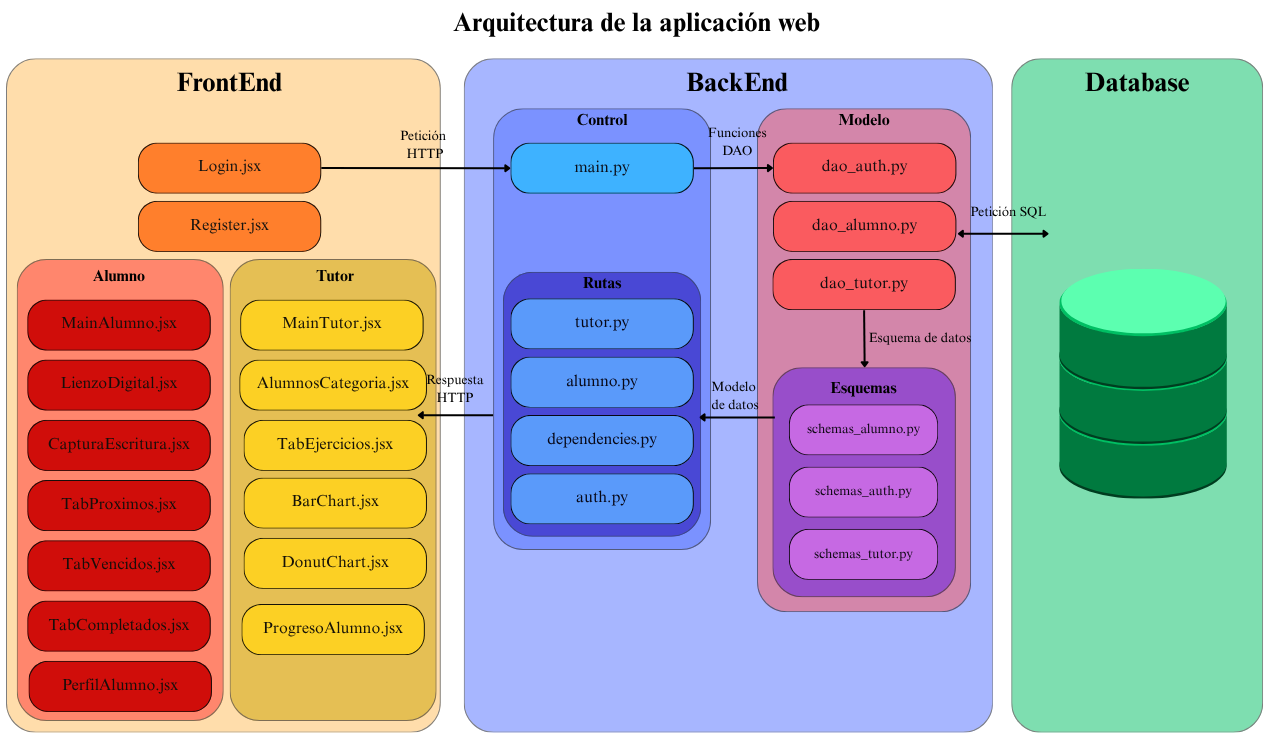
\includegraphics[width=0.95\linewidth]{Imagenes/Arquitectura.png}
        \caption{Diagrama de arquitectura del sistema}
        \label{fig:arquitectura_completa}
    \end{figure}
\end{landscape}

\subsection{Diseño de la base de datos}

El diseño de la base de datos define la capa de persistencia necesaria para soportar las operaciones de la plataforma, garantizando la integridad, seguridad y disponibilidad de la información. Siguiendo las formas normales para el modelado de bases de datos relacionalesw, el esquema ha sido normalizado hasta la Tercera Forma Normal (3NF), lo que permite mitigar anomalías de inserción, actualización y borrado, asegurando que la información de los usuarios y los resultados del análisis se almacenen de manera eficiente y sin redundancias innecesarias. 

En este apartado se detalla el modelo estructurado para gestionar la interacción entre los actores del sistema (tutores y alumnos), el almacenamiento del catálogo de ejercicios y la trazabilidad de la actividad académica. Asimismo, se describe la estrategia de almacenamiento empleada para registrar de forma eficiente las cargas útiles de imágenes y los resultados derivados del procesamiento asíncrono de los módulos de Inteligencia Artificial (OCR y NLP), fundamentando así la generación de recomendaciones personalizadas dentro de la arquitectura del sistema.

\subsubsection{Diagrama entidad-relación}
El diagrama entidad–relación constituye un elemento fundamental dentro del diseño de la aplicación web, ya que permite estructurar de manera formal la organización, almacenamiento y relación de los datos involucrados en el proceso de captura, procesamiento y evaluación de la escritura manuscrita.

La aplicación web propuesta gestiona el proceso de aprendizaje y evaluación de la escritura en alumnos de educación primaria. En este contexto, un tutor es responsable de supervisar a múltiples alumnos, asignándoles ejercicios orientados al desarrollo de habilidades de escritura.

El núcleo del sistema se encuentra en la entidad Intento, la cual representa cada ejecución de un ejercicio por parte del alumno. A partir de este intento, se procesa una imagen mediante OCR para obtener el texto digital, el cual es posteriormente analizado mediante NLP para evaluar la ortografía. De forma complementaria, se realiza un análisis caligráfico basado en características del trazo manuscrito.

Los resultados de estos análisis permiten generar recomendaciones personalizadas y actualizar el progreso del alumno, facilitando el seguimiento continuo de su desempeño.

En la Figura \ref{fig:er} se presenta el diagrama entidad–relación, el cual describe la estructura de datos y las relaciones entre las entidades involucradas en el proceso de evaluación de la escritura.

\begin{landscape}
\centering

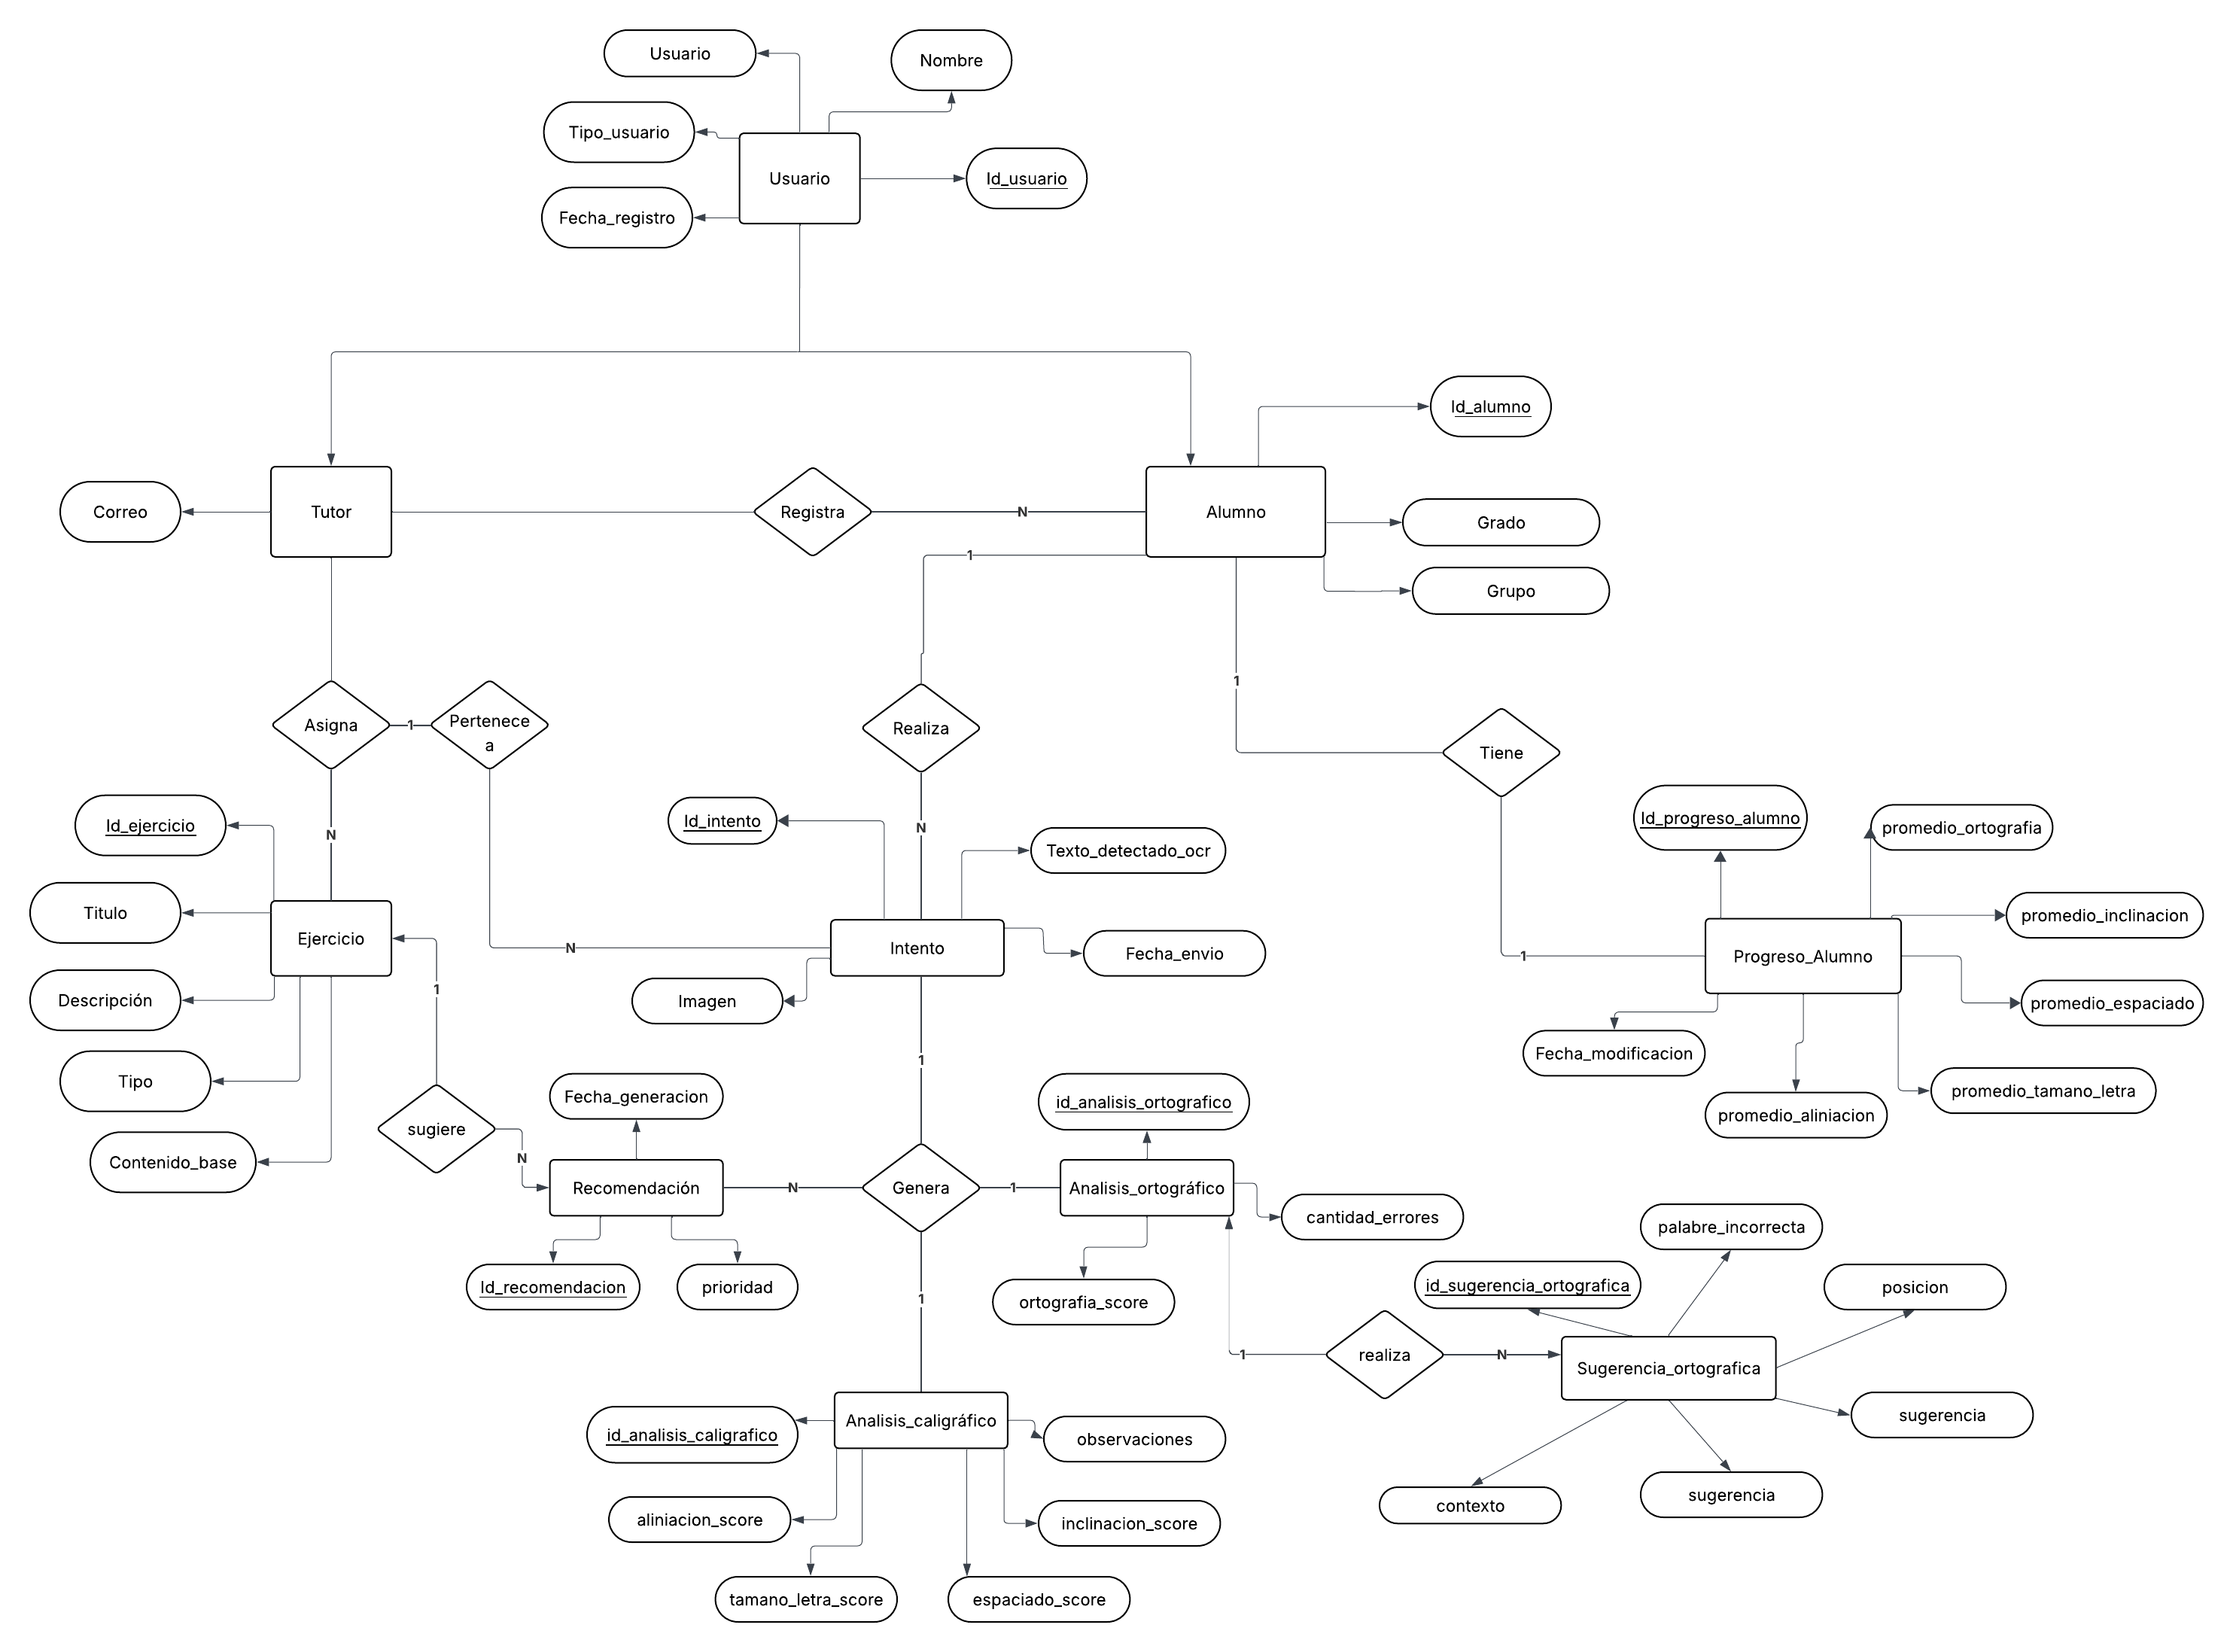
\includegraphics[
    width=0.95\linewidth,
    height=0.95\textheight,
    keepaspectratio
]{Imagenes/Diagrama-entidad-relacion.png}

\captionof{figure}{Diagrama entidad--relación propuesto}
\label{fig:er}

\end{landscape}

\subsubsection{Diccionario de entidades}

\textbf{A. Gestión de usuarios}

En la Tabla \ref{tab:entidades_usuarios} se describen las entidades correspondientes a la gestión de usuarios.

\begin{longtable}{|p{3.5cm}|p{7cm}|p{5cm}|}
\caption{Entidades de gestión de usuarios.}
\label{tab:entidades_usuarios} \\ \hline

\textbf{Entidad} & \textbf{Descripción} & \textbf{Atributos clave} \\ \hline
\endfirsthead

\hline
\textbf{Entidad} & \textbf{Descripción} & \textbf{Atributos clave} \\ \hline
\endhead

Estatus & Entidad que permite indicar el estado de un registro, facilitando su control sin eliminación física. &
id\_estatus, descripcion \\ \hline

Usuario & Entidad base para el acceso a la aplicación web. &
id\_usuario, nombre, tipo\_usuario, fecha\_registro, FK id\_estatus \\ \hline

Tutor & Usuario con permisos para registrar alumnos y asignar ejercicios. &
correo \\ \hline

Alumno & Usuario final que realiza los ejercicios de escritura. &
id\_alumno, grado, grupo \\ \hline

\end{longtable}

Las entidades presentadas permiten gestionar el acceso y la organización de los usuarios dentro del sistema.

\textbf{B. Proceso de evaluación}

En la Tabla \ref{tab:entidades_evaluacion} se presentan las entidades relacionadas con el proceso de evaluación de la escritura.

\begin{longtable}{|p{3.5cm}|p{7cm}|p{5cm}|}
\caption{Entidades del proceso de evaluación del sistema}
\label{tab:entidades_evaluacion} \\ \hline

\textbf{Entidad} & \textbf{Descripción} & \textbf{Atributos clave} \\ \hline
\endfirsthead

\hline
\textbf{Entidad} & \textbf{Descripción} & \textbf{Atributos clave} \\ \hline
\endhead

Ejercicio & Catalogo de ejercicios. &
id\_ejercicio, titulo, contenido\_base, tipo \\ \hline

Ejercicio\_Tutor & Ejercicios asignados por el tutor. & id\_ejercicio\_tutor, FK id\_tutor, FK id\_ejercicio, fecha\_inicio y fecha\_fin, FK id\_estatus\\ \hline

Intento & Ejecución de un ejercicio por parte del alumno. &
id\_intento, FK id\_alumno, FK id\_ejercicio\_tutor, imagen, texto\_detectado\_ocr, fecha\_envio \\ \hline

Analisis\_ortografico & Resultado del procesamiento NLP. &
id\_analisis\_ortografico, cantidad\_errores, ortografia\_score \\ \hline

sugerencia\_ortogra-
fica & Errores detetctados del procesamiento NLP, en conjunto con su sugerencia. &
id\_sugerencia\_ortografica, palabra\_incorrecta, posicion, sugerencia, contexto \\ \hline

Analisis\_caligrafico & Resultado del análisis del trazo manuscrito. &
id\_analisis\_caligrafico, inclinacion\_score, espaciado\_score, tamano\_letra\_score \\ \hline

\end{longtable}

Estas entidades representan el núcleo del procesamiento de la información dentro de la aplicación web.

\textbf{C. Seguimiento y retroalimentación}

En la Tabla \ref{tab:entidades_SR} se describen las entidades asociadas al seguimiento y retroalimentación del alumno.

\begin{longtable}{|p{3.5cm}|p{7cm}|p{5cm}|}
\caption{Entidades del proceso de evaluación del sistema}
\label{tab:entidades_SR} \\ \hline

\textbf{Entidad} & \textbf{Descripción} & \textbf{Atributos clave} \\ \hline
\endfirsthead

\hline
\textbf{Entidad} & \textbf{Descripción} & \textbf{Atributos clave} \\ \hline
\endhead

Recomendación & Sugerencia generada automáticamente. &
id\_recomendacion, FK Id\_intento, FK id\_ejercicio, fecha\_generación, estado, prioridad. \\ \hline

Progreso\_alumno & Indicadores acumulados del desempeño. &
id\_progreso\_alumno,FK id\_alumno,promedio\_orto-
grafia, promedio\_caligrafia \\ \hline

\end{longtable}

Estas entidades permiten el seguimiento del desempeño y la generación de retroalimentación personalizada.



\subsubsection{Análisis de relaciones}

El modelo entidad--relación define las interacciones entre las entidades del sistema mediante relaciones con cardinalidades específicas, las cuales permiten representar la forma en que los datos se asocian dentro del proceso de evaluación de la escritura.

A continuación, se describen las principales relaciones identificadas en el modelo:

\begin{itemize}
    \item \textbf{Herencia (Usuario $\rightarrow$ Tutor / Alumno)}
\end{itemize}

Se establece una relación de especialización en la cual la entidad Usuario actúa como entidad base, de la que derivan los roles de Tutor y Alumno. Esta estructura permite reutilizar atributos comunes, como nombre y fecha de registro, y asignar funcionalidades específicas según el tipo de usuario.

\begin{itemize}
    \item \textbf{Tutor -- Alumno (1:N)}
\end{itemize}

Un tutor puede supervisar a muchos alumnos, mientras que cada alumno está asociado a un único tutor responsable.

\begin{itemize}
    \item \textbf{Tutor -- Ejercicio (M:N)}
\end{itemize}

Un tutor puede asignar múltiples ejercicios del catálogo, y un mismo 
ejercicio del catálogo puede ser asignado por múltiples tutores. Esta 
relación se en la entidad de asociación \textit{Ejercicio\_Tutor}.

\begin{itemize}
    \item \textbf{Alumno -- Intento (1:N)}
\end{itemize}

Un alumno puede realizar múltiples intentos a lo largo del tiempo, ya que cada intento representa una ejecución individual de un ejercicio. Esta relación permite almacenar el historial de participación del alumno.

\begin{itemize}
    \item \textbf{Intento -- Análisis ortográfico (1:1)}
\end{itemize}

Cada intento genera exactamente un análisis ortográfico, el cual contiene la evaluación del texto detectado mediante NLP, incluyendo errores y sugerencias.

\begin{itemize}
    \item \textbf{Intento -- Análisis caligráfico (1:1)}
\end{itemize}

Cada intento genera un único análisis caligráfico, el cual evalúa características del trazo manuscrito como alineación, tamaño y espaciado.

\begin{itemize}
    \item \textbf{Intento -- Recomendación (1:N)}
\end{itemize}

Un intento puede generar múltiples recomendaciones, dependiendo de la cantidad y tipo de errores detectados en los análisis realizados.

\begin{itemize}
    \item \textbf{Alumno -- Progreso\_alumno (1:1)}
\end{itemize}

Cada alumno cuenta con un único registro en la entidad Progreso\_alumno, el cual almacena indicadores acumulados de su desempeño, como promedios de ortografía y caligrafía.

Esta relación nos permite obtener un promedio global para el análisis ortográfico y caligráfico, facilitando la calsificación de los alumnos.

\subsubsection{Diagrama relacional}

En la Figura \ref{fig:rel} se presenta el diagrama relacional de la aplicación web, donde se definen las tablas, sus atributos, así como las relaciones mediante llaves primarias y foráneas.

\begin{landscape}
    
\begin{figure}[H]
    \centering
    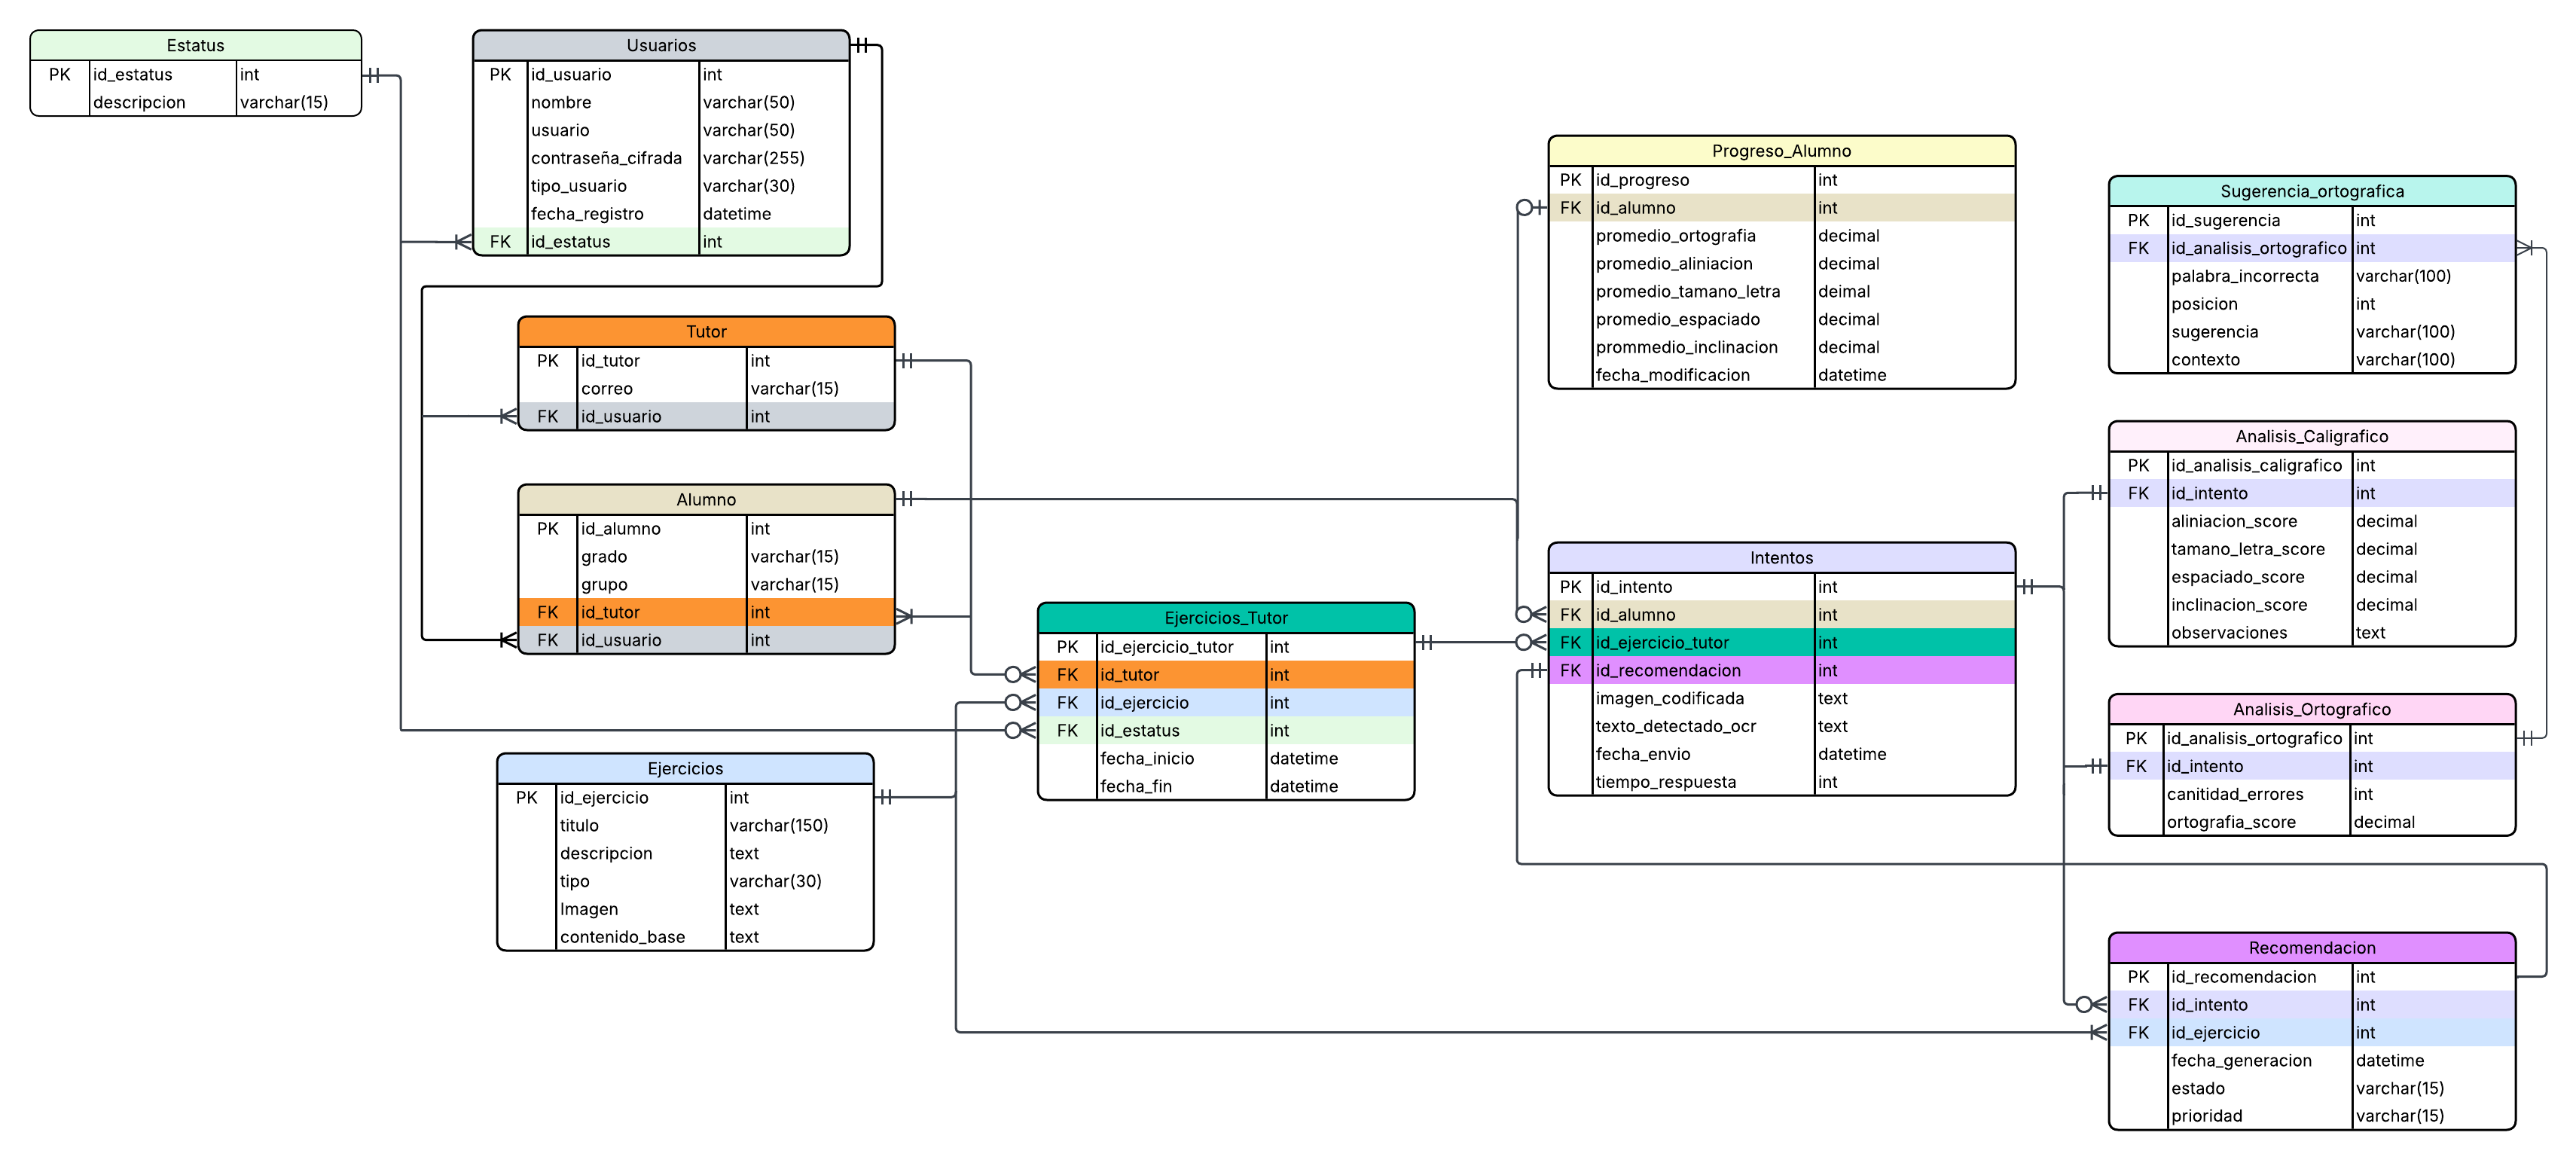
\includegraphics[
        width=\linewidth,
        keepaspectratio
    ]{Imagenes/DiagramaRelaiconal-2.png}

    \caption{Diagrama relacional propuesto}
    \label{fig:rel}
\end{figure}

\end{landscape}

\subsubsection{Decisiones de diseño de base de datos}

\paragraph{Gestión del texto detectado (OCR)}

El atributo texto\_detectado\_ocr en la entidad Intento representa un elemento crítico dentro de la aplicación web, ya que corresponde a la salida generada por el módulo de reconocimiento óptico de caracteres (OCR). Este dato constituye la entrada principal para el procesamiento mediante técnicas de procesamiento de lenguaje natural (NLP), por lo que su correcta generación y almacenamiento es fundamental para garantizar la calidad del análisis ortográfico.

El uso de este formato proporciona flexibilidad y evita la rigidez de un esquema relacional estrictamente normalizado, facilitando futuras ampliaciones del sistema.

\paragraph{Cálculo del progreso del alumno}

La entidad \textit{Progreso\_alumno} funciona como una tabla de agregación que almacena indicadores globales del desempeño del estudiante. Su actualización se realiza mediante triggers a nivel de base de datos, los cuales recalculan automáticamente los promedios de ortografía y caligrafía al registrar un nuevo inteno.

Este enfoque se justifica por las siguientes razones:

\begin{itemize}
    \item \textbf{Atomicidad:} el trigger se ejecuta dentro de la misma transacción que el INSERT del intento, garantizando que \textit{Progreso\_alumno} siempre refleje el estado actualizado sin depender de una llamada adicional desde el controlador.

    \item \textbf{Consistencia:} se elimina el riesgo de inconsistencia de datos ante un fallo del backend posterior a la inserción del intento pero previo a la actualización del progreso.

    \item \textbf{Separación de responsabilidades:} el controlador no requiere conocer la lógica de cálculo de promedios, delegando esa responsabilidad a la base de datos, lo cual es coherente con el patrón de diseño MVC adoptado en el sistema.

\end{itemize}

\paragraph{Gestión del historial y trazabilidad}

La vista \textit{vw\_historial\_alumno} permite mantener un registro cronológico de los resultados obtenidos por el alumno en cada intento, sin comprometer la normalización del modelo de datos. A diferencia de una tabla adicional, la vista consolida la información existente en las entidades Intento, Analisis\_ortografico y Analisis\_caligrafico mediante una consulta predefinida, evitando la redundancia de datos. 

\subsection{Diagrama de clases del sistema}

Con el objetivo de definir la estructura estática del sistema, se presenta el diagrama de clases, el cual describe las principales entidades, sus atributos y las relaciones existentes entre ellas.

\begin{figure}[H]
    \centering
    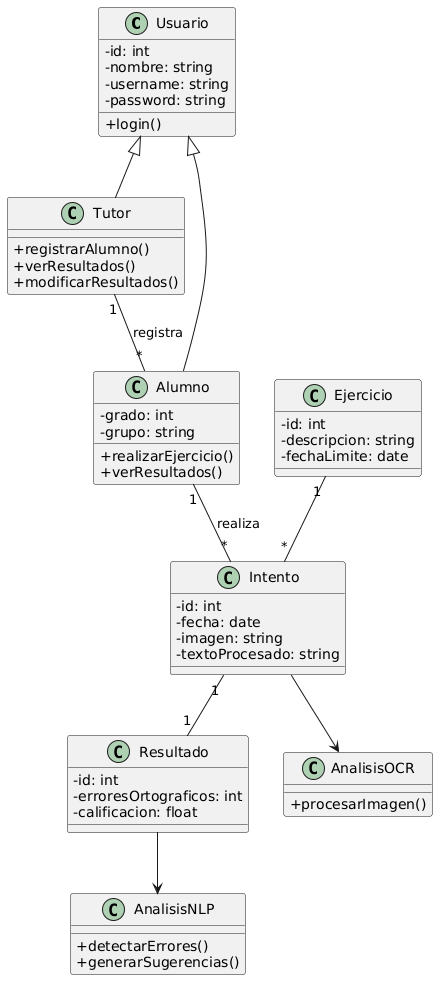
\includegraphics[width=0.60\textwidth]{Imagenes/DiagramaDeClases.png}
    \caption{Diagrama de clases del sistema}
    \label{fig:diagrama_clases}
\end{figure}

El diagrama de clases representa la estructura estática del sistema, mostrando las principales entidades, sus atributos y las relaciones entre ellas. Se observa una jerarquía de herencia donde la clase \textit{Usuario} es la base para los actores \textit{Tutor} y \textit{Alumno}. Asimismo, se modelan los elementos centrales del sistema como \textit{Ejercicio}, \textit{Intento} y \textit{Resultado}, los cuales permiten gestionar el proceso de captura, análisis y retroalimentación de la escritura. Finalmente, se integran los módulos de procesamiento \textit{AnalisisOCR} y \textit{AnalisisNLP}, responsables de la conversión de imágenes a texto y la detección de errores ortográficos respectivamente.

%------------------------------------------------

\subsection{Diagrama de secuencia del procesamiento de ejercicios}

Con el propósito de representar el comportamiento dinámico del sistema, se presenta el diagrama de secuencia correspondiente al proceso de análisis de ejercicios, el cual describe la interacción entre los diferentes componentes involucrados desde la captura de la imagen hasta la generación de resultados.

\begin{figure}[H]
    \centering
    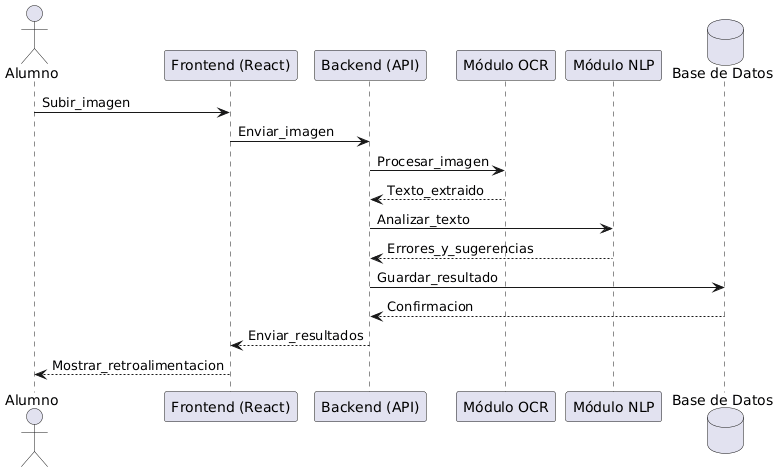
\includegraphics[width=0.75\textwidth]{Imagenes/DiagramaDeSecuencia.png}
    \caption{Diagrama de secuencia del procesamiento de ejercicios}
    \label{fig:diagrama_secuencia}
\end{figure}

El diagrama muestra cómo el alumno interactúa con la interfaz para enviar una imagen, la cual es procesada por el backend mediante un módulo OCR para la extracción de texto. Posteriormente, el texto es analizado por el módulo NLP para identificar errores ortográficos y generar sugerencias. Finalmente, los resultados son almacenados en la base de datos y enviados al usuario para su visualización.

%------------------------------------------------

\subsection{Diagrama de actividad del procesamiento de ejercicios}

Con el propósito de representar el flujo de actividades del sistema, se presenta el diagrama de actividad correspondiente al proceso de análisis de ejercicios, el cual describe de manera secuencial las acciones realizadas desde la interacción del usuario hasta la generación de resultados.

\begin{figure}[H]
    \centering
    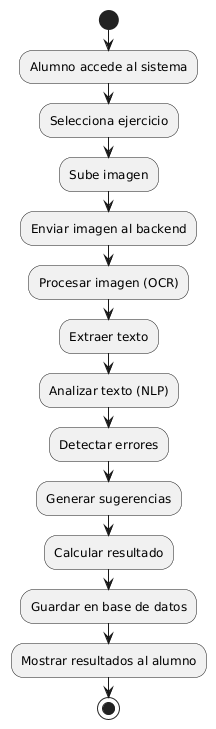
\includegraphics[width=0.35\textwidth]{Imagenes/DiagramaDeActividad.png}
    \caption{Diagrama de actividad del procesamiento de ejercicios}
    \label{fig:diagrama_actividad}
\end{figure}

El diagrama muestra la secuencia de actividades que se llevan a cabo cuando un alumno realiza un ejercicio, comenzando desde la selección y envío de la imagen, pasando por el procesamiento mediante OCR y el análisis con técnicas de procesamiento de lenguaje natural, hasta la generación y almacenamiento de los resultados, los cuales son finalmente presentados al usuario.

%------------------------------------------------

%\subsection{Diagrama de estados del proceso de evaluación}

%Con el propósito de representar los diferentes estados por los que pasa un ejercicio dentro del sistema, se presenta el diagrama de estados, el cual describe el ciclo de vida del proceso de evaluación desde su inicio hasta la presentación de resultados.

%\begin{figure}[H]
%    \centering
%    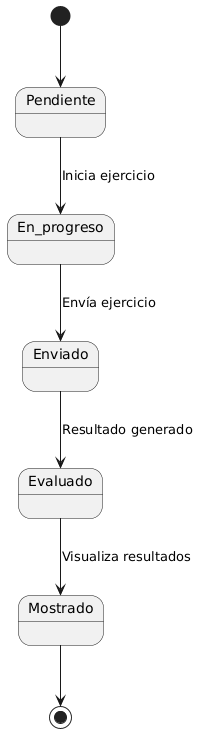
\includegraphics[width=0.60\textwidth]{Imagenes/DiagramaDeEstado.png}
%    \caption{Diagrama de estados del proceso de evaluación}
%    \label{fig:diagrama_estados}
%\end{figure}

%El diagrama muestra los estados principales por los que transita un ejercicio dentro del sistema, desde que se encuentra pendiente, pasando por su desarrollo y envío, hasta su evaluación y visualización por parte del usuario. Este modelo permite comprender el comportamiento general del sistema durante el proceso de evaluación sin detallar los procesos internos.
            
%------------------------------------------------

\subsection{Diagrama de componentes del sistema}

Con el objetivo de representar la estructura modular del sistema, se presenta el diagrama de componentes, el cual muestra la organización de los principales elementos de software y sus interacciones dentro de la arquitectura de la aplicación.

\begin{figure}[H]
    \centering
    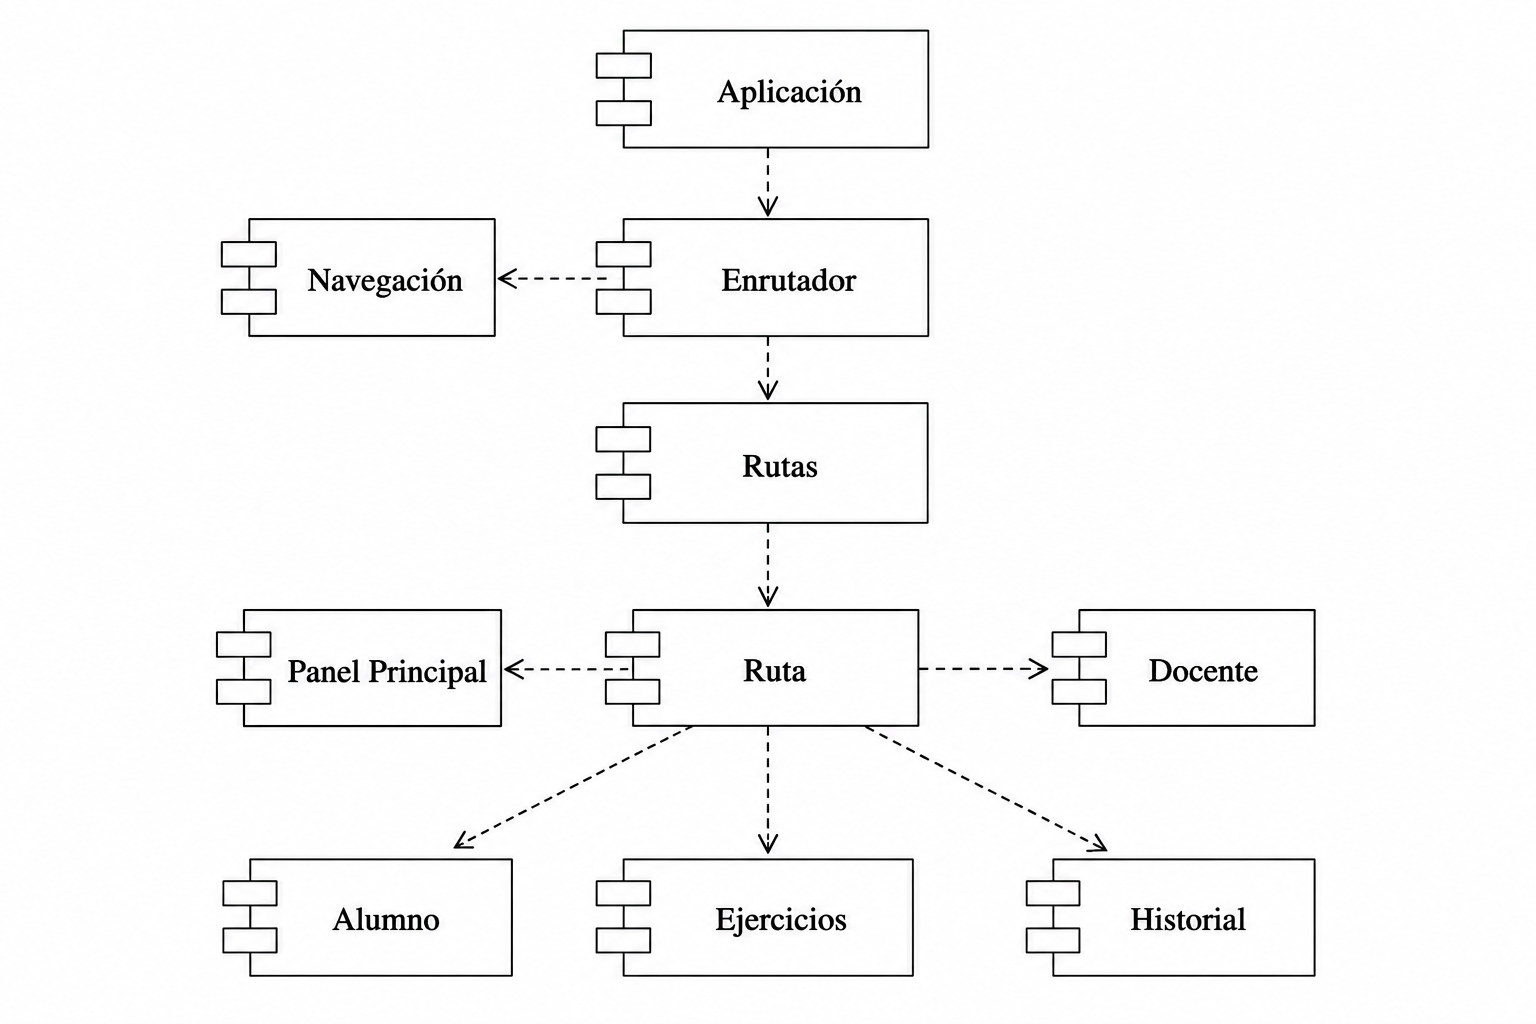
\includegraphics[width=0.65\textwidth]{Imagenes/DiagramaDeComponentess.png}
    \caption{Diagrama de componentes del sistema}
    \label{fig:diagrama_componentes}
\end{figure}

El diagrama muestra la separación del sistema en tres capas principales: cliente, servidor y persistencia. El frontend se encarga de la interacción con el usuario, mientras que el backend gestiona la lógica del sistema y coordina el procesamiento mediante los módulos OCR y NLP. Finalmente, la base de datos permite almacenar la información generada y consultada durante la operación del sistema.

La separación de los módulos de procesamiento OCR y NLP permite una arquitectura más flexible y escalable, ya que cada componente puede ser optimizado o actualizado de manera independiente. Además, esta división facilita el mantenimiento del sistema y mejora la eficiencia en el procesamiento de la información.

%------------------------------------------------

\subsection{Diagrama de despliegue del sistema}

Con el objetivo de representar la distribución física del sistema, se presenta el diagrama de despliegue, el cual muestra los nodos de hardware involucrados y la forma en que los componentes de software se encuentran distribuidos dentro de la arquitectura de la aplicación.

\begin{figure}[H]
    \centering
    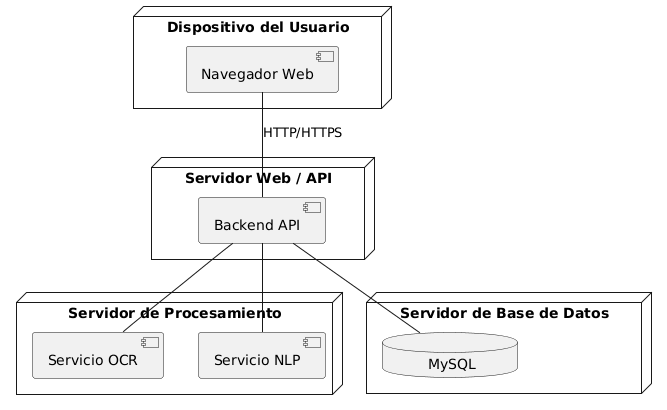
\includegraphics[width=0.65\textwidth]{Imagenes/DiagramaDeDespliegue.png}
    \caption{Diagrama de despliegue del sistema}
    \label{fig:diagrama_despliegue}
\end{figure}

El diagrama muestra la organización del sistema en distintos nodos físicos, incluyendo el dispositivo del usuario, el servidor de aplicaciones, el servidor de procesamiento y el servidor de base de datos. En el dispositivo del usuario se ejecuta el navegador web, desde donde se realizan las solicitudes al backend mediante protocolos HTTP/HTTPS. El servidor de aplicaciones gestiona la lógica del sistema, mientras que los servicios de procesamiento OCR y NLP se encargan de analizar la información recibida. Finalmente, el servidor de base de datos permite almacenar y consultar la información generada durante la operación del sistema.

Asimismo, se observa la separación de los servicios en distintos nodos, lo cual permite una mejor distribución de la carga y facilita la escalabilidad del sistema.
%% ─────────────────────────────────────────────────────────────────────────────
%  Sección 4.X  Arquitectura del Módulo de Gestión de Ejercicios
%  Insertar en el Capítulo 4: Diseño, después del módulo de Autenticación
%  y antes del módulo OCR/NLP.
% ─────────────────────────────────────────────────────────────────────────────

\subsection{Arquitectura del Módulo de Gestión de Ejercicios}

El módulo de gestión de ejercicios administra el ciclo de vida completo
de las actividades de escritura dentro de la plataforma. Su diseño contempla
dos actores con responsabilidades distintas: el tutor, que selecciona
ejercicios del catálogo y los asigna a sus alumnos con una vigencia
determinada; y el alumno, que consulta los ejercicios disponibles
clasificados por su estado. El módulo también incorpora un proceso
automatizado que cierra los ejercicios cuya fecha de vencimiento ha
sido alcanzada, garantizando la coherencia del estado del sistema sin
intervención manual.

La arquitectura del módulo se divide en tres componentes principales:

\begin{enumerate}
    \item \textbf{Capa de Presentación (Front-End):} Compuesta por los
    componentes \texttt{TabEjercicios.jsx} (vista del tutor para gestionar
    asignaciones), \texttt{TabProximos.jsx}, \texttt{TabCompletados.jsx}
    y \texttt{TabVencidos.jsx} (vistas del alumno que clasifican los
    ejercicios según su estado). Cada componente consulta su endpoint
    correspondiente y renderiza la información sin lógica de negocio
    propia.

    \item \textbf{Capa de Lógica de Negocio (Back-End):} Implementada
    en el controlador \texttt{ejercicios.py} mediante FastAPI. Gestiona
    la consulta del catálogo, la activación y desactivación de ejercicios
    por parte del tutor, y la consulta de ejercicios en sus tres estados
    posibles desde la perspectiva del alumno. Adicionalmente, el proceso
    \texttt{cerrar\_ejercicio.py} implementa un scheduler que verifica
    y cierra automáticamente los ejercicios vencidos cada hora.

    \item \textbf{Capa de Persistencia (Base de Datos):} El módulo opera
    sobre dos tablas principales: \texttt{Ejercicios}, que actúa como
    catálogo inmutable de actividades disponibles en la plataforma, y
    \texttt{Ejercicios\_Tutor}, que representa la asignación de un
    ejercicio del catálogo a un tutor específico, con su propio ciclo de
    vida controlado por el campo \texttt{id\_estatus} y la fecha
    \texttt{fecha\_desactivacion}.
\end{enumerate}

% ─────────────────────────────────────────────────────────
\subsubsection{Diseño del Ciclo de Vida de un Ejercicio}

Un ejercicio atraviesa los siguientes estados a lo largo de su ciclo de
vida dentro del sistema:

\begin{enumerate}
    \item \textbf{Disponible en catálogo:} el ejercicio existe en la tabla
    \texttt{Ejercicios} con \texttt{id\_estatus = 1} y puede ser
    seleccionado por cualquier tutor para su asignación.

    \item \textbf{Activo:} el tutor ha creado un registro en
    \texttt{Ejercicios\_Tutor} con \texttt{id\_estatus = 1}. A partir de
    este momento, el ejercicio es visible para los alumnos del tutor en
    su panel de ejercicios próximos.

    \item \textbf{Vencido:} el ejercicio transiciona a
    \texttt{id\_estatus = 2} por uno de dos mecanismos: desactivación
    manual por parte del tutor mediante el endpoint de eliminación, o
    cierre automático por el scheduler cuando la fecha
    \texttt{fecha\_desactivacion} es anterior a la fecha y hora actuales
    del servidor. Un ejercicio vencido deja de aparecer en la lista de
    próximos del alumno y pasa a la lista de vencidos si no fue entregado,
    o permanece en completados si el alumno ya realizó un intento.
\end{enumerate}

\noindent \textit{Nota de diseño}: el sistema no elimina físicamente los
registros de \texttt{Ejercicios\_Tutor}. La transición entre estados se
gestiona exclusivamente mediante el campo \texttt{id\_estatus}, lo que
preserva la trazabilidad histórica de las asignaciones y permite al tutor
consultar ejercicios previamente activos sin pérdida de información.

% ─────────────────────────────────────────────────────────
\subsubsection{Diseño del Flujo de Interacción}

El módulo contempla tres flujos principales de interacción.

\textbf{Flujo de Asignación de Ejercicio (Tutor):}
\begin{enumerate}
    \item El tutor accede a su panel y solicita el catálogo de ejercicios
    disponibles mediante una petición \texttt{GET} al endpoint público
    \texttt{/api/ejercicios/}.
    \item El tutor selecciona un ejercicio y establece opcionalmente una
    fecha de vencimiento. El Front-End envía una petición \texttt{POST}
    al endpoint \texttt{/api/ejercicios/tutor} con el identificador del
    ejercicio y la fecha de cierre.
    \item El Back-End verifica mediante JWT que el \texttt{id\_usuario}
    del token coincide con el \texttt{id\_usuario} del payload, evitando
    que un tutor active ejercicios en nombre de otro.
    \item Se verifica que el tutor no tenga ya activo el mismo ejercicio.
    En caso de duplicado, se retorna \texttt{400 Bad Request}.
    \item Se inserta un nuevo registro en \texttt{Ejercicios\_Tutor} con
    \texttt{id\_estatus = 1}. El ejercicio queda inmediatamente disponible
    para los alumnos del tutor.
\end{enumerate}

\textbf{Flujo de Consulta de Ejercicios (Alumno):}

Desde la perspectiva del alumno, los ejercicios se presentan clasificados
en tres pestañas. La lógica de clasificación reside íntegramente en el
Back-End mediante tres consultas SQL independientes:

\begin{itemize}
    \item \textbf{Próximos:} ejercicios activos (\texttt{id\_estatus = 1})
    asignados por el tutor del alumno que aún no tienen un intento
    registrado por ese alumno. Se excluyen mediante una subconsulta
    \texttt{NOT IN} sobre la tabla \texttt{Intentos}.

    \item \textbf{Completados:} ejercicios que tienen al menos un intento
    registrado por el alumno. Se retorna únicamente el intento más reciente
    por ejercicio, determinado mediante la función de ventana
    \texttt{ROW\_NUMBER() OVER (PARTITION BY id\_ejercicio\_tutor ORDER BY
    fecha\_envio DESC)}, incluyendo la calificación y retroalimentación
    del tutor si ya fueron registradas.

    \item \textbf{Vencidos:} ejercicios con \texttt{id\_estatus = 2} que
    no tienen ningún intento registrado por el alumno, es decir, los que
    el alumno no alcanzó a entregar antes del cierre.
\end{itemize}

\paragraph{Flujo de Cierre Automático (Scheduler):}
\begin{enumerate}
    \item Al iniciar el servidor, el evento \texttt{startup} de FastAPI
    invoca \texttt{iniciar\_scheduler()}, que registra una tarea periódica
    con una frecuencia de ejecución de una hora mediante la biblioteca
    APScheduler.
    \item Cada hora, la tarea \texttt{cerrar\_ejercicios\_vencidos()}
    ejecuta un \texttt{UPDATE} sobre la tabla \texttt{Ejercicios\_Tutor},
    transitando a \texttt{id\_estatus = 2} todos los registros cuya
    \texttt{fecha\_desactivacion} sea distinta de nulo y anterior a la
    fecha y hora actuales del servidor (\texttt{GETDATE()}).
    \item La operación es idempotente: ejecutarla múltiples veces sobre
    los mismos datos no produce efectos secundarios, ya que la condición
    \texttt{id\_estatus = 1} del filtro impide modificar registros ya
    cerrados.
\end{enumerate}

% ─────────────────────────────────────────────────────────
\subsubsection{Diseño de APIs}

Para soportar los flujos descritos, el diseño de la API contempla los
siguientes endpoints en el controlador \texttt{ejercicios.py}:

\textbf{Endpoint 1:} Consulta del Catálogo

El endpoint \texttt{/api/ejercicios/} opera mediante el método \texttt{GET}
y no requiere autenticación. Retorna todos los ejercicios con
\texttt{id\_estatus = 1} disponibles en la tabla \texttt{Ejercicios}.

\textbf{Endpoint 2:} Consulta de Ejercicios Activos del Tutor

El endpoint \texttt{/api/ejercicios/tutor/\{id\_usuario\}} opera mediante
el método \texttt{GET} y requiere autenticación JWT con rol de tutor.
Retorna los ejercicios que el tutor ha activado y que se encuentran
actualmente con \texttt{id\_estatus = 1}.

\textbf{Endpoint 3:} Activación de Ejercicio

El endpoint \texttt{/api/ejercicios/tutor} opera mediante el método
\texttt{POST} y requiere autenticación JWT con rol de tutor. Recibe el
identificador del ejercicio del catálogo y una fecha de vencimiento
opcional.

\begin{lstlisting}[language=json, caption={Payload de solicitud del endpoint de activación de ejercicio}, label={lst:ejercicio-create}]
/* Solicitud */
{
  "id_ejercicio": <integer>,
  "id_usuario":   <integer>,
  "fecha_fin":    "datetime | null"
}

/* Respuesta 201 Created */
{
  "message": "Ejercicio activado correctamente"
}
\end{lstlisting}

\textbf{Endpoint 4:} Desactivación Manual de Ejercicio

El endpoint \texttt{/api/ejercicios/tutor/\{id\_usuario\}/\{id\_ejercicio\}}
opera mediante el método \texttt{DELETE} y requiere autenticación JWT con
rol de tutor. Actualiza el campo \texttt{id\_estatus} a 2 en el registro
correspondiente de \texttt{Ejercicios\_Tutor}, sin eliminar el registro
físicamente.

\textbf{Endpoints 5, 6 y 7:} Consulta de Ejercicios del Alumno

Los endpoints \texttt{/api/ejercicios/alumno/\{id\_alumno\}/proximos},
\texttt{/api/ejercicios/alumno/\{id\_alumno\}/completados} y
\texttt{/api/ejercicios/alumno/\{id\_alumno\}/vencidos} operan mediante
el método \texttt{GET} y requieren autenticación JWT con rol de alumno.
En los tres casos, el Back-End verifica que el \texttt{id\_alumno} de la
ruta coincida con el \texttt{id\_usuario} del token, retornando
\texttt{403 Forbidden} en caso de discrepancia.

La Tabla~\ref{tab:endpoints-ejercicios} resume los endpoints del módulo
con su método y nivel de acceso correspondiente.

\begin{table}[H]
\centering
\caption{Endpoints del módulo de gestión de ejercicios}
\label{tab:endpoints-ejercicios}
\begin{tabular}{|l|l|l|}
\hline
\textbf{Endpoint} & \textbf{Método} & \textbf{Acceso requerido} \\
\hline
\texttt{/api/ejercicios/}
    & GET    & Público \\
\texttt{/api/ejercicios/tutor/\{id\_usuario\}}
    & GET    & Tutor (JWT) \\
\texttt{/api/ejercicios/tutor}
    & POST   & Tutor (JWT) \\
\texttt{/api/ejercicios/tutor/\{id\_usuario\}/\{id\_ejercicio\}}
    & DELETE & Tutor (JWT) \\
\texttt{/api/ejercicios/alumno/\{id\_alumno\}/proximos}
    & GET    & Alumno (JWT) \\
\texttt{/api/ejercicios/alumno/\{id\_alumno\}/completados}
    & GET    & Alumno (JWT) \\
\texttt{/api/ejercicios/alumno/\{id\_alumno\}/vencidos}
    & GET    & Alumno (JWT) \\
\hline
\end{tabular}
\end{table}

\subsection{Arquitectura del Módulo de Progreso y Recomendaciones}

El módulo de progreso y recomendaciones centraliza el seguimiento
longitudinal del desempeño del alumno y expone al tutor las herramientas
de supervisión grupal necesarias para tomar decisiones pedagógicas
informadas. A diferencia de los módulos anteriores, cuyo alcance es
transaccional —un intento, un ejercicio, una autenticación—, este módulo
opera sobre el historial acumulado del alumno, sintetizando múltiples
análisis en indicadores agregados que reflejan su evolución en el tiempo.

La arquitectura del módulo se divide en tres componentes principales:

\begin{enumerate}
    \item \textbf{Capa de Presentación (Front-End):} Compuesta por el
    componente \texttt{ProgresoAlumnos.jsx} en el panel del tutor, que
    presenta gráficas de dona y de barras con la distribución del grupo
    por categoría de desempeño, y por el componente
    \texttt{PerfilAlumno.jsx} en el panel del alumno, que expone sus
    datos personales y permite actualizarlos. La clasificación del grupo
    se presenta en dos dimensiones independientes —ortografía y
    legibilidad— seleccionables mediante pestañas, con soporte
    responsivo para pantallas móviles.

    \item \textbf{Capa de Lógica de Negocio (Back-End):} Implementada
    en los controladores \texttt{alumnos.py} y \texttt{perfil.py}
    mediante FastAPI. El primero gestiona el registro, la consulta y la
    baja de alumnos, así como la clasificación del grupo por nivel de
    desempeño y la generación de datos para las gráficas de progreso.
    El segundo gestiona las operaciones de actualización de perfil tanto
    del tutor como del alumno.

    \item \textbf{Capa de Persistencia (Base de Datos):} El módulo opera
    principalmente sobre las tablas \texttt{Progreso\_Alumno} e
    \texttt{Historial\_Alumno}. La primera almacena el promedio acumulado
    vigente del alumno en cada dimensión de evaluación; la segunda
    registra una fotografía histórica del progreso cada vez que dicho
    promedio es actualizado, permitiendo trazar la evolución del alumno
    a lo largo del tiempo. Las tablas \texttt{Recomendacion} y
    \texttt{Actividad\_Sugerida} soportan la generación de actividades
    personalizadas a partir de los errores detectados.
\end{enumerate}

% ─────────────────────────────────────────────────────────
\subsubsection{Diseño del Modelo de Progreso}

El progreso del alumno se representa mediante dos dimensiones
independientes pero complementarias:

\begin{itemize}
    \item \textbf{Promedio ortográfico} (\texttt{promedio\_ortografia}):
    promedio acumulado del campo \texttt{ortografia\_score} de todos los
    análisis ortográficos registrados para el alumno.

    \item \textbf{Promedio de legibilidad} (calculado): promedio aritmético
    de los cuatro scores caligráficos —\texttt{alineacion\_score},
    \texttt{tamano\_letra\_score}, \texttt{espaciado\_score} e
    \texttt{inclinacion\_score}— derivados de los análisis caligráficos
    del alumno.
\end{itemize}

El \textbf{promedio general} se obtiene como la media de ambas
dimensiones y actúa como indicador sintético para la clasificación del
alumno dentro de su grupo:

\begin{equation}
    Promedio\_general = \frac{Promedio\_ortográfico +
    Promedio\_legibilidad}{2}
    \label{eq:promedio-general}
\end{equation}

Con base en el promedio general, el sistema clasifica a cada alumno en
una de tres categorías, conforme a la Tabla~\ref{tab:categorias-progreso}:

\begin{table}[H]
\centering
\caption{Categorías de clasificación de alumnos por promedio general}
\label{tab:categorias-progreso}
\begin{tabular}{|l|l|p{7cm}|}
\hline
\textbf{Categoría} & \textbf{Rango} & \textbf{Interpretación} \\
\hline
En riesgo   & $< 6.0$         & El alumno presenta deficiencias significativas en
                                 ortografía o legibilidad que requieren atención
                                 prioritaria del tutor. \\
Regular     & $[6.0, \ 8.0]$  & El alumno mantiene un desempeño aceptable con
                                 áreas de oportunidad identificadas. \\
Excelencia  & $> 8.0$         & El alumno muestra un desempeño consistentemente
                                 alto en ambas dimensiones evaluadas. \\
\hline
\end{tabular}
\end{table}
\newpage
\noindent\textbf{Nota de diseño:} los umbrales de clasificación (6.0 y
8.0) están alineados con la escala de evaluación del sistema educativo
mexicano de educación primaria \cite{sep2011guia}, donde 6.0 representa
el mínimo aprobatorio y 8.0 delimita el desempeño sobresaliente.

% ─────────────────────────────────────────────────────────
\subsubsection{Diseño del Flujo de Actualización de Progreso}

La tabla \texttt{Progreso\_Alumno} se actualiza cada vez que el módulo
OCR/NLP completa el análisis de un intento. El mecanismo de actualización
opera en dos pasos:

\begin{enumerate}
    \item \textbf{Actualización del promedio vigente:} al persistir los
    resultados de \texttt{Analisis\_Ortografico} y
    \texttt{Analisis\_Caligrafico}, el proceso recalcula los promedios
    acumulados del alumno mediante una consulta \texttt{UPDATE} con
    subconsulta \texttt{AVG} sobre todos sus intentos analizados hasta
    la fecha, y los escribe en \texttt{Progreso\_Alumno}.

    \item \textbf{Registro histórico:} simultáneamente, se inserta un
    nuevo registro en \texttt{Historial\_Alumno} con una instantánea
    (\textit{snapshot}) del progreso en ese momento, incluyendo la fecha
    con precisión \texttt{DATETIME2}. Este registro es inmutable y
    permite reconstruir la curva de progreso del alumno a lo largo del
    tiempo, independientemente de los cambios posteriores en
    \texttt{Progreso\_Alumno}.
\end{enumerate}

La separación entre la tabla de progreso vigente y la tabla de historial
responde a una decisión de diseño deliberada: \texttt{Progreso\_Alumno}
es la fuente de verdad para las consultas actuales del tutor y los
cálculos de clasificación, mientras que \texttt{Historial\_Alumno}
es la fuente de verdad para la visualización de la evolución temporal.
Ambas responsabilidades son distintas y justifican la existencia de dos
tablas separadas.

% ─────────────────────────────────────────────────────────
\subsubsection{Diseño del Flujo de Recomendaciones}

Cuando el análisis de un intento es completado, el sistema genera
recomendaciones de actividades personalizadas para el alumno. El flujo
es el siguiente:

\begin{enumerate}
    \item El proceso evalúa los resultados del análisis recién
    completado e identifica el tipo de error predominante: ortográfico
    si \texttt{ortografia\_score} está por debajo del umbral, caligráfico
    si alguno de los cuatro scores de legibilidad lo está.

    \item Se consulta la tabla \texttt{Actividad\_Sugerida} filtrando por
    \texttt{tipo\_error} y \texttt{tipo\_ejercicio} correspondientes al
    error identificado.

    \item Se insertan registros en la tabla \texttt{Recomendacion}
    vinculando el \texttt{id\_intento} con las actividades seleccionadas.
    Cada recomendación recibe un valor de \texttt{prioridad}
    (\texttt{alta}, \texttt{media} o \texttt{baja}) calculado con base
    en la magnitud del error: a mayor desviación respecto al umbral,
    mayor prioridad.

    \item El alumno consulta sus recomendaciones pendientes, ordenadas
    por prioridad, desde su panel. Al realizar una actividad sugerida,
    el campo \texttt{estado} de la recomendación transiciona de
    \texttt{pendiente} a \texttt{completada}.
\end{enumerate}

% ─────────────────────────────────────────────────────────
\subsubsection{Diseño de APIs}

Para soportar los flujos descritos, el diseño de la API contempla los
siguientes endpoints distribuidos entre los controladores
\texttt{alumnos.py} y \texttt{perfil.py}:

\paragraph{Endpoints de gestión de alumnos (tutor)}

\begin{table}[H]
\centering
\caption{Endpoints de gestión de alumnos}
\label{tab:endpoints-alumnos}
\begin{tabular}{|l|l|l|}
\hline
\textbf{Endpoint} & \textbf{Método} & \textbf{Acceso} \\
\hline
\texttt{/api/alumnos/registrar}              & POST & Tutor (JWT) \\
\texttt{/api/alumnos/tutor/\{id\_tutor\}}    & GET  & Tutor (JWT) \\
\texttt{/api/alumnos/baja/\{id\_alumno\}}    & PUT  & Tutor (JWT) \\
\hline
\end{tabular}
\end{table}

\paragraph{Endpoints de clasificación y progreso grupal (tutor)}

Los siguientes tres endpoints implementan la clasificación del grupo
según las categorías definidas en la Tabla~\ref{tab:categorias-progreso}.
Cada uno ejecuta la misma consulta CTE (\textit{Common Table Expression})
sobre \texttt{Progreso\_Alumno}, variando únicamente el filtro de
\texttt{promedio\_general} aplicado:

\begin{table}[H]
\centering
\caption{Endpoints de clasificación de alumnos por desempeño}
\label{tab:endpoints-clasificacion}
\begin{tabular}{|l|l|l|}
\hline
\textbf{Endpoint} & \textbf{Método} & \textbf{Acceso} \\
\hline
\texttt{/api/alumnos/riesgo/\{id\_tutor\}}      & GET & Tutor (JWT) \\
\texttt{/api/alumnos/regular/\{id\_tutor\}}     & GET & Tutor (JWT) \\
\texttt{/api/alumnos/excelencia/\{id\_tutor\}}  & GET & Tutor (JWT) \\
\hline
\end{tabular}
\end{table}

El endpoint \texttt{/api/alumnos/progreso/\{id\_tutor\}} opera mediante
el método \texttt{GET} y retorna los datos agrupados para las gráficas
del panel del tutor. Ejecuta dos consultas independientes: una sobre
el promedio ortográfico y otra sobre el promedio de legibilidad,
retornando para cada dimensión la cantidad de alumnos por categoría.

\begin{lstlisting}[language=json, caption={Estructura de respuesta del endpoint de progreso gráfico}, label={lst:progreso-response}]
/* Respuesta 200 OK */
{
  "ortografia": [
    { "categoria": "Buen Promedio",    "cantidad_alumnos": <int> },
    { "categoria": "Promedio Regular", "cantidad_alumnos": <int> },
    { "categoria": "Mal Promedio",     "cantidad_alumnos": <int> }
  ],
  "legibilidad": [
    { "categoria": "Buena Legibilidad",    "cantidad_alumnos": <int> },
    { "categoria": "Legibilidad Regular",  "cantidad_alumnos": <int> },
    { "categoria": "Mala Legibilidad",     "cantidad_alumnos": <int> }
  ]
}
\end{lstlisting}

\paragraph{Endpoints de perfil (tutor y alumno)}

\begin{table}[H]
\centering
\caption{Endpoints del módulo de perfil}
\label{tab:endpoints-perfil}
\begin{tabular}{|l|l|l|}
\hline
\textbf{Endpoint} & \textbf{Método} & \textbf{Acceso} \\
\hline
\texttt{/api/perfil/tutor/nombre}             & PUT    & Tutor (JWT) \\
\texttt{/api/perfil/tutor/correo}             & PUT    & Tutor (JWT) \\
\texttt{/api/perfil/tutor/password}           & PUT    & Tutor (JWT) \\
\texttt{/api/perfil/tutor/cuenta}             & DELETE & Tutor (JWT) \\
\texttt{/api/perfil/alumno/info}              & PUT    & Alumno (JWT) \\
\texttt{/api/perfil/alumno/password}          & PUT    & Alumno (JWT) \\
\texttt{/api/perfil/alumno/estado-tutor}      & GET    & Alumno (JWT) \\
\hline
\end{tabular}
\end{table}

El endpoint \texttt{/api/perfil/alumno/estado-tutor} merece una mención
especial: su propósito es verificar si el tutor asociado al alumno
sigue activo en el sistema (\texttt{id\_estatus = 1}). Esta verificación
protege al alumno de intentar acceder a funcionalidades dependientes
del tutor cuando este ha sido dado de baja, retornando un indicador
booleano (\texttt{tutor\_activo: true | false}) que el Front-End
utiliza para condicionar la renderización del panel del alumno.

\noindent\textbf{Nota de diseño:} todas las operaciones de actualización
de perfil que involucran datos sensibles —correo electrónico, contraseña
o eliminación de cuenta— requieren la verificación de la contraseña
actual antes de ejecutar el cambio, como capa adicional de seguridad
frente a sesiones comprometidas.
\subsection{Diseño del Conjunto de Datos y Estrategia de Entrenamiento OCR}

Con base en el análisis de requerimientos y las brechas identificadas en la selección de conjuntos de datos (Sección 3.9), este apartado detalla el diseño de la estrategia para la consolidación, preprocesamiento y aumentación de datos. El objetivo es estructurar un corpus de entrenamiento robusto que permita ajustar el modelo base (Tesseract \texttt{spa.traineddata}) a las particularidades de la escritura manuscrita infantil en letra de molde.

\subsubsection{Integración y Fusión de Datasets}

Para resolver la falta de un conjunto de datos único que cumpla con todos los criterios, se diseñó un pipeline de fusión de los datasets primario y complementario. 

1. \textbf{Mapeo de Clases Compartidas:} Se extraen las 52 clases del alfabeto latino básico (A-Z, a-z) del dataset EMNIST Balanced. Este subconjunto aporta un volumen masivo de variabilidad morfológica.

2. \textbf{Inyección de Caracteres Específicos:} Se incorporan las clases correspondientes a la \textit{ñ}, \textit{Ñ} y las vocales acentuadas (\textit{á, é, í, ó, ú}) provenientes del dataset Kaggle de Letras del Alfabeto Español.

3. \textbf{Balanceo de Clases:} Dado que el volumen de EMNIST supera significativamente al de Kaggle, se aplica una técnica de submuestreo (undersampling) sobre EMNIST y un sobremuestreo (oversampling) mediante aumentación sintética sobre el dataset de Kaggle, buscando estabilizar la distribución de clases en un mínimo de 2,000 muestras por carácter.

\subsubsection{Estrategia de Aumentación de Datos (Data Augmentation)}

La brecha principal detectada en la Sección 3.9 fue la ausencia de muestras reales de escritura infantil. Para compensar esta deficiencia y emular las irregularidades típicas de niños de tercer y cuarto grado, se aplica una capa de transformaciones estocásticas al conjunto consolidado antes de la fase de entrenamiento (fine-tuning).

Las transformaciones seleccionadas se dividen en cuatro categorías:
\begin{itemize}
    \item \textbf{Deformación Elástica (Elastic Distortions):} Simula la inestabilidad motriz y el temblor en el trazo. Se implementa alterando localmente los píxeles mediante un campo de desplazamiento suavizado con un filtro gaussiano.
    \item \textbf{Alteración de Geometría:} Incluye rotaciones aleatorias en un rango de $[-15^\circ, 15^\circ]$ y variaciones de escala anisótropas para emular inconsistencias en el tamaño y la inclinación de las letras.
    \item \textbf{Variabilidad de Grosor:} Uso de operaciones morfológicas (dilatación y erosión con kernels de $2\times2$ y $3\times3$) para simular variaciones en la presión del lápiz sobre el papel.
    \item \textbf{Inyección de Ruido de Fondo:} Adición de ruido sal y pimienta, y artefactos visuales de baja intensidad para robustecer el modelo ante capturas fotográficas de baja calidad.
\end{itemize}

\subsubsection{Pipeline de Preprocesamiento Unificado}

El diseño exige que todas las imágenes ingresadas al modelo de reconocimiento, tanto durante el entrenamiento como en la inferencia en producción, pasen por un flujo estricto de estandarización.

\begin{enumerate}
    \item \textbf{Conversión a escala de grises:} Eliminación de canales de color para reducir la dimensionalidad.
    \item \textbf{Binarización Adaptativa:} En lugar de un umbral global, se aplica una binarización de Otsu o binarización adaptativa local para aislar el trazo del fondo, mitigando problemas de iluminación irregular.
    \item \textbf{Normalización de Dimensiones:} Las imágenes de caracteres aislados se redimensionan a un tamaño estándar esperado por la arquitectura del motor (por ejemplo, $32\times32$ píxeles), preservando la relación de aspecto mediante relleno (padding).
\end{enumerate}

\subsubsection{Estrategia de Ajuste Fino (Fine-Tuning) y Validación Piloto}

El entrenamiento del módulo OCR se estructura mediante un enfoque de aprendizaje por transferencia (Transfer Learning). Se utilizará el modelo preentrenado \texttt{spa.traineddata} de Tesseract como peso inicial. 

El proceso de fine-tuning consistirá en descongelar las últimas capas del modelo para adaptarlo a la tipografía y las distorsiones sintéticas generadas, mientras que se conservan los pesos de las capas iniciales responsables de la extracción de características básicas de alto nivel.

\textbf{Definición del Conjunto de Validación:}
Para garantizar que el modelo no se sobreajuste a las deformaciones sintéticas y para validar directamente la resolución de la brecha principal (CR-07), el conjunto de prueba (Test Set) no se generará a partir de los datasets públicos. En su lugar, \textbf{se conformará exclusivamente por las muestras reales de escritura infantil recolectadas durante la prueba piloto con 25 alumnos}. 

Esta decisión arquitectónica asegura que la métrica de precisión mínima del 85\% (OE-03) se mida en un entorno de producción representativo del público objetivo.

\subsection{Diseño de vistas}

\subsubsection{Vista de inicio de sesión}

\begin{figure}[H]
    \centering
    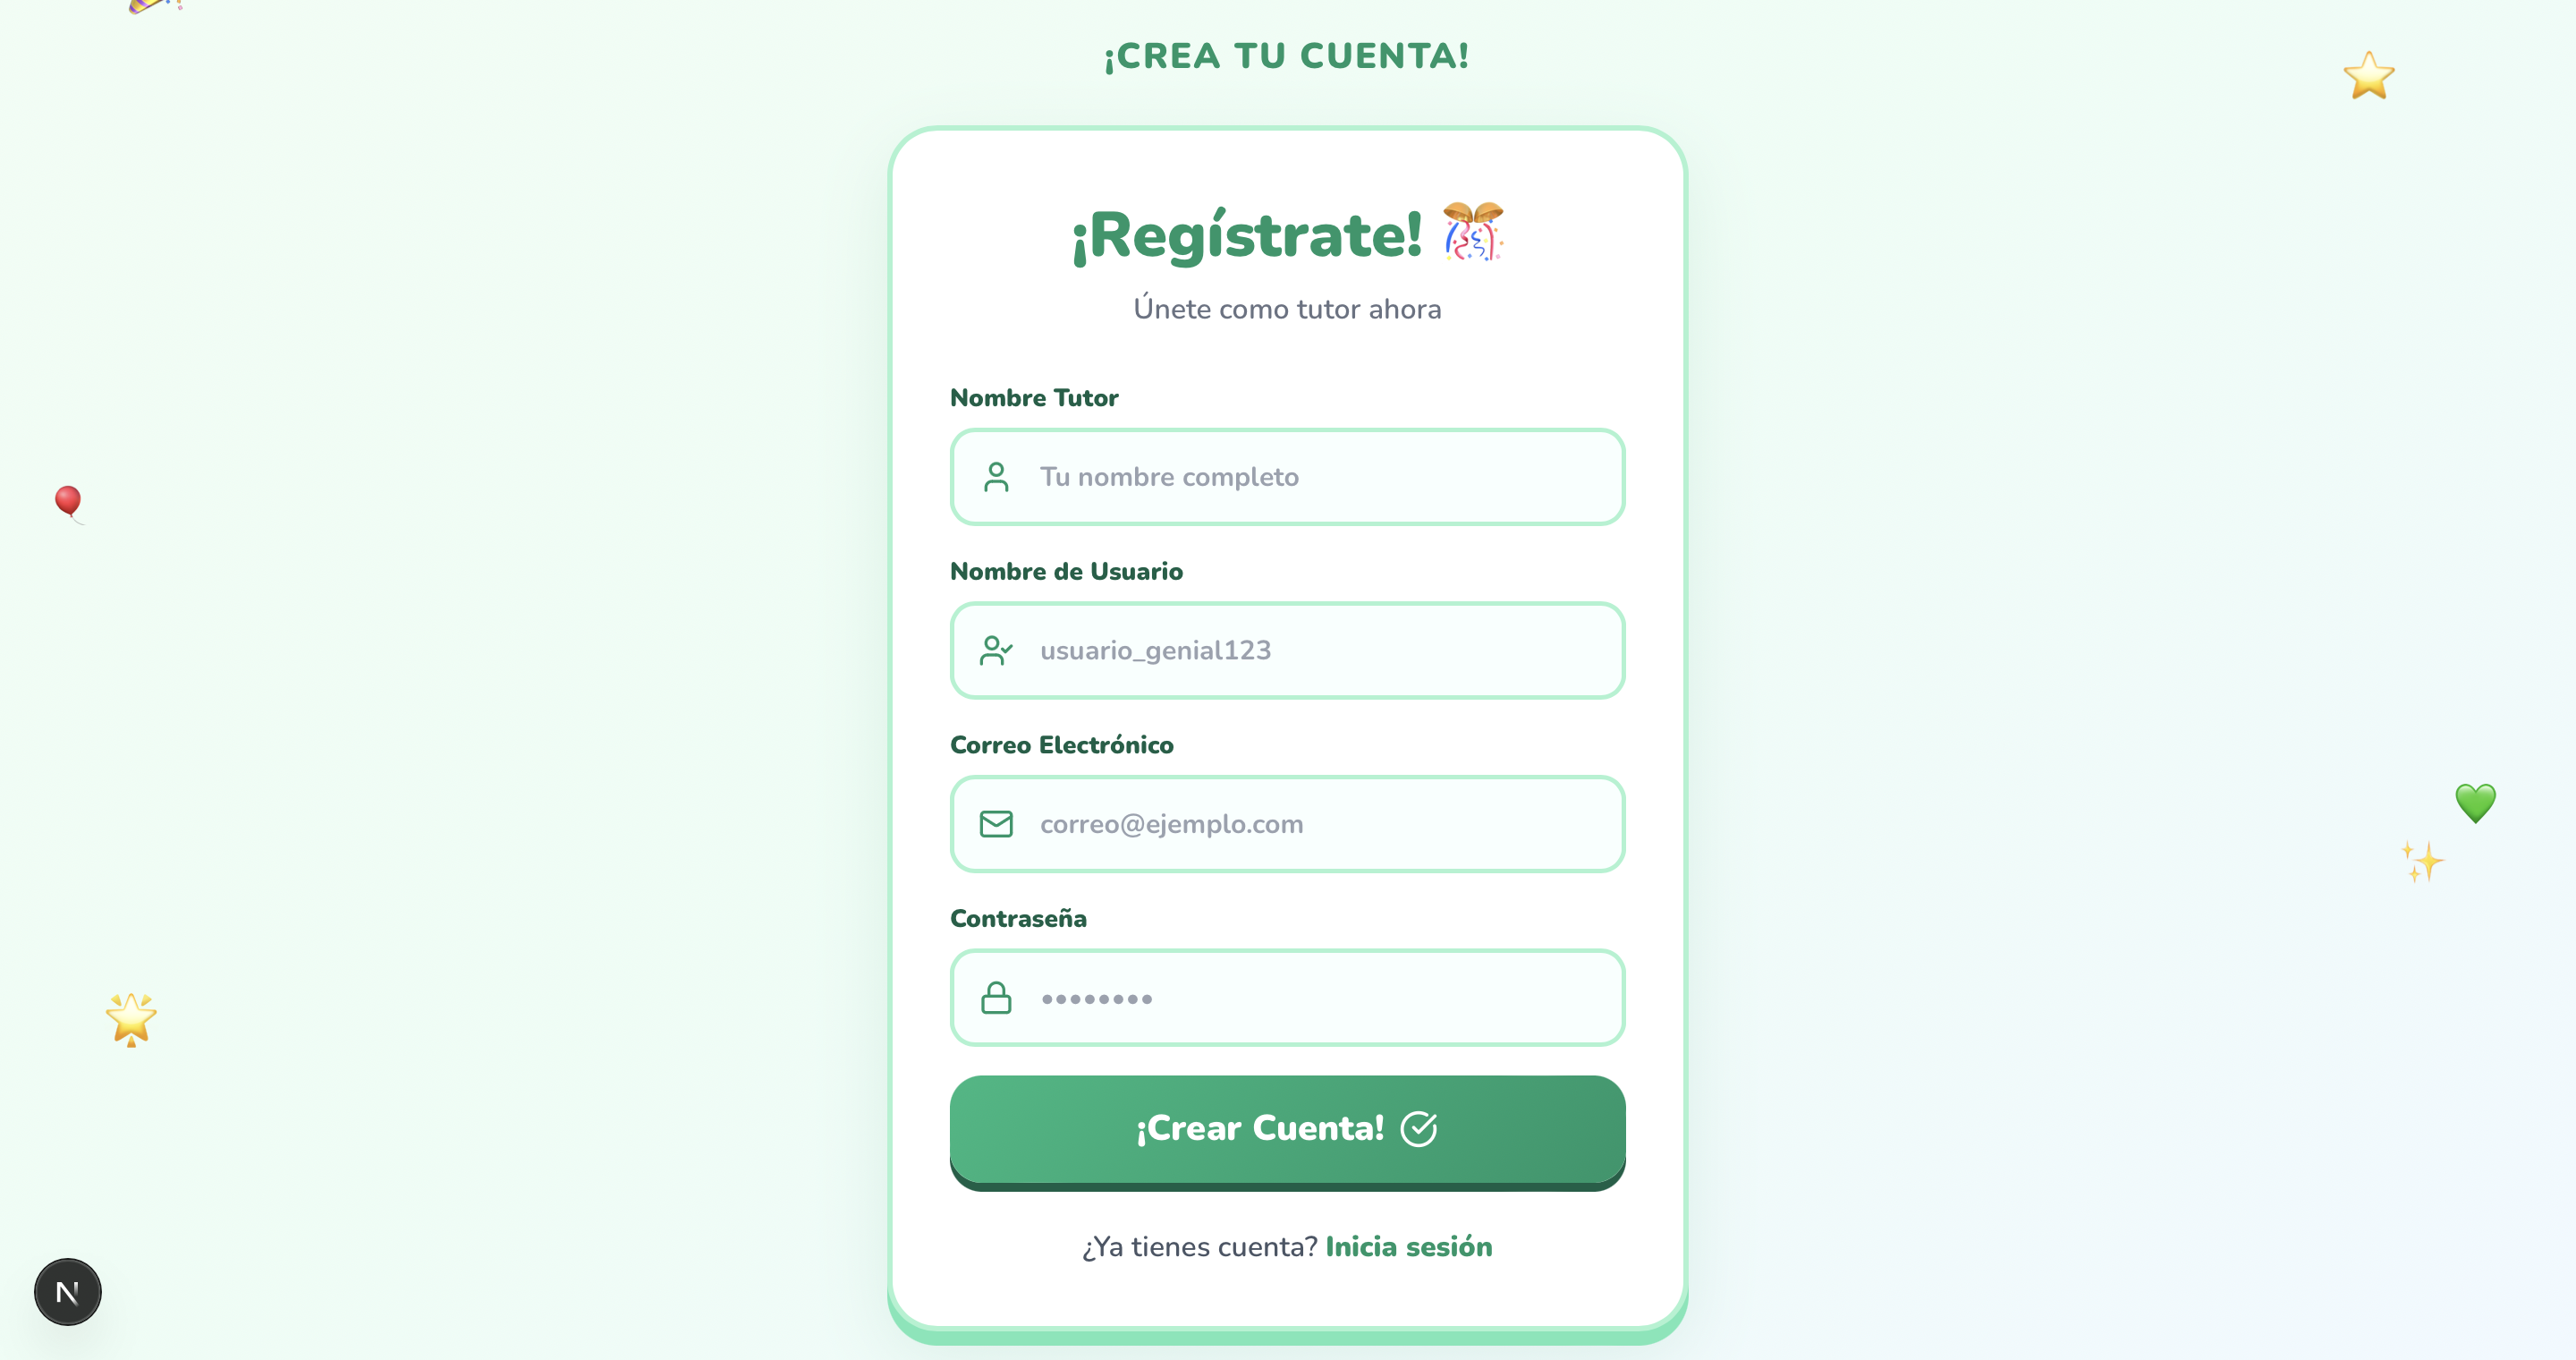
\includegraphics[width=0.7\textwidth]{Imagenes/registrar.png}
    \caption{Registro de nuevo usuario}
    \label{fig:registrar}
\end{figure}

\begin{figure}[H]
    \centering
    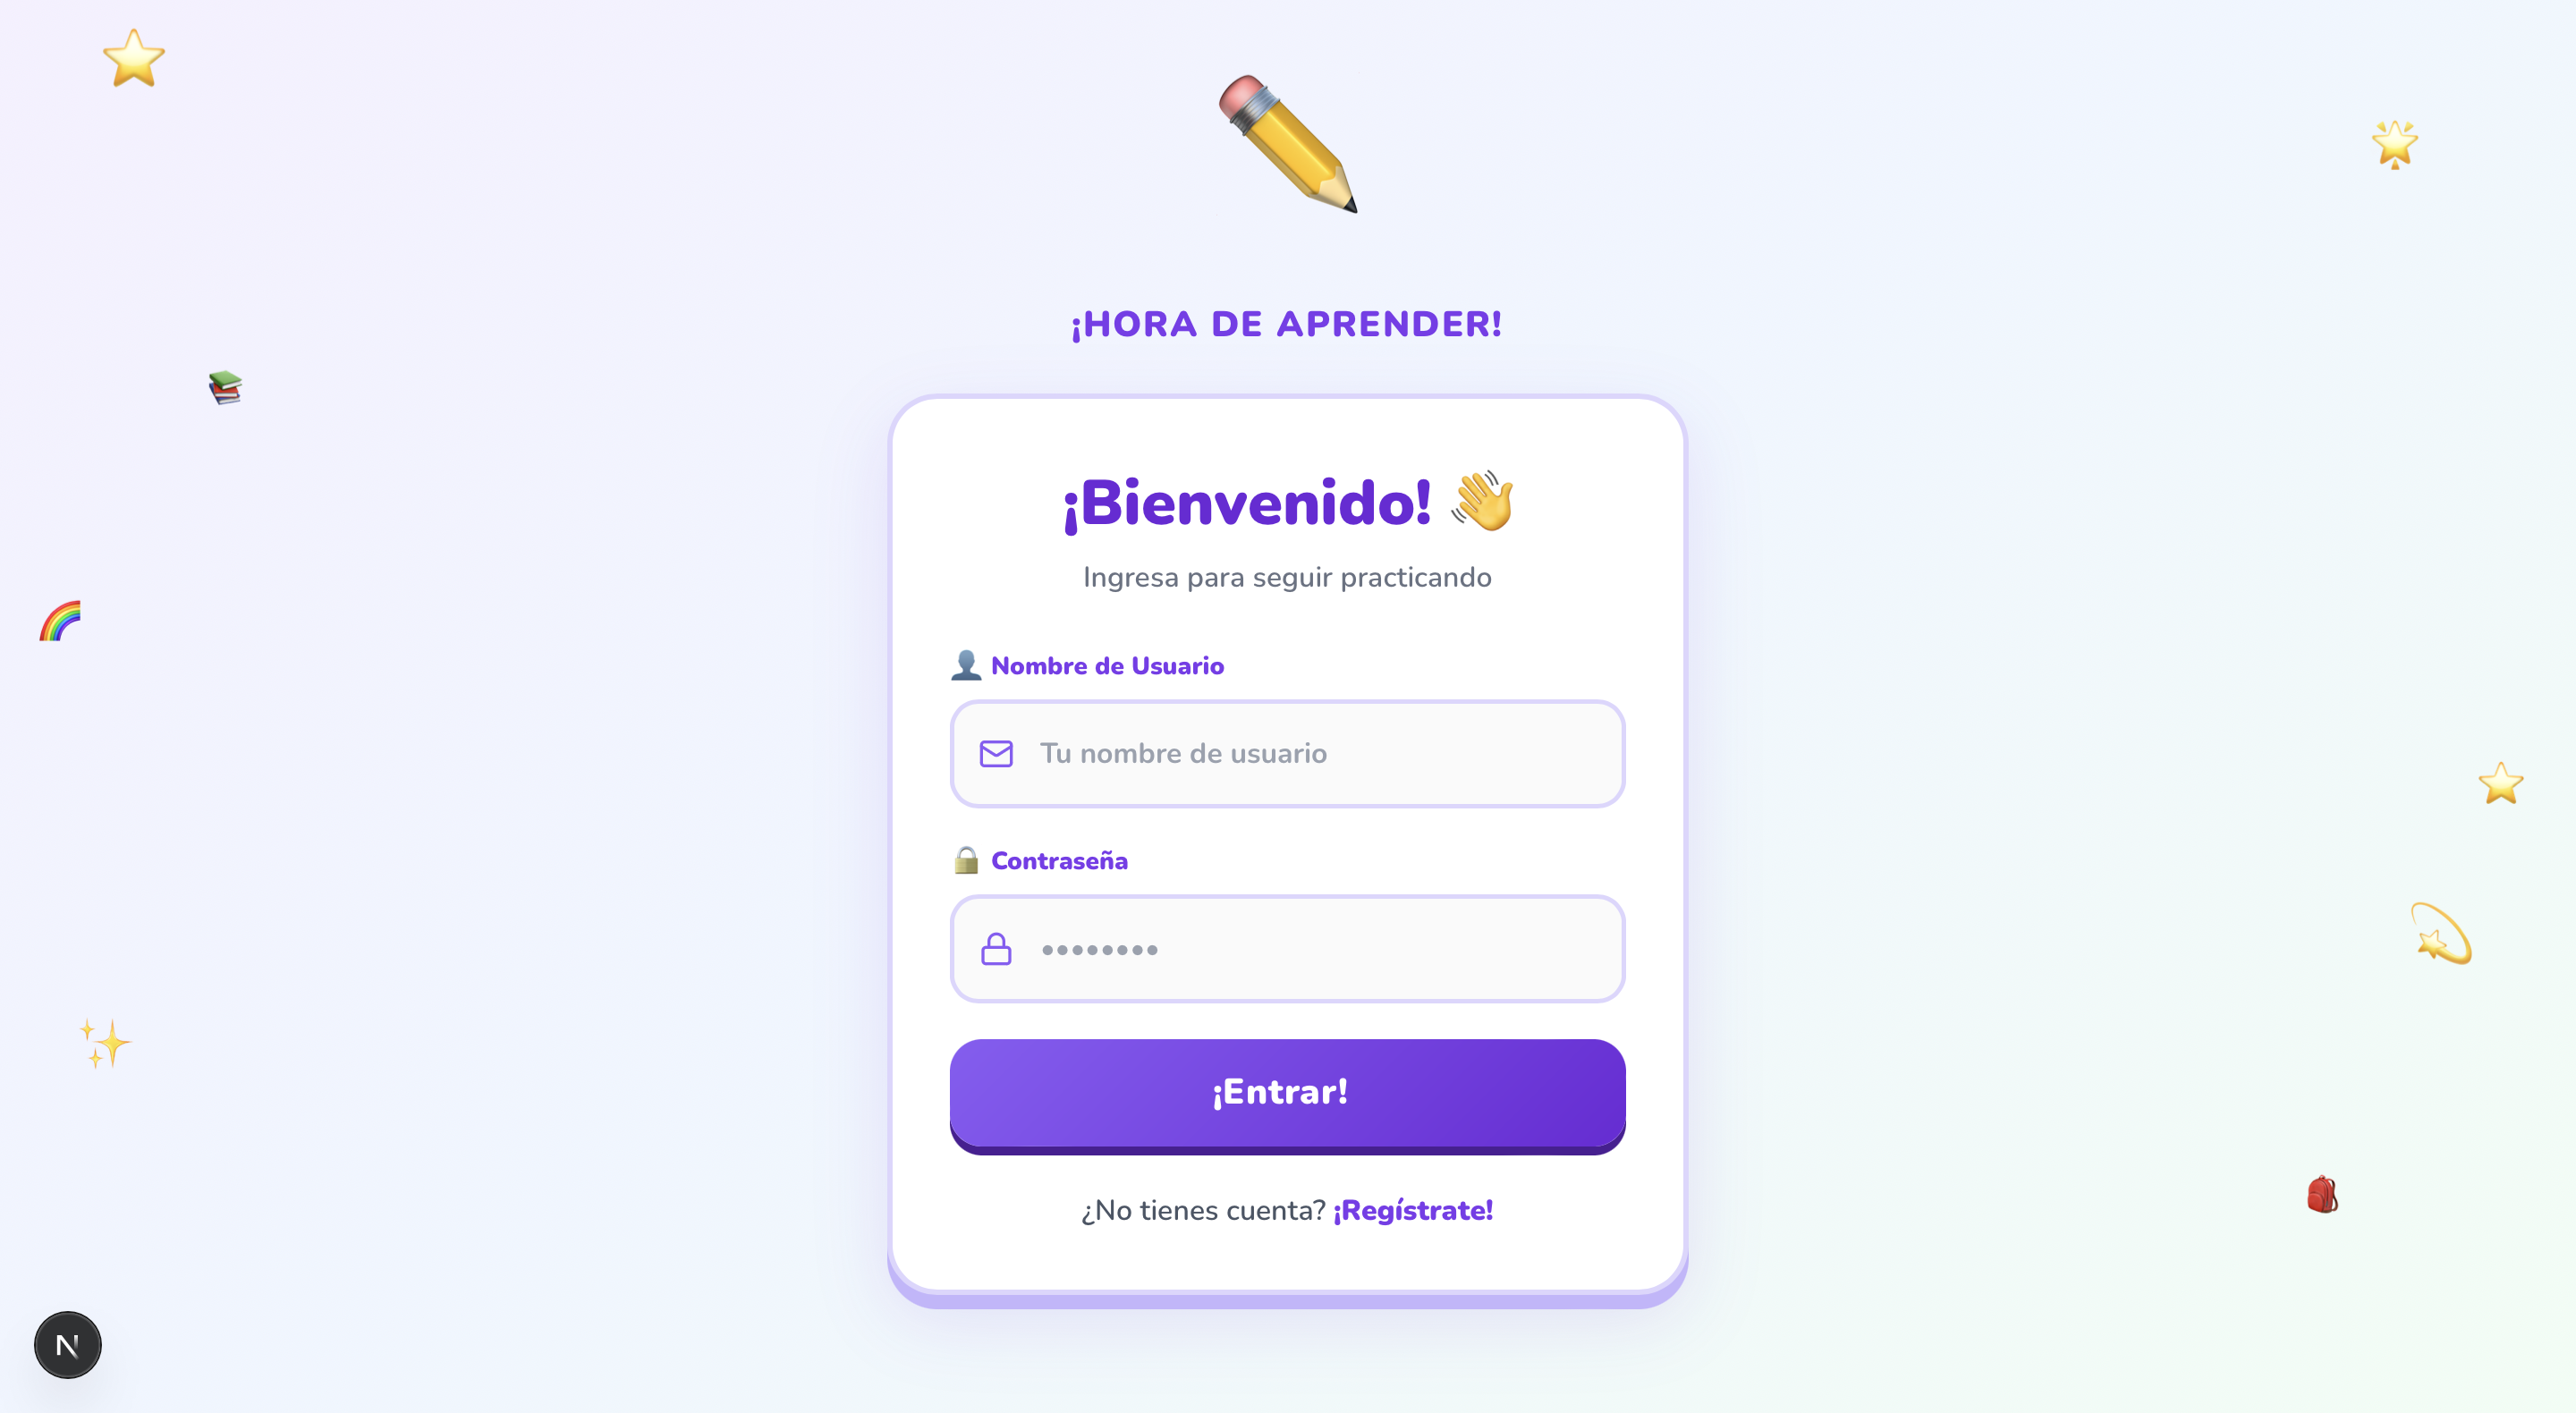
\includegraphics[width=0.7\textwidth]{Imagenes/login.png}
    \caption{Inicio de sesión}
    \label{fig:login}
\end{figure}

\subsubsection{Vistas del tutor}

\begin{figure}[H]
    \centering
    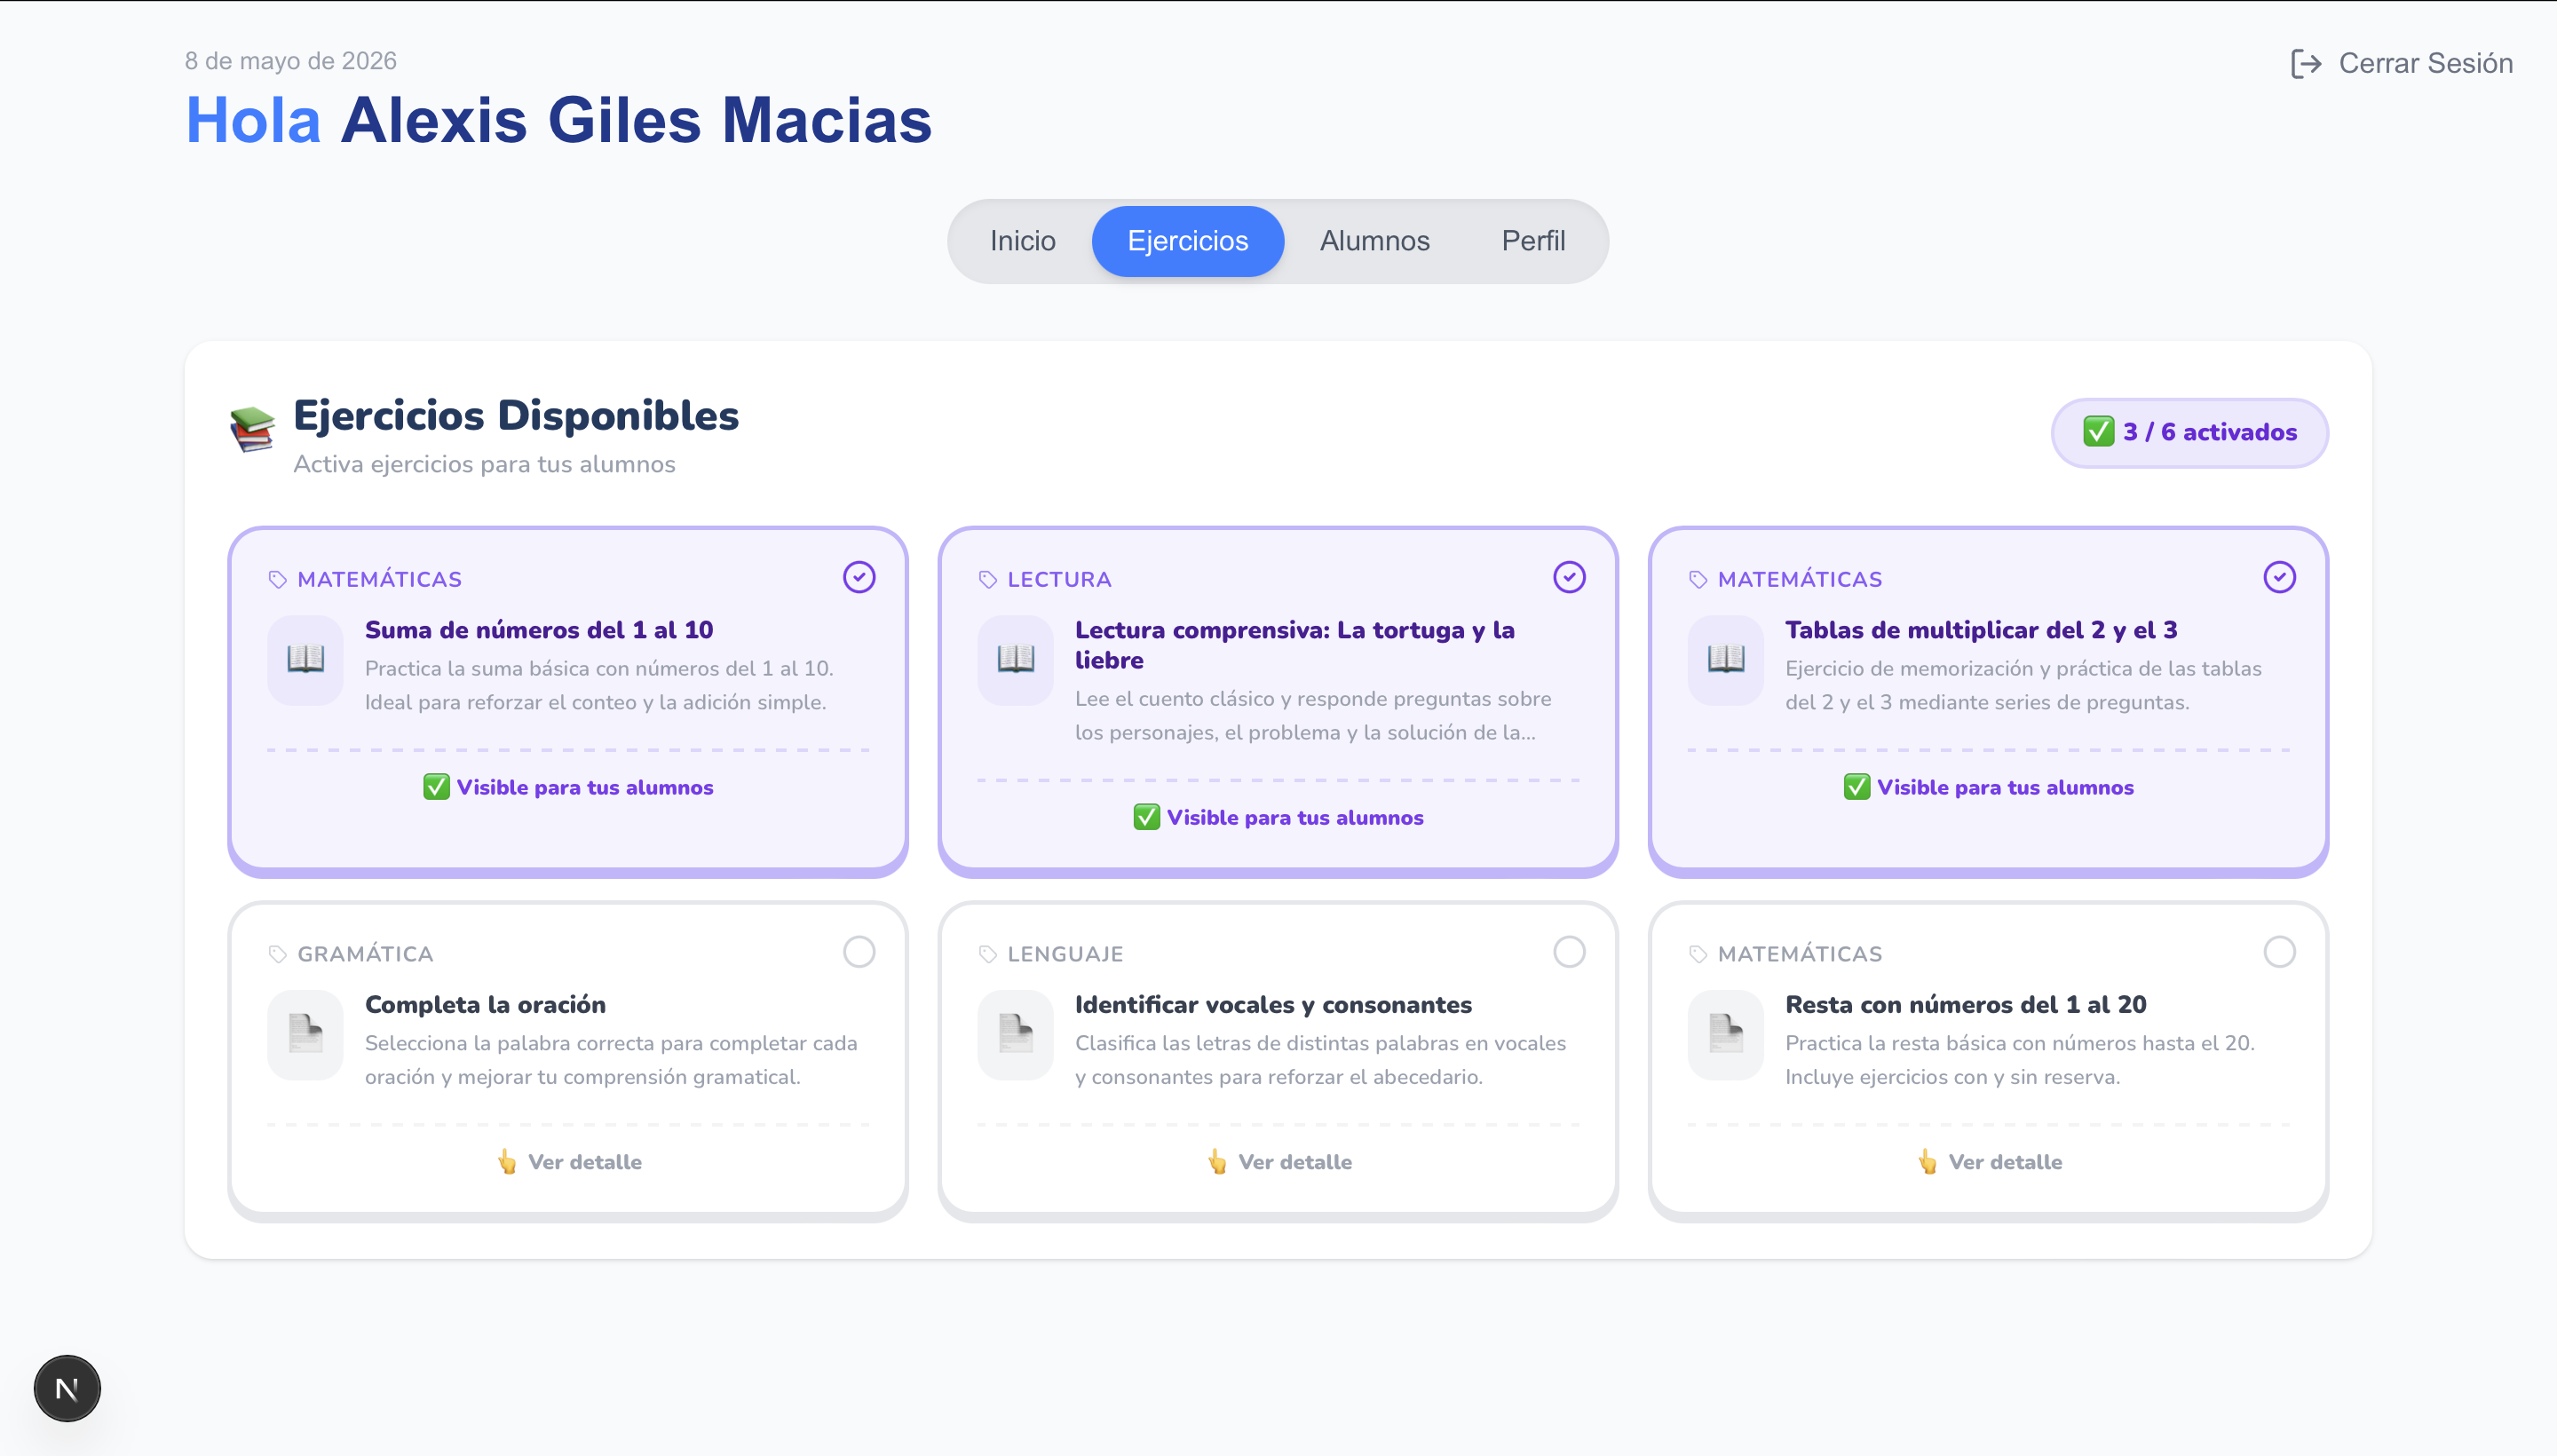
\includegraphics[width=0.7\textwidth]{Imagenes/EjerciciosTutor.png}
    \caption{Catalogo de ejercicios para tutor y ejercicios}
    \label{fig:ejeTu}
\end{figure}

\begin{figure}[H]
    \centering
    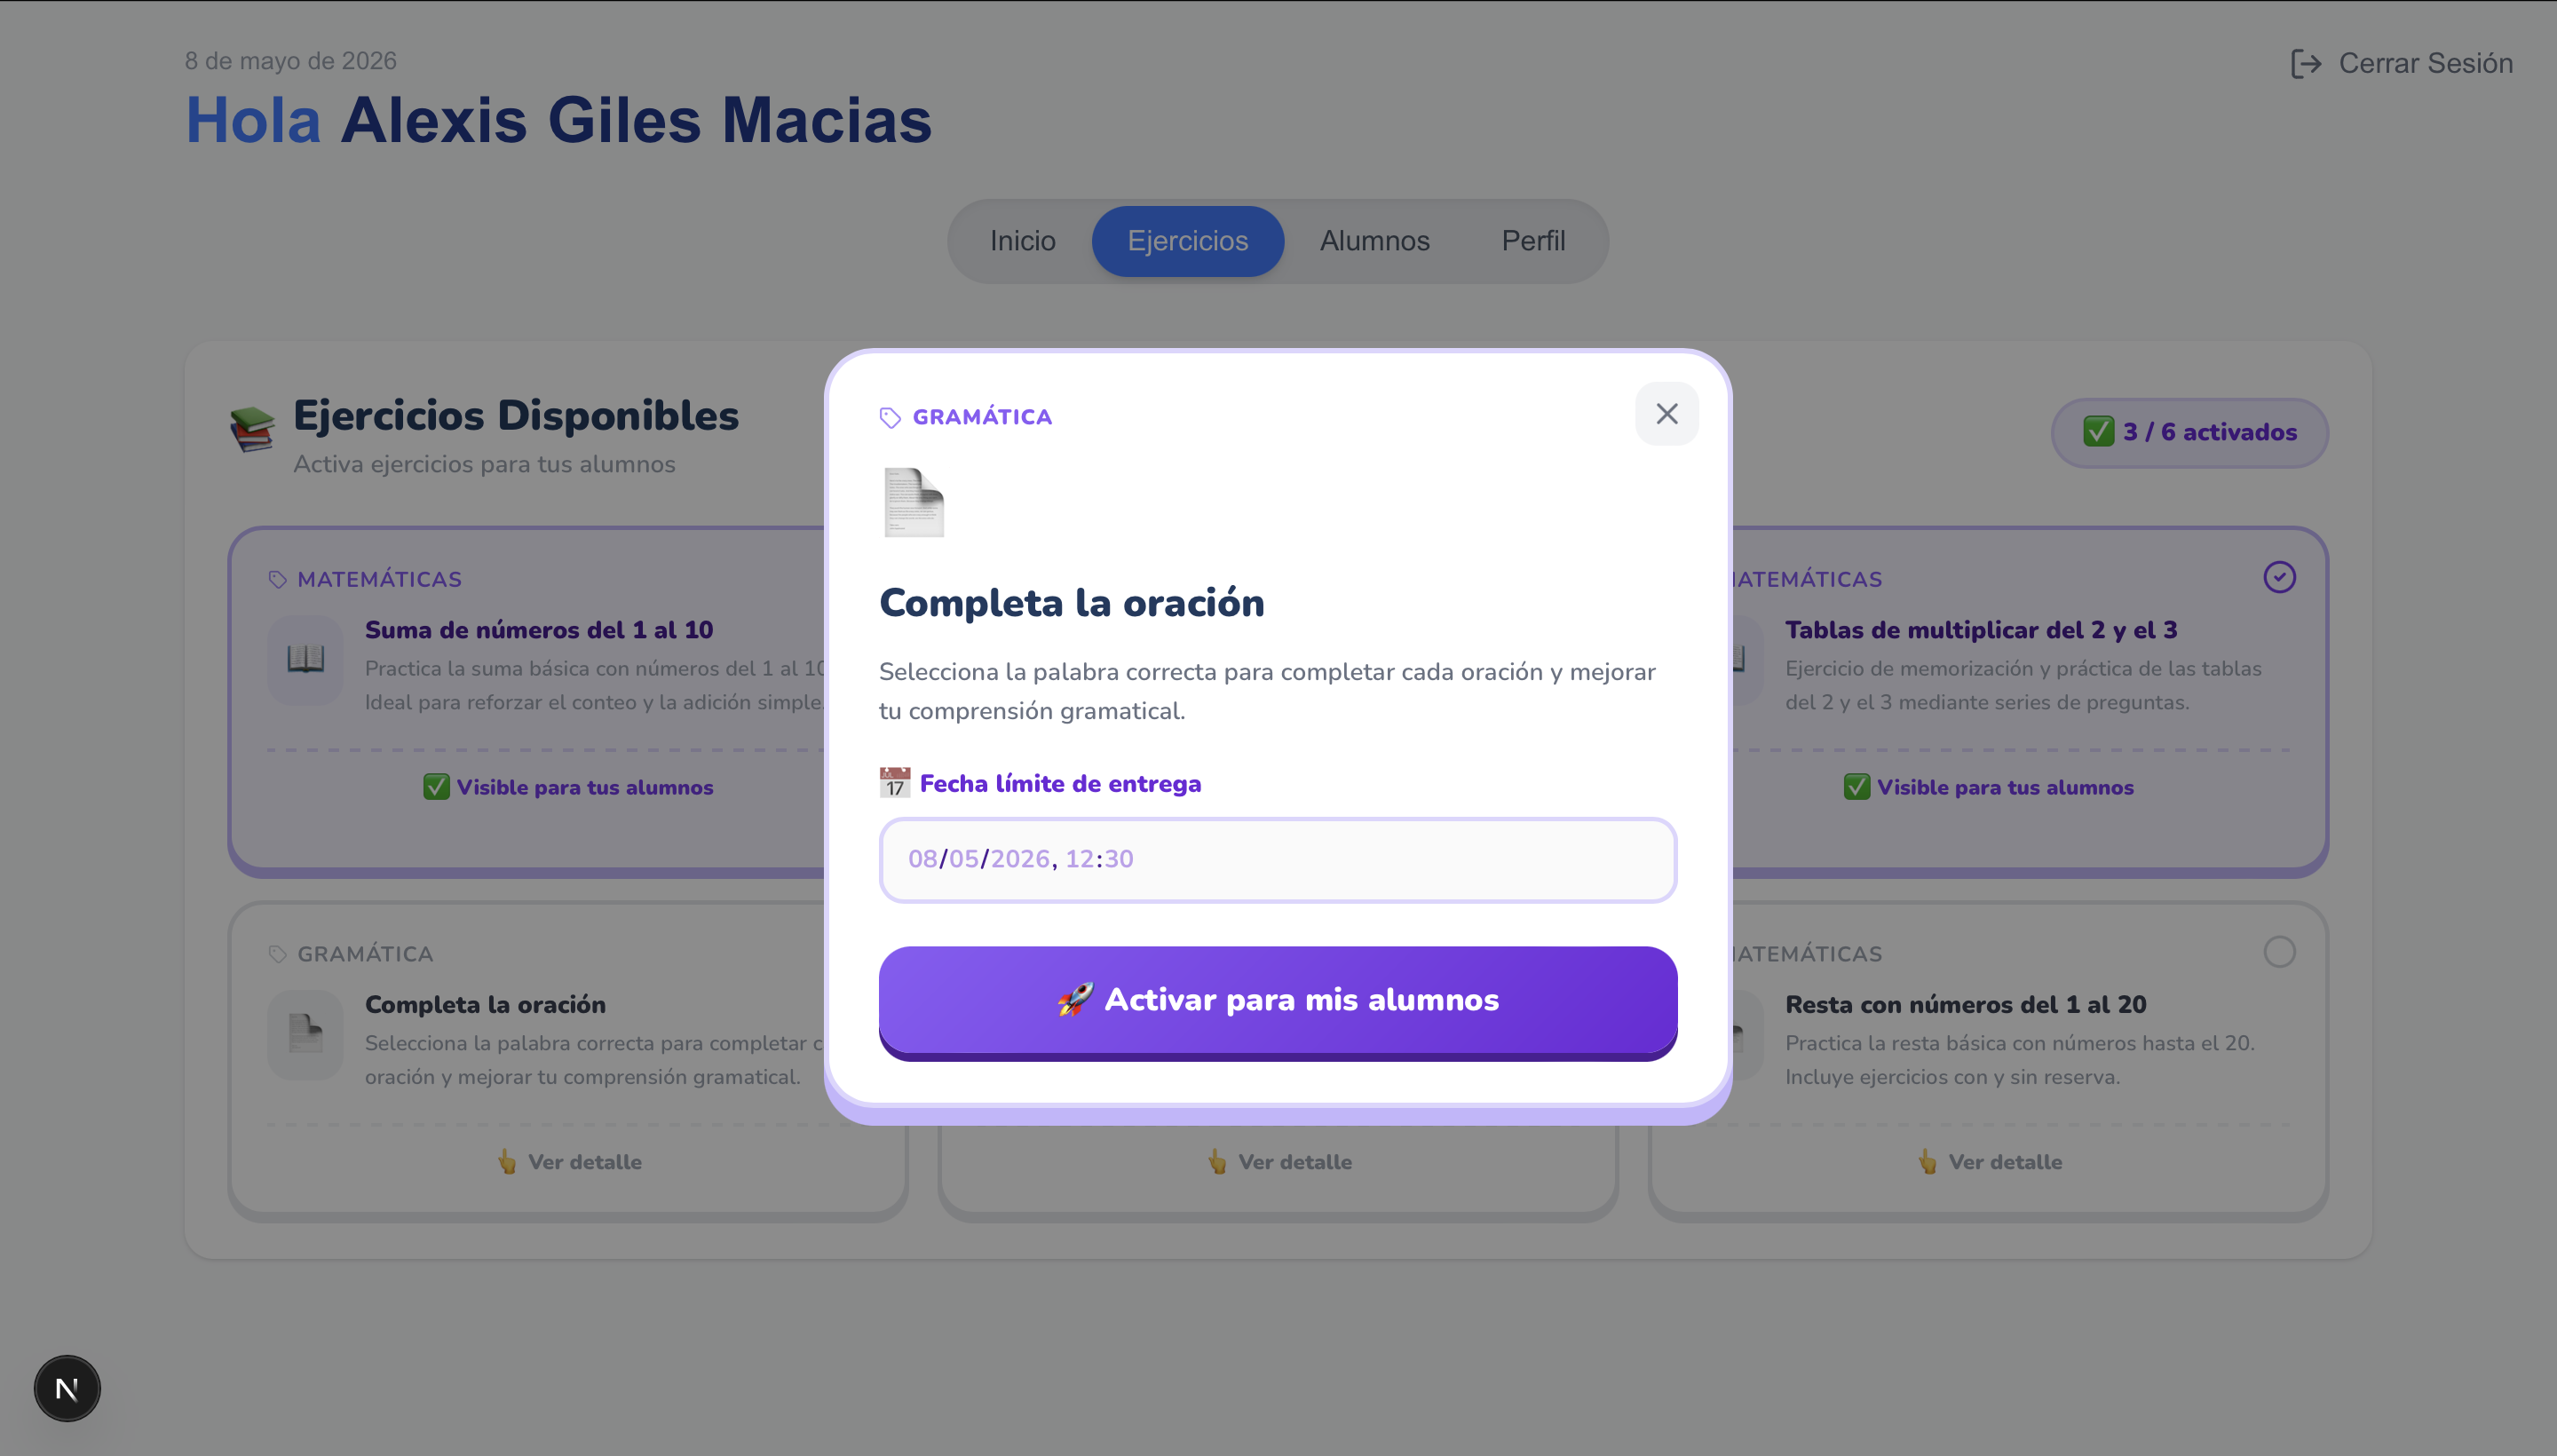
\includegraphics[width=0.7\textwidth]{Imagenes/asignacion.png}
    \caption{Asignacion de ejercicios a alumnos}
    \label{fig:asignacionEje}
\end{figure}

\begin{figure}[H]
    \centering
    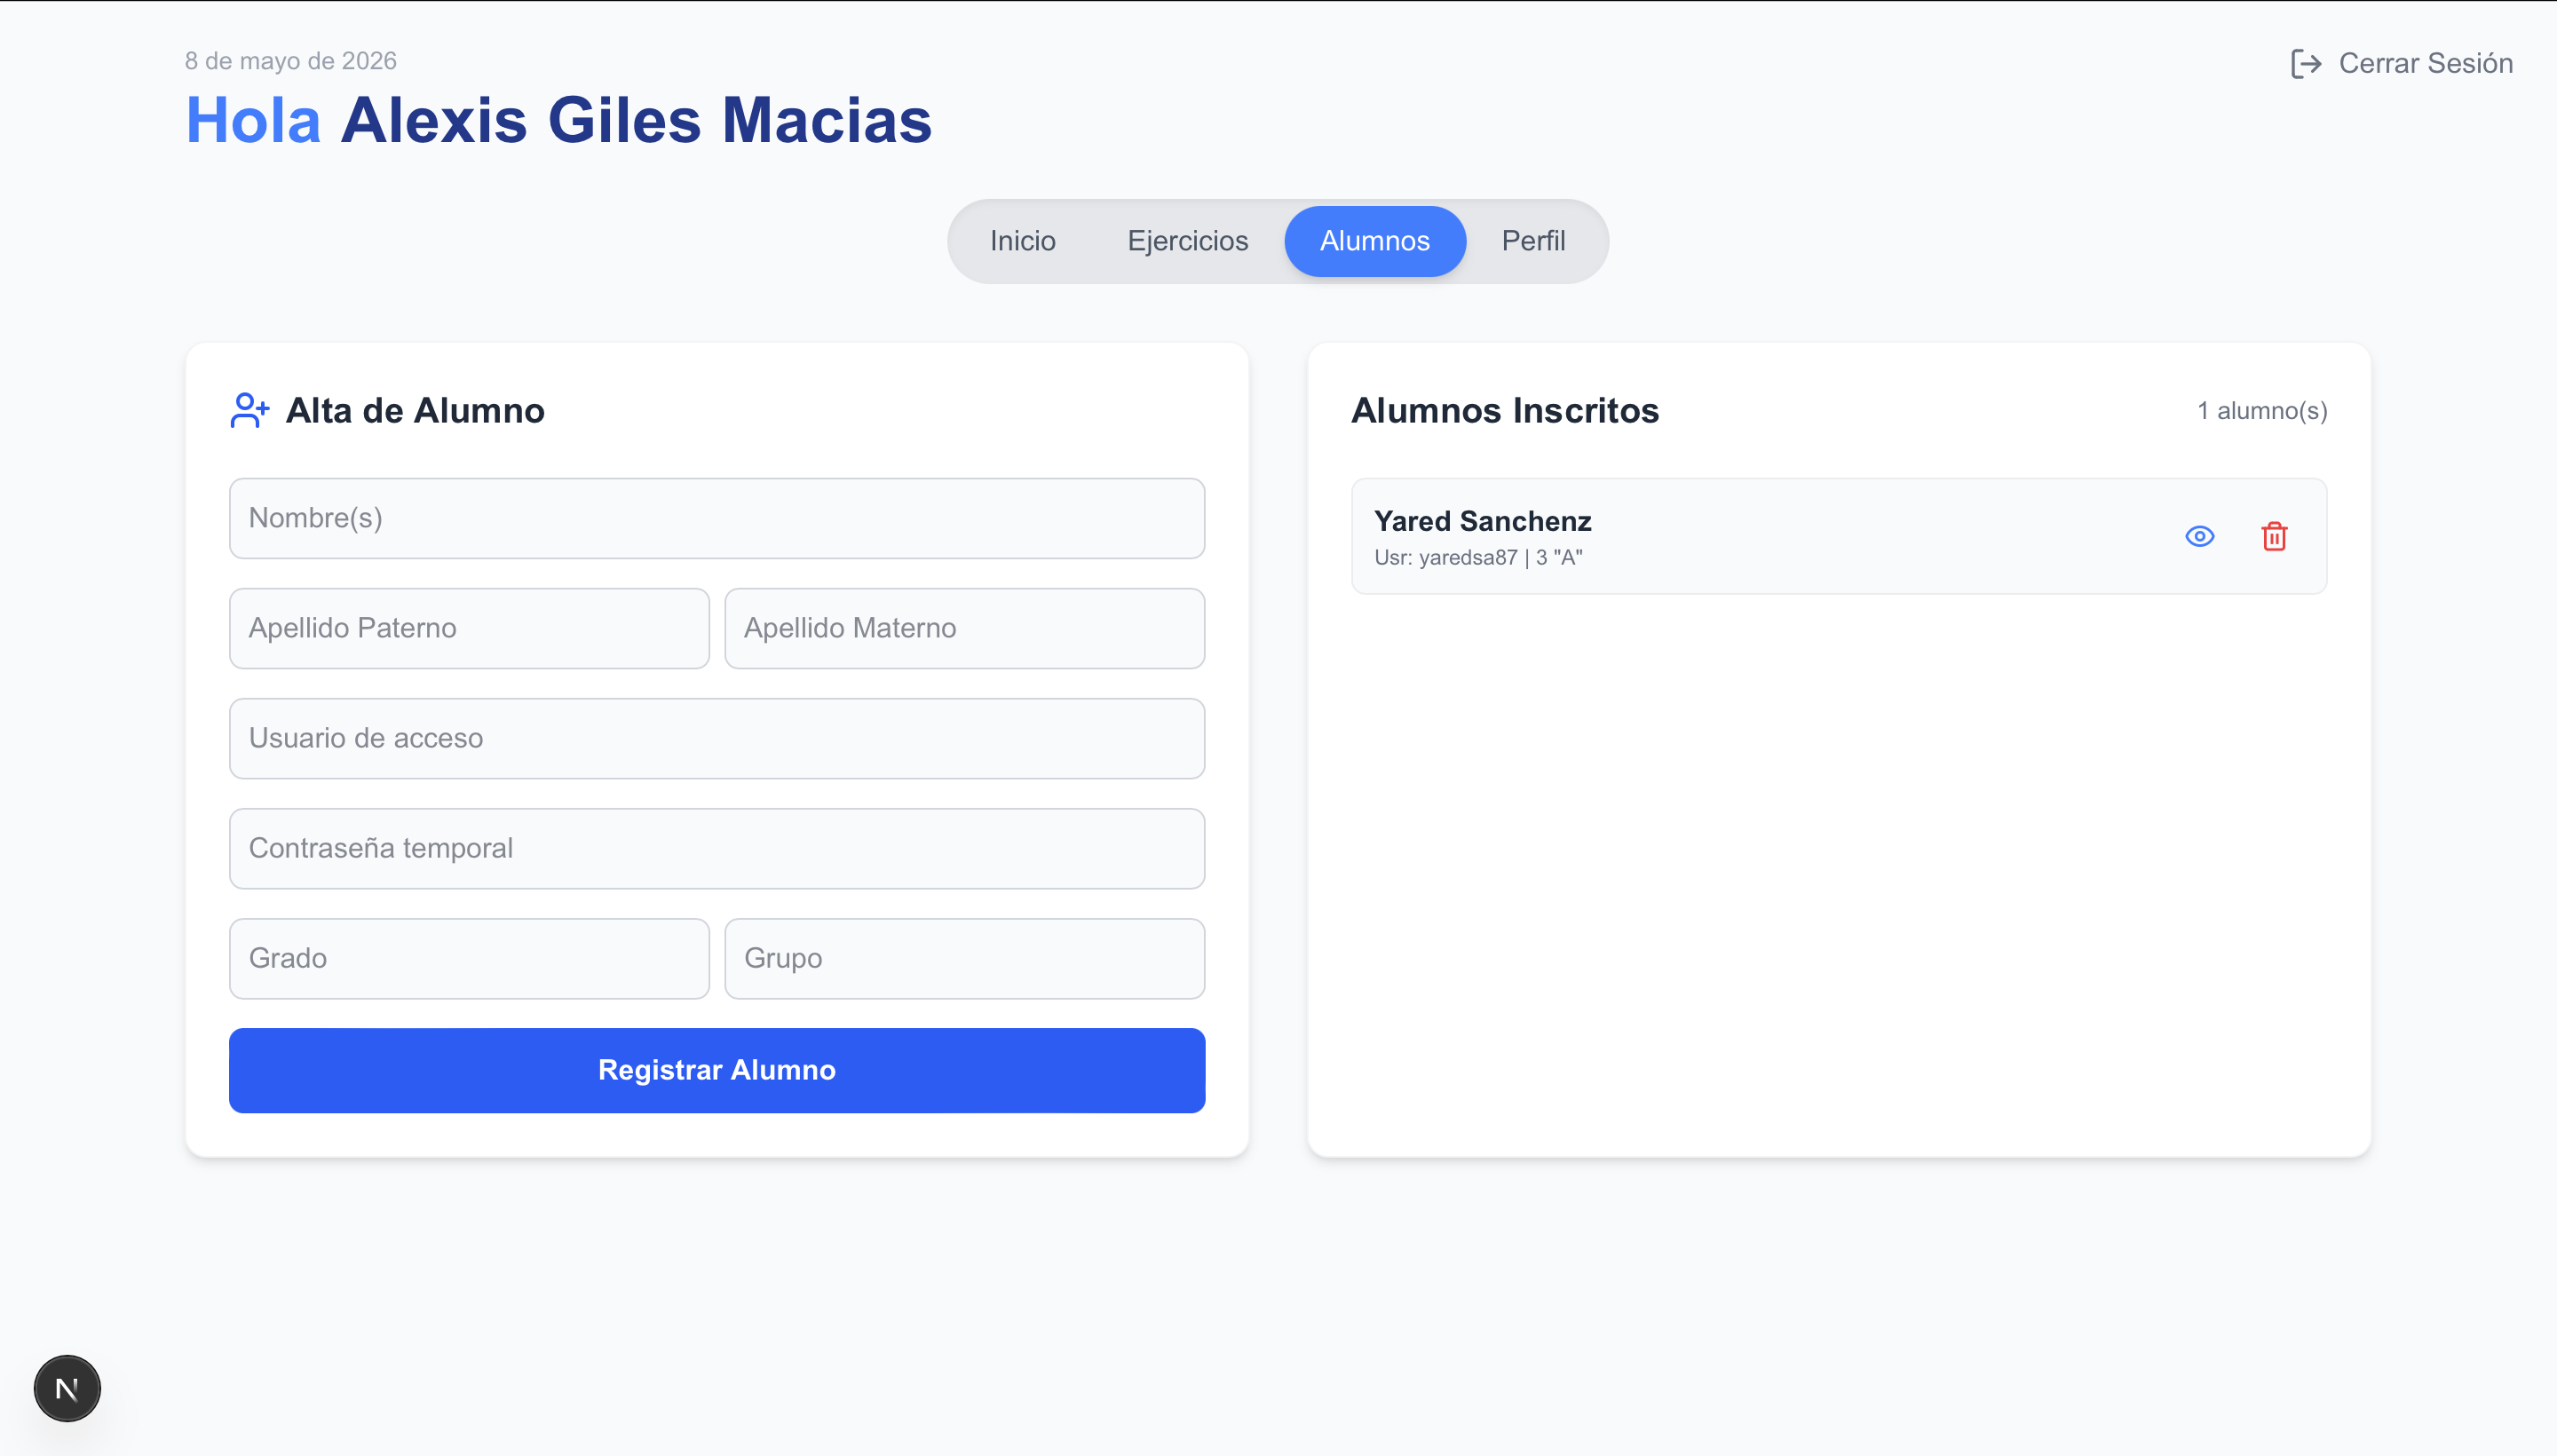
\includegraphics[width=0.7\textwidth]{Imagenes/AlumnosInscritos.png}
    \caption{Alta de alumnos y visualización de alumnos inscritos}
    \label{fig:alumnosInscritos}
\end{figure}

\begin{figure}[H]
    \centering
    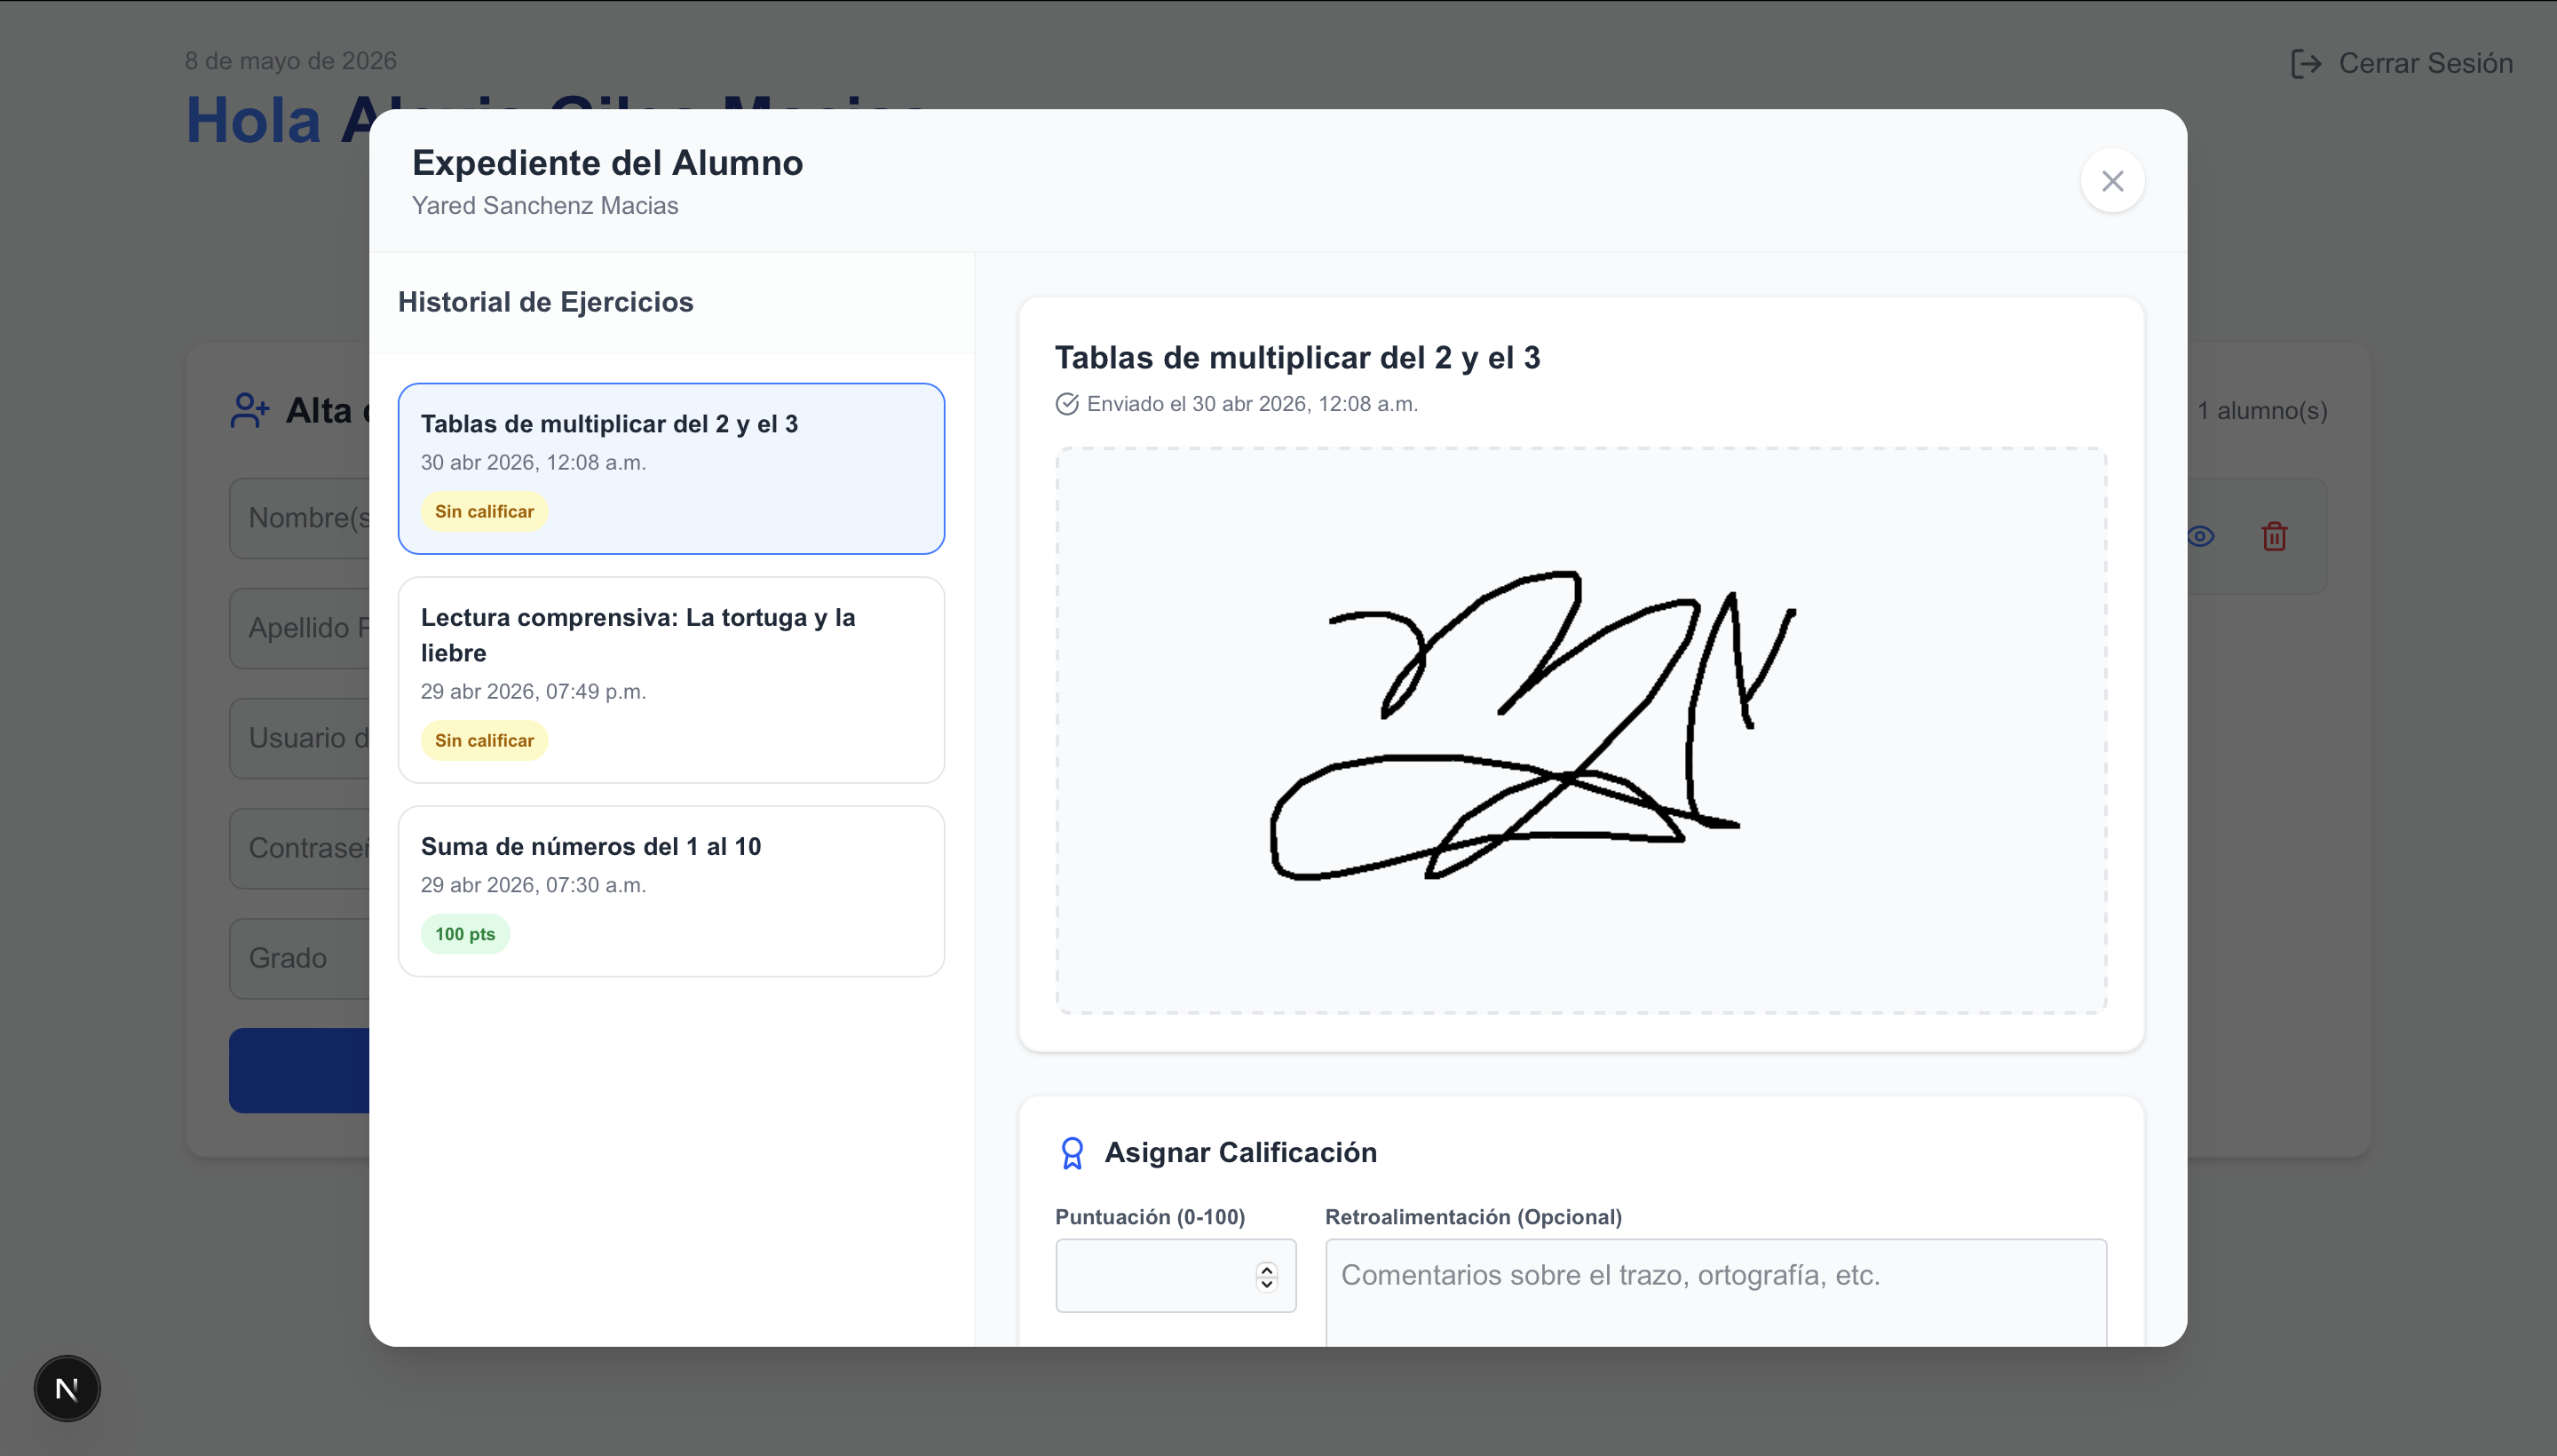
\includegraphics[width=0.7\textwidth]{Imagenes/historialAlumnos.png}
    \caption{Visualizacion del historial de ejercicios realizados por los alumnos}
    \label{fig:historialAlumnos}
\end{figure}

\begin{figure}[H]
    \centering
    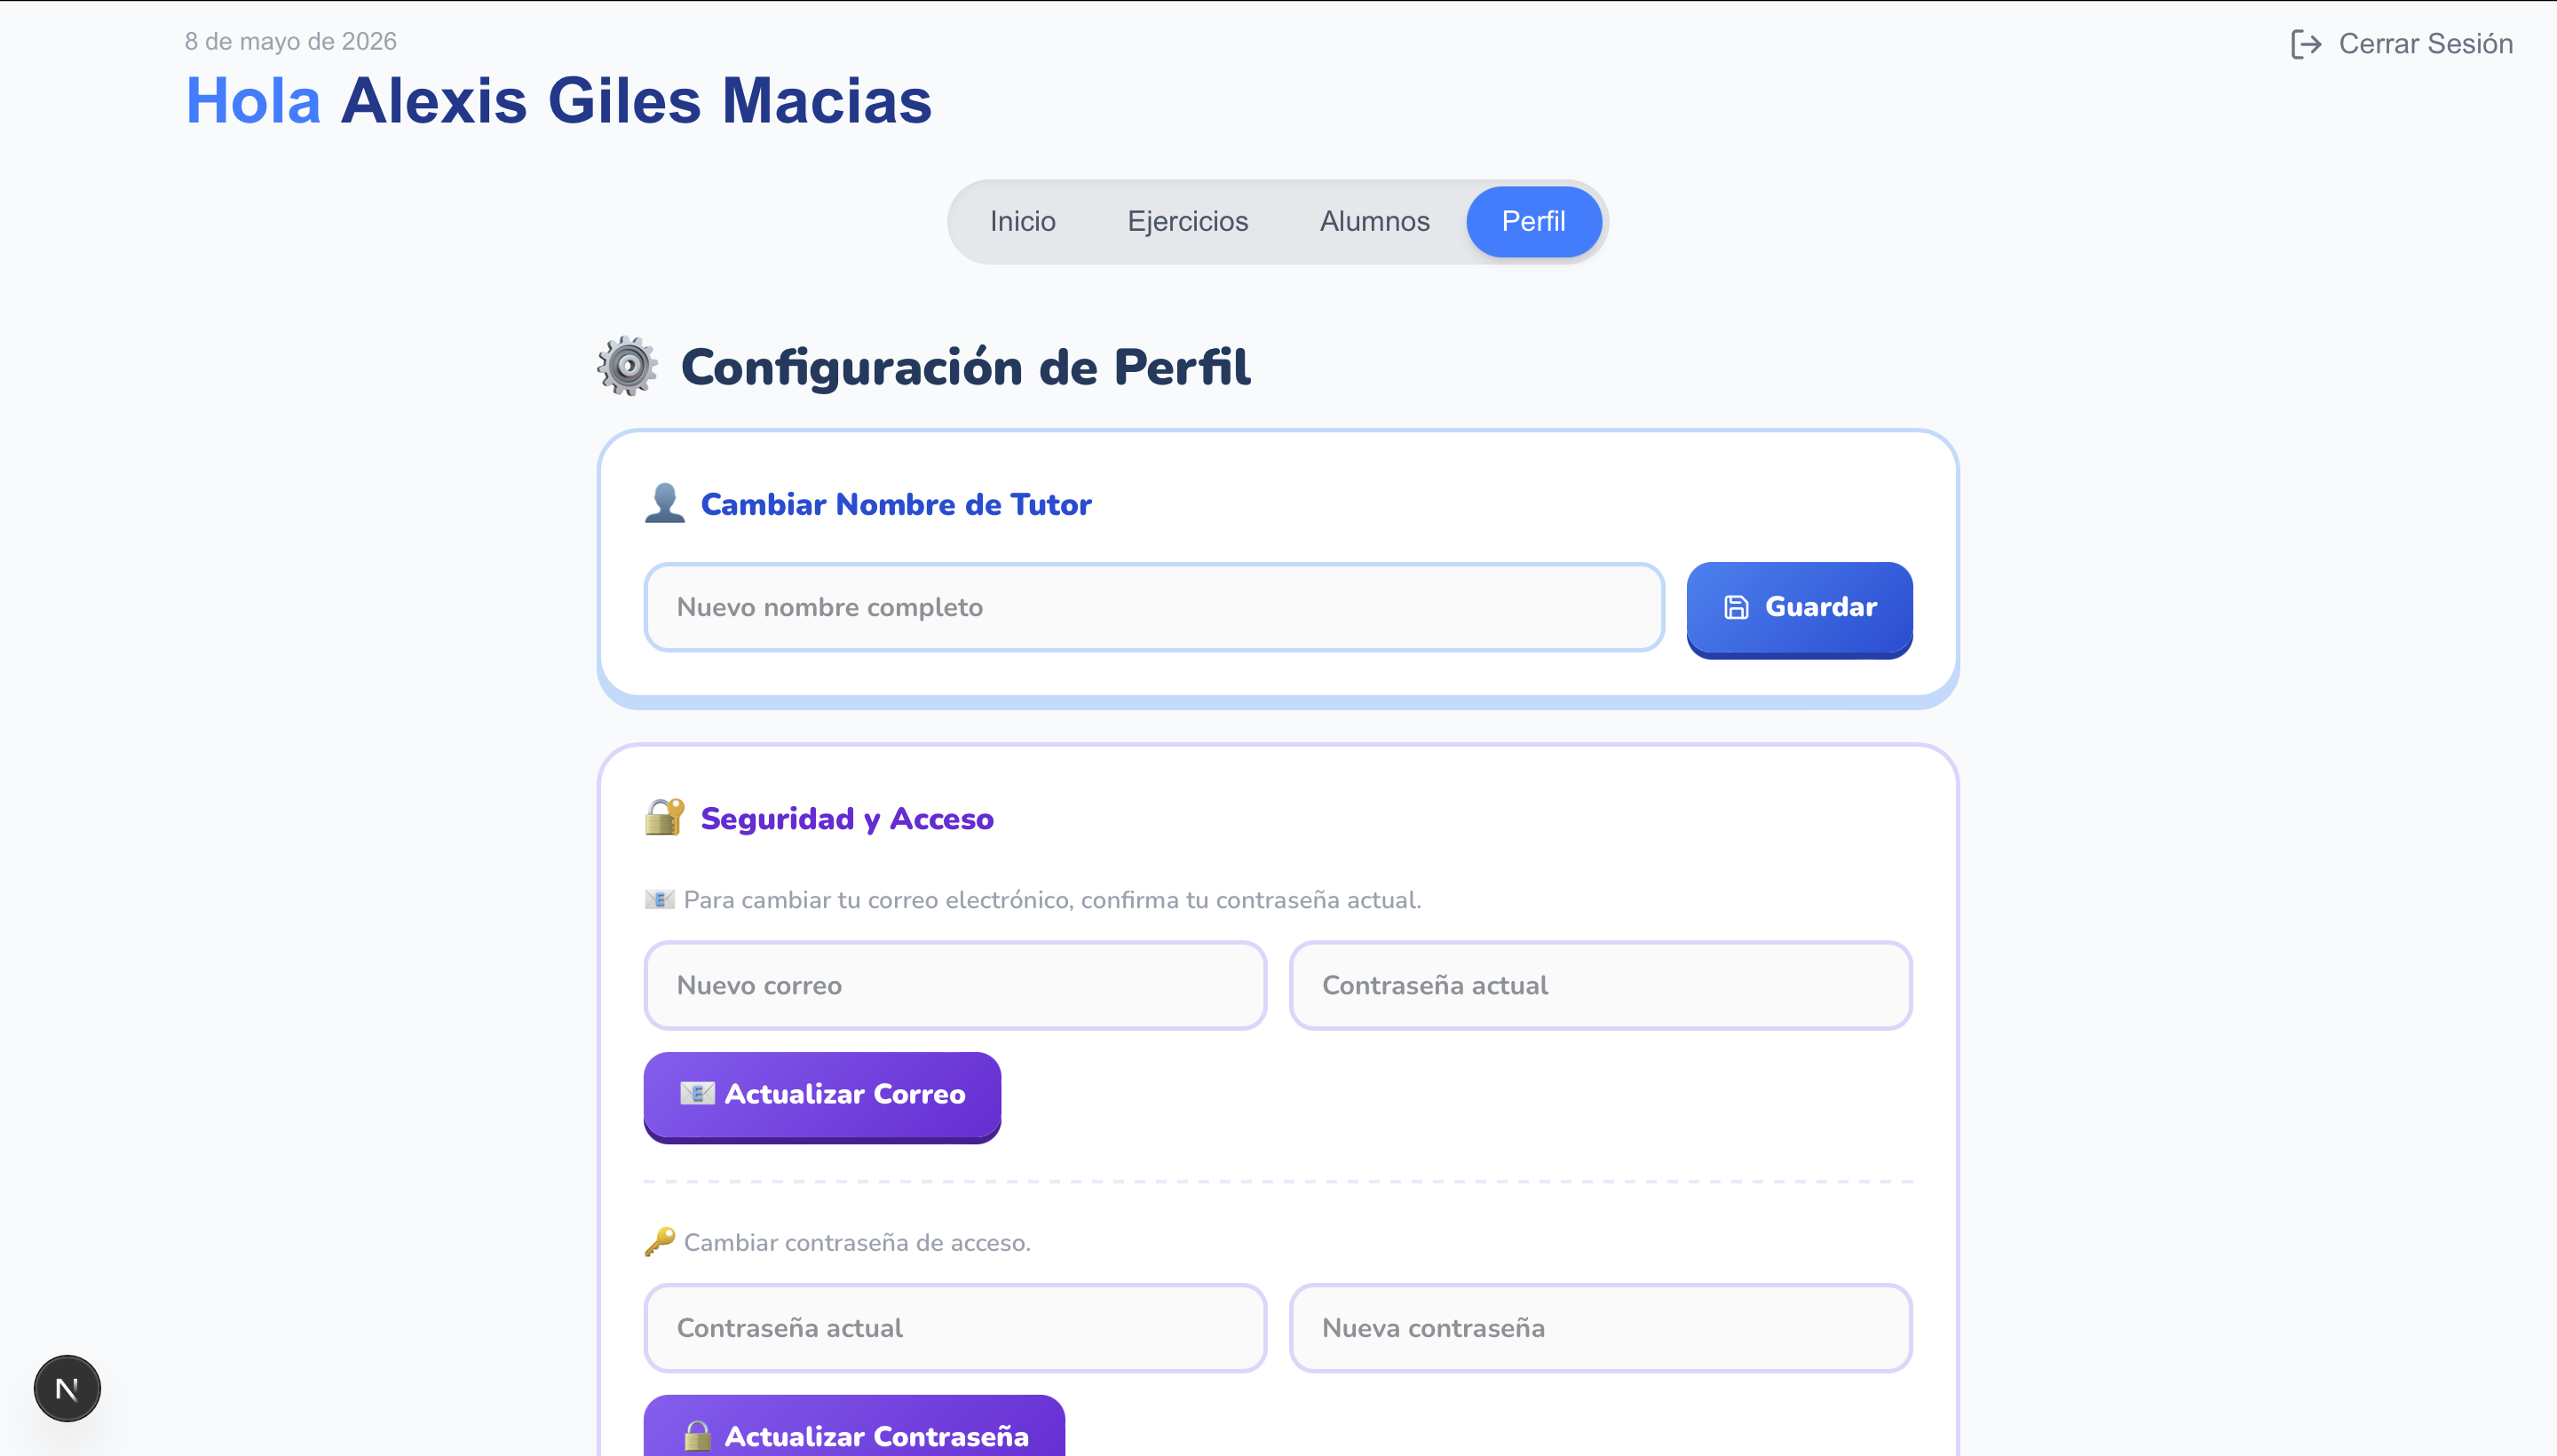
\includegraphics[width=0.7\textwidth]{Imagenes/miperfil.png}
    \caption{Visualizacion del perfil del tutor}
    \label{fig:miperfilT}
\end{figure}

\subsubsection{Vistas del alumno}

\begin{figure}[H]
    \centering
    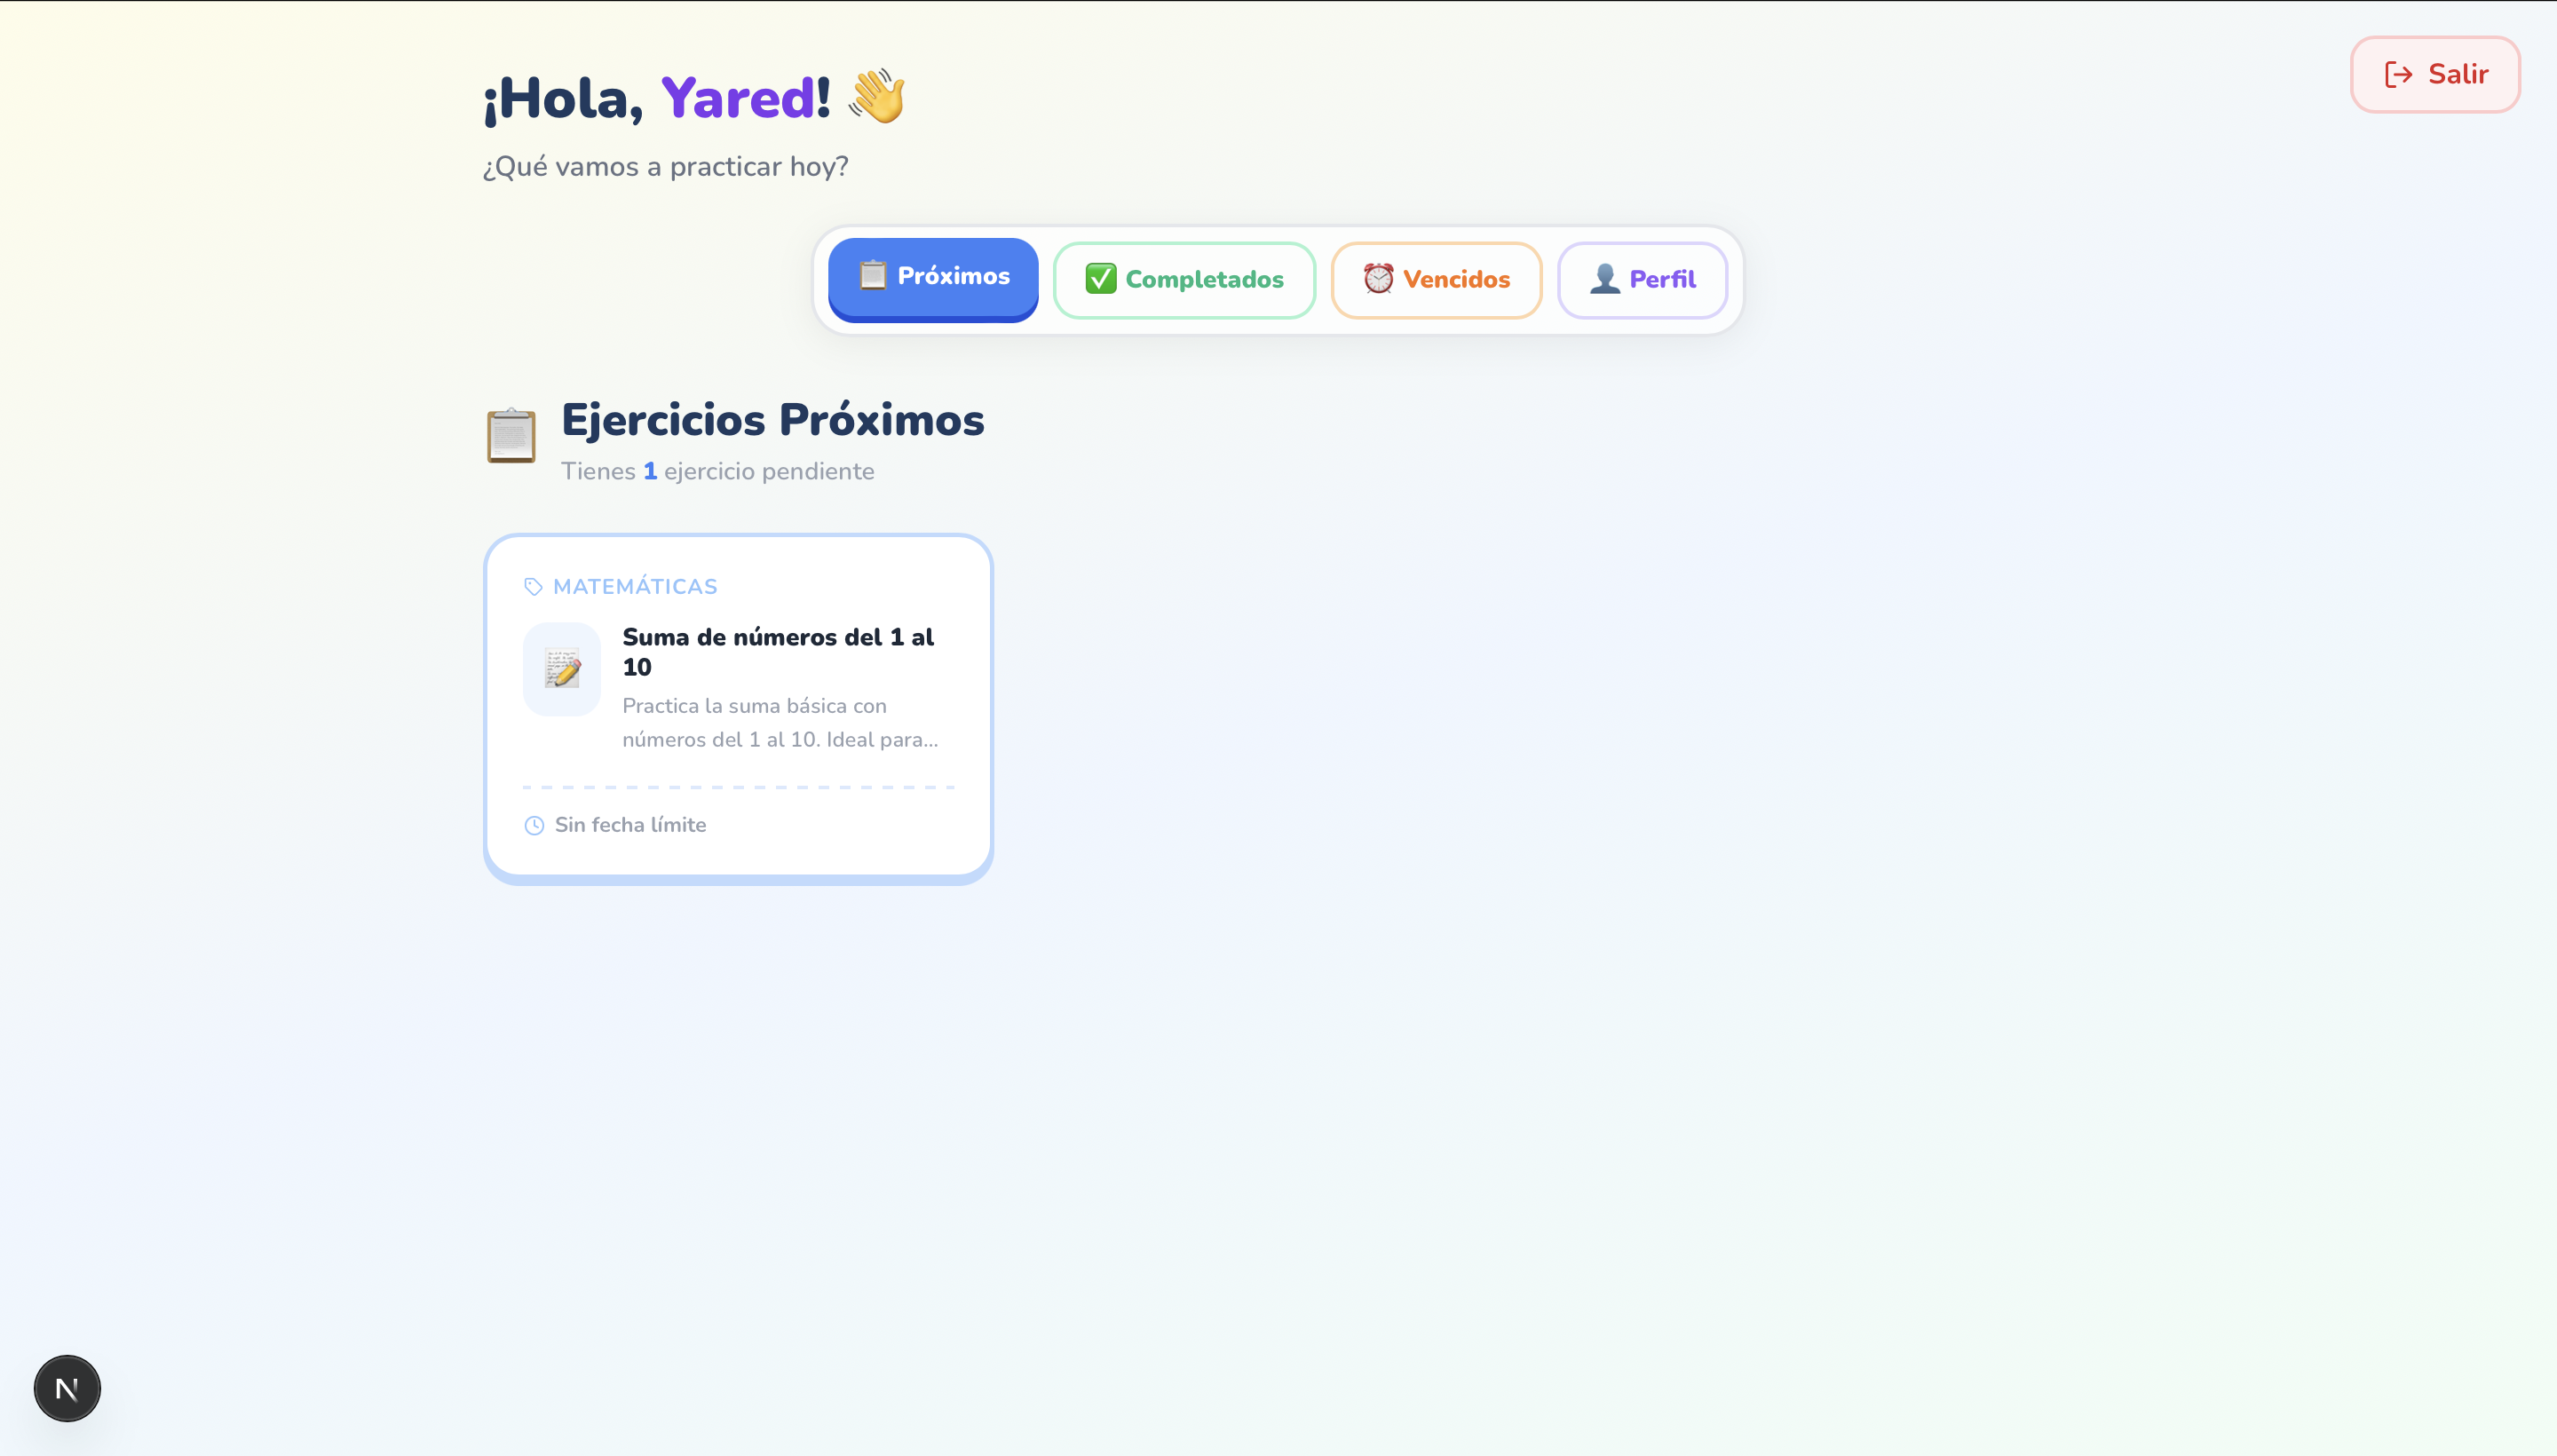
\includegraphics[width=0.7\textwidth]{Imagenes/ejerciciosProximos.png}
    \caption{Visualización de ejercicios próximos a vencer}
    \label{fig:ejerciciosProximos}
\end{figure}

\begin{figure}[H]
    \centering
    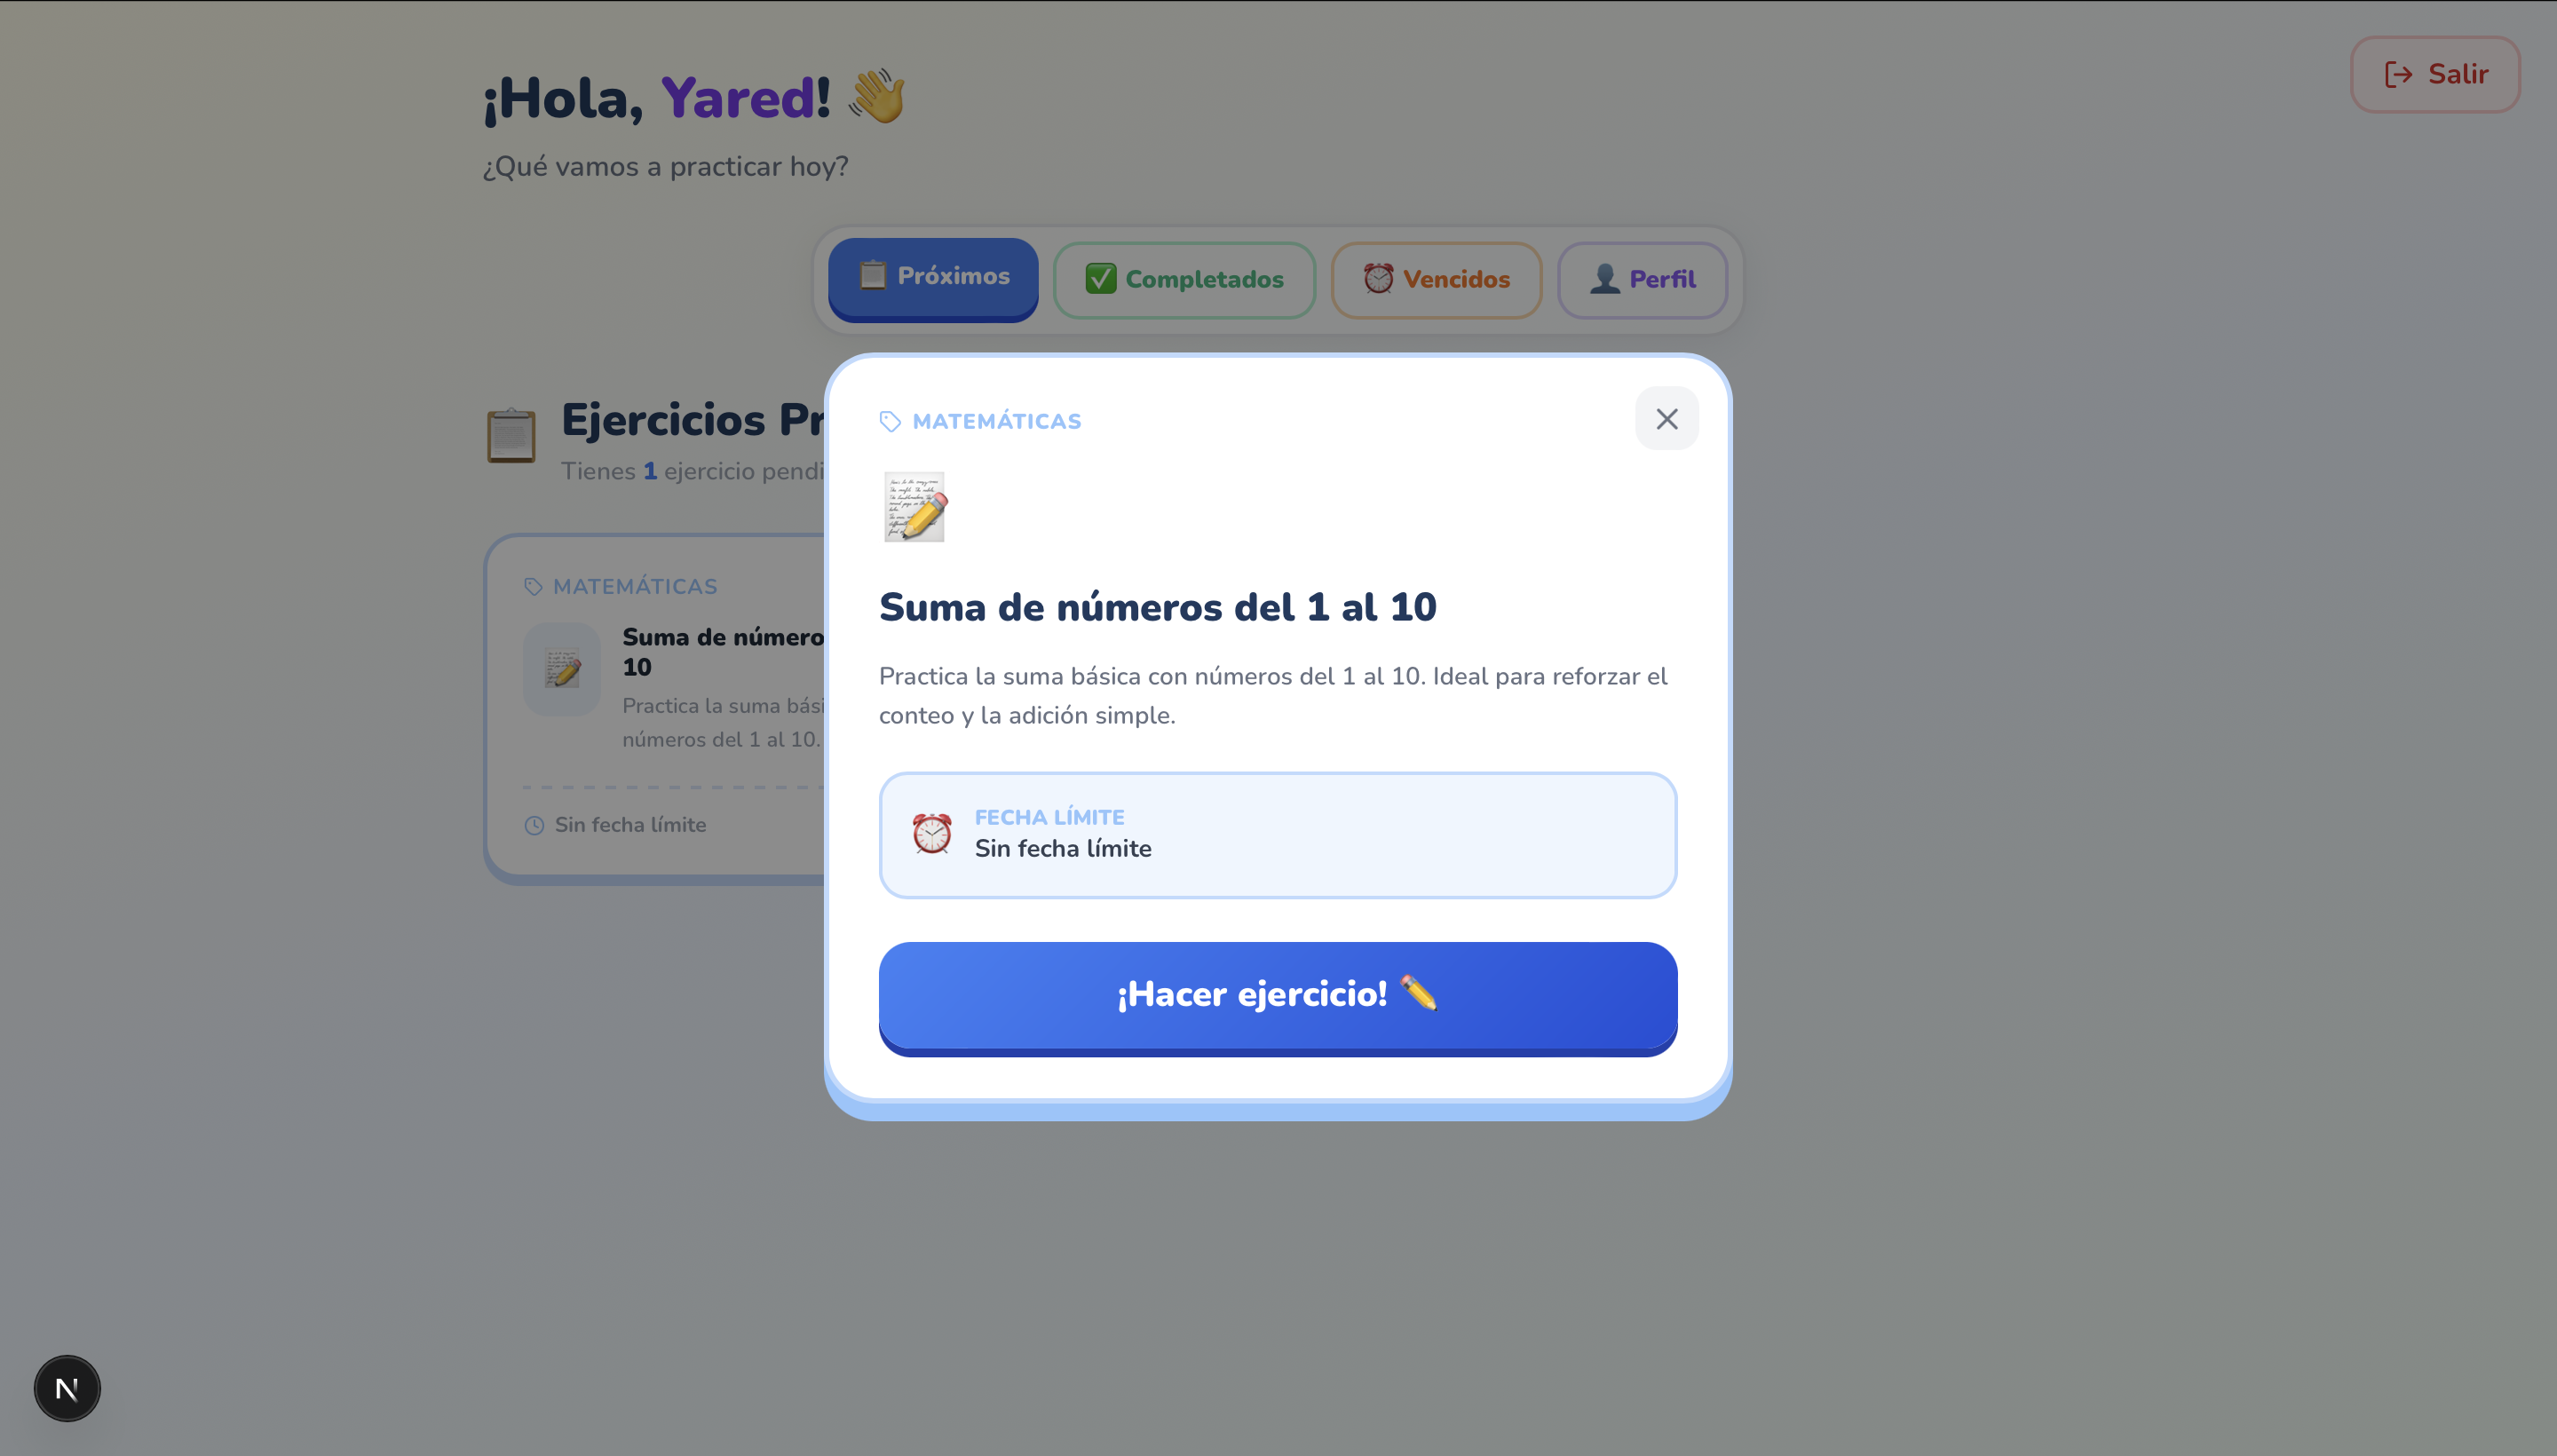
\includegraphics[width=0.7\textwidth]{Imagenes/seleccionEje.png}
    \caption{Visualización de ejercicio a realizar}
    \label{fig:seleccionEje}
\end{figure}

\begin{figure}[H]
    \centering
    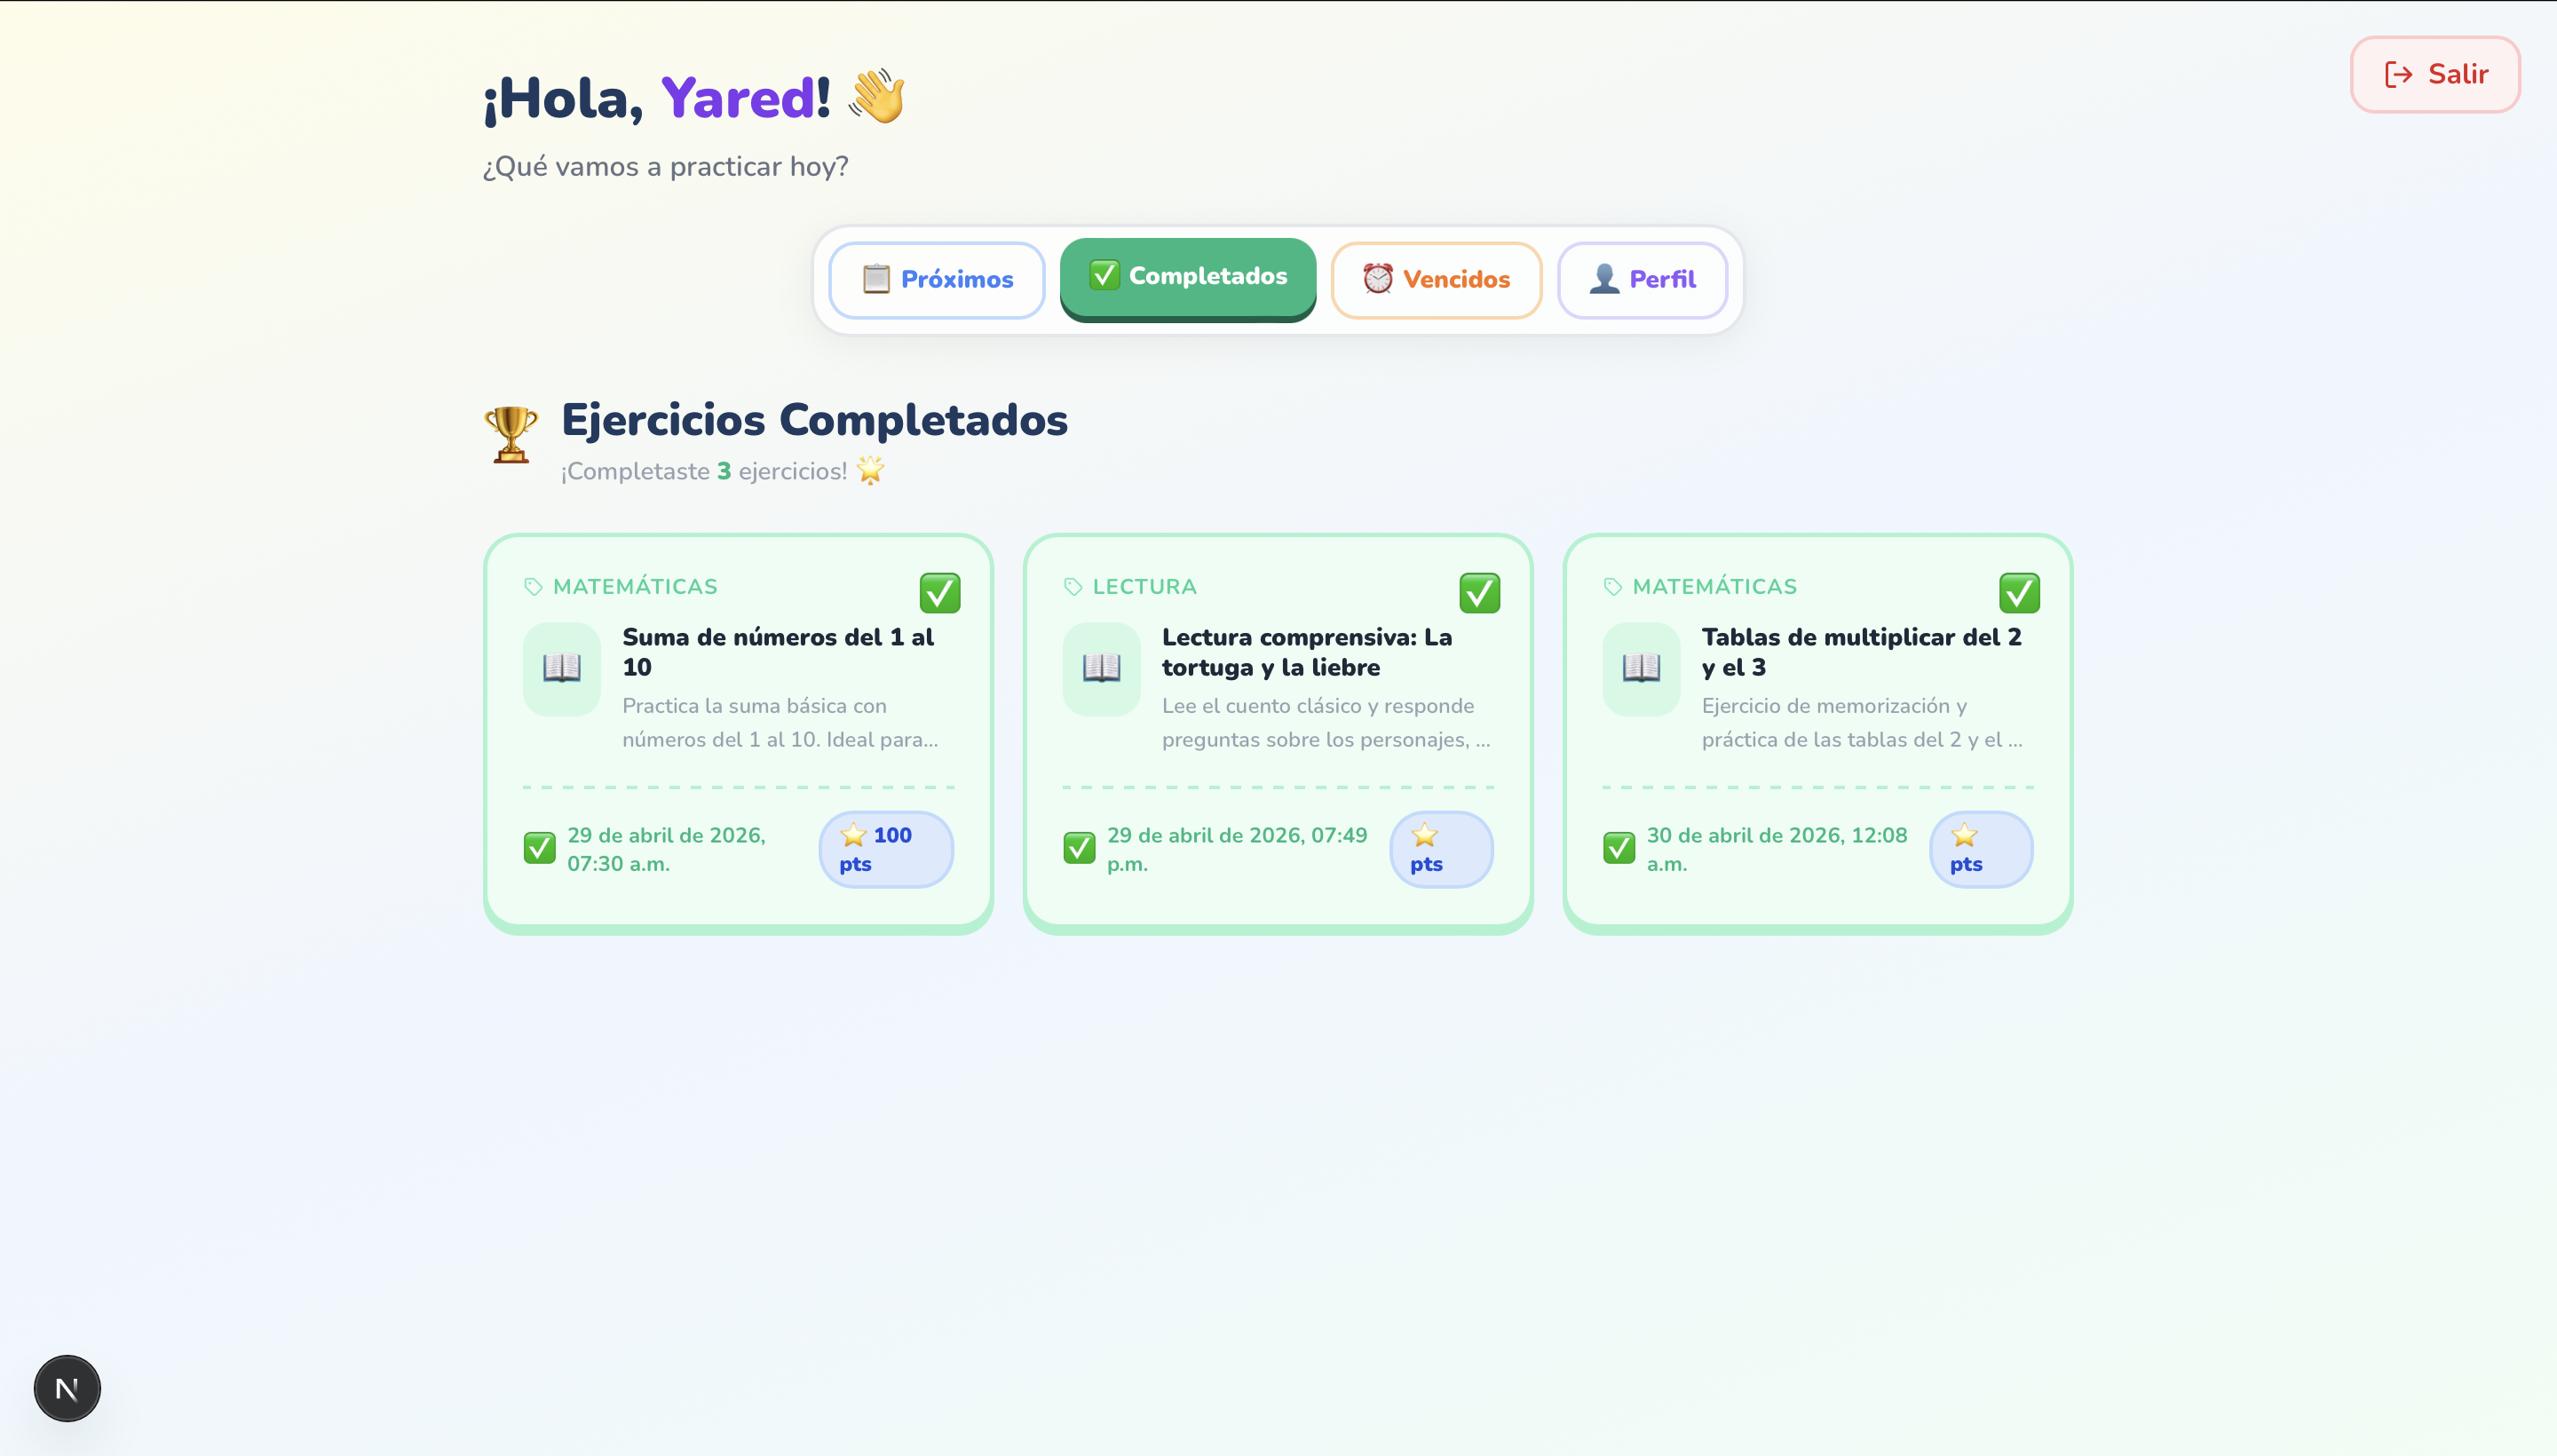
\includegraphics[width=0.7\textwidth]{Imagenes/ejerciciosCompletados.png}
    \caption{Visualización de ejercicios completados por el alumno}
    \label{fig:ejerciciosCompletados}
\end{figure}


\begin{figure}[H]
    \centering
    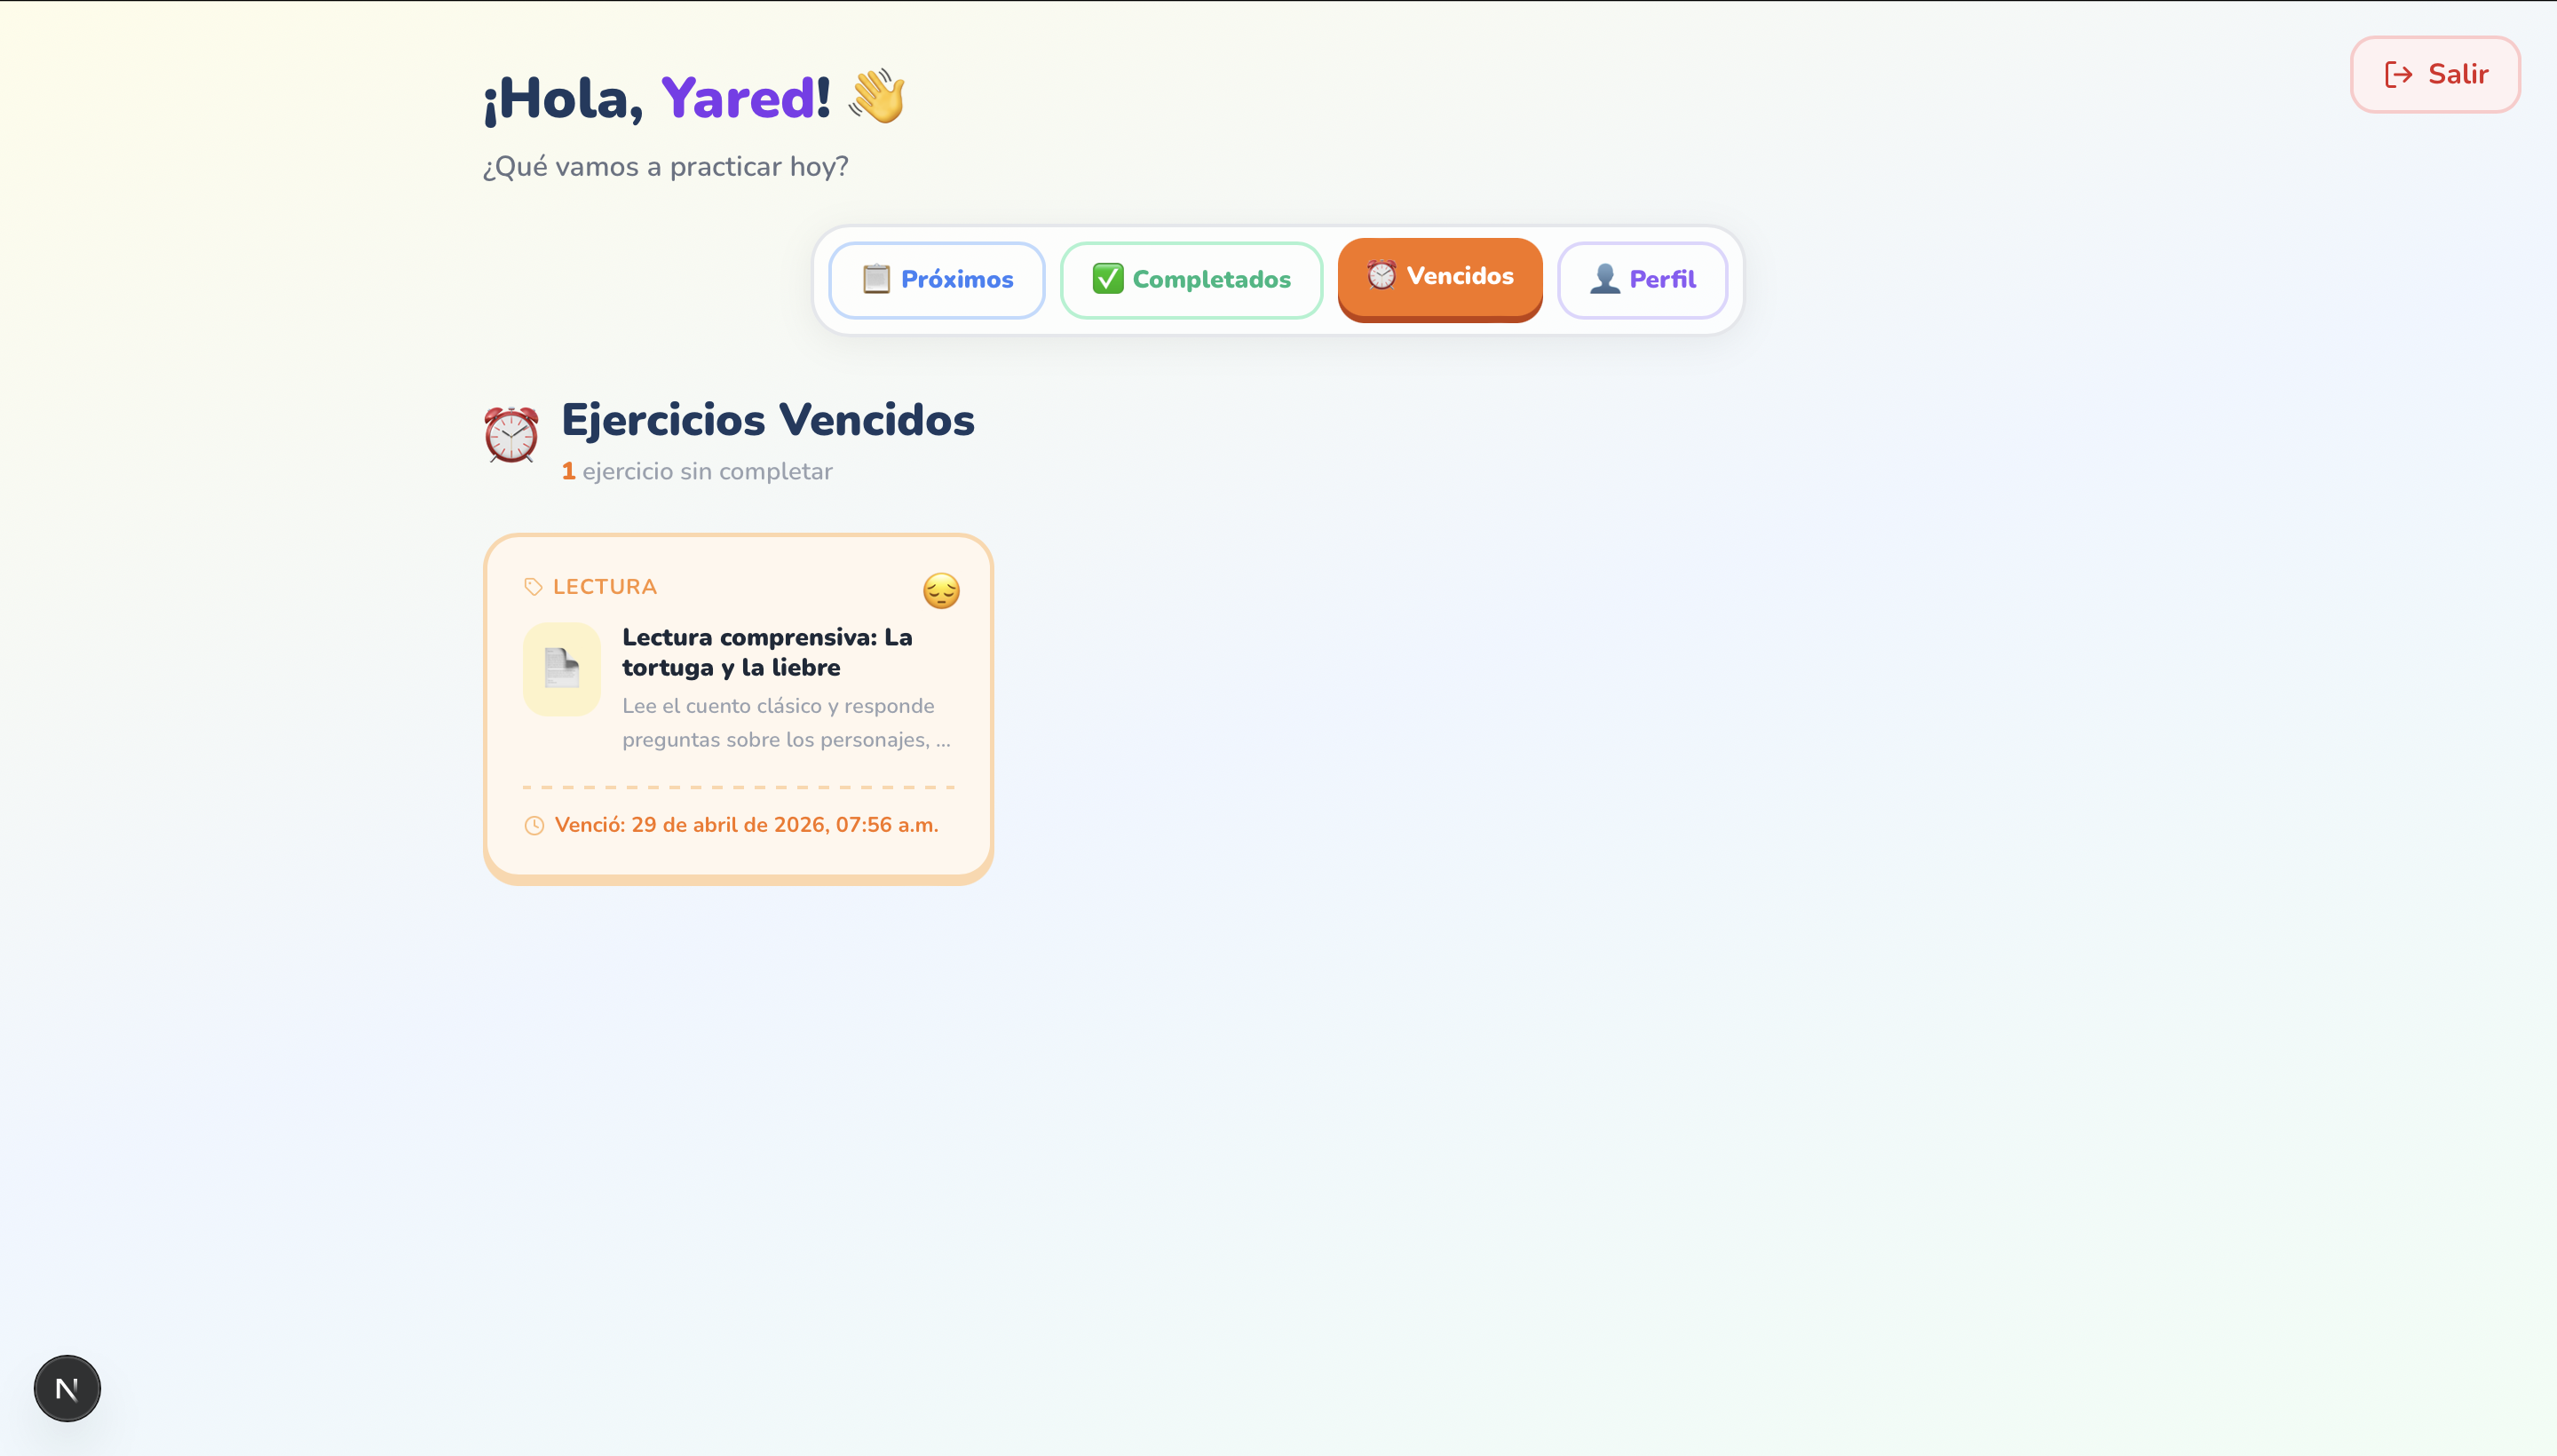
\includegraphics[width=0.7\textwidth]{Imagenes/ejerciciosVencidos.png}
    \caption{Visualización de ejercicios vencidos}
    \label{fig:ejerciciosVencidos}
\end{figure}

\begin{figure}[H]
    \centering
    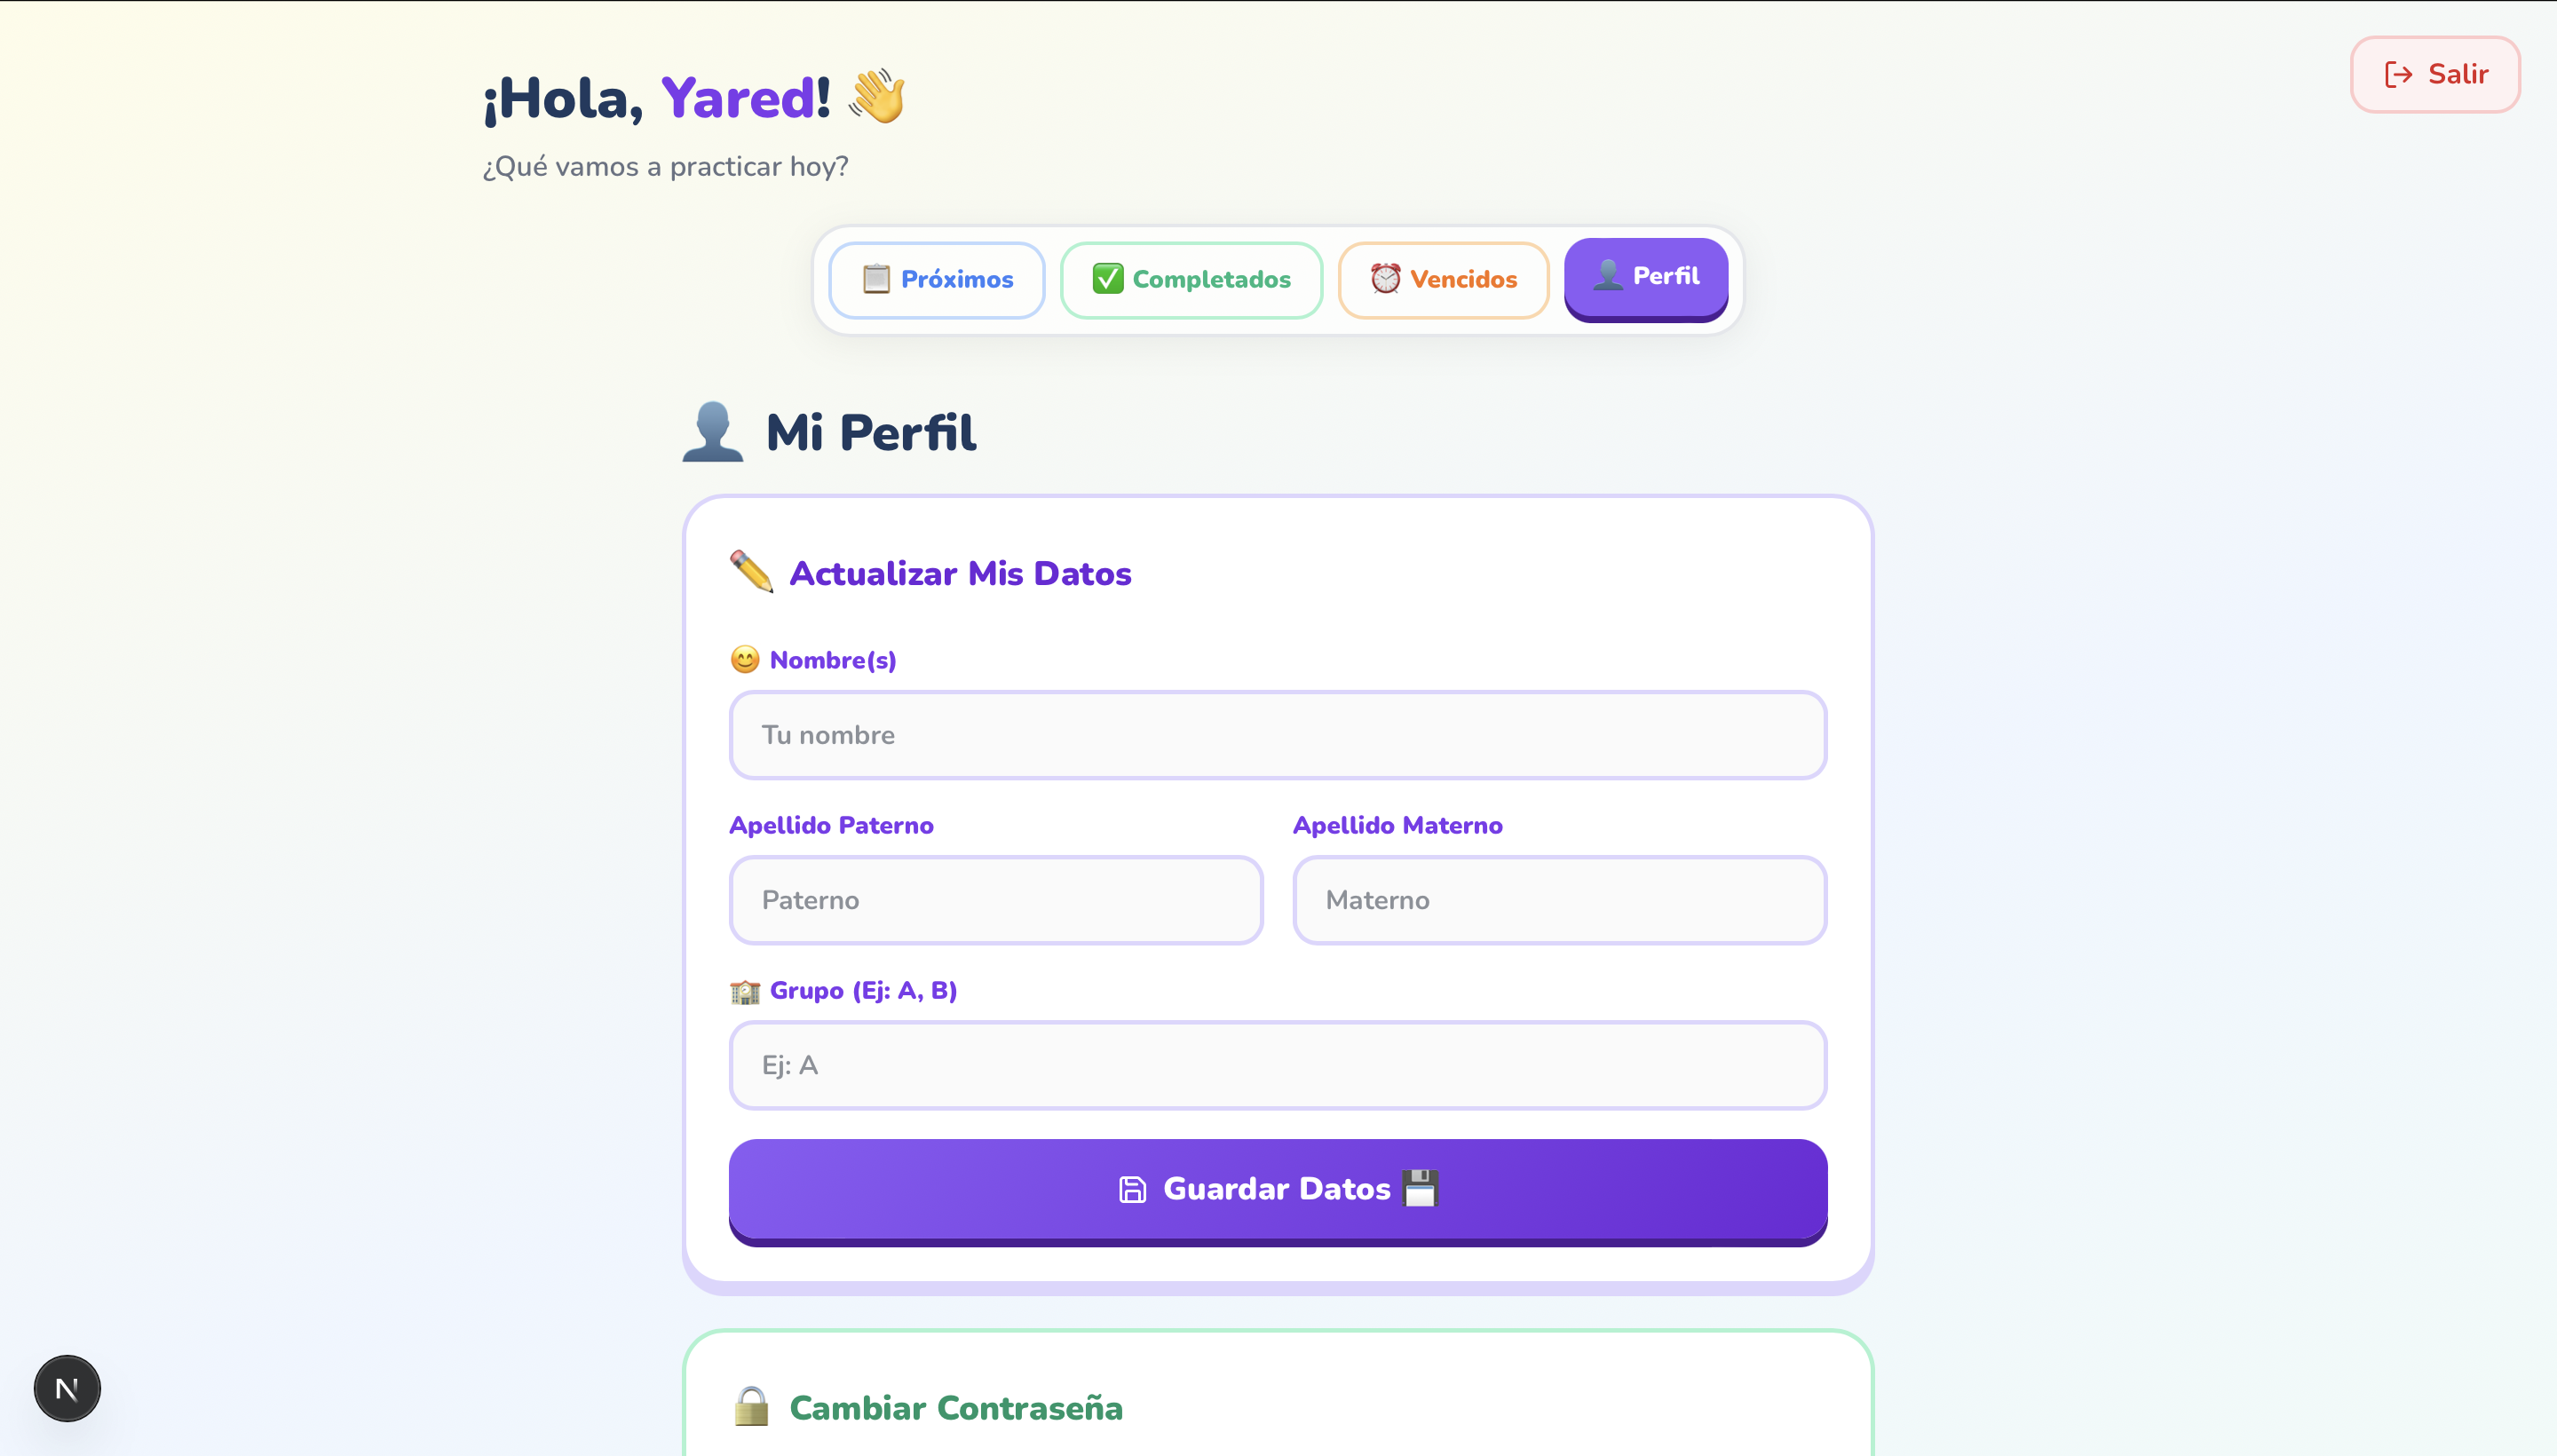
\includegraphics[width=0.7\textwidth]{Imagenes/miperfilA.png}
    \caption{Visualización del perfil del alumno}
    \label{fig:miperfilA}
\end{figure}

\subsubsection{Vista del lienzo digital}

\begin{figure}[H]
    \centering
    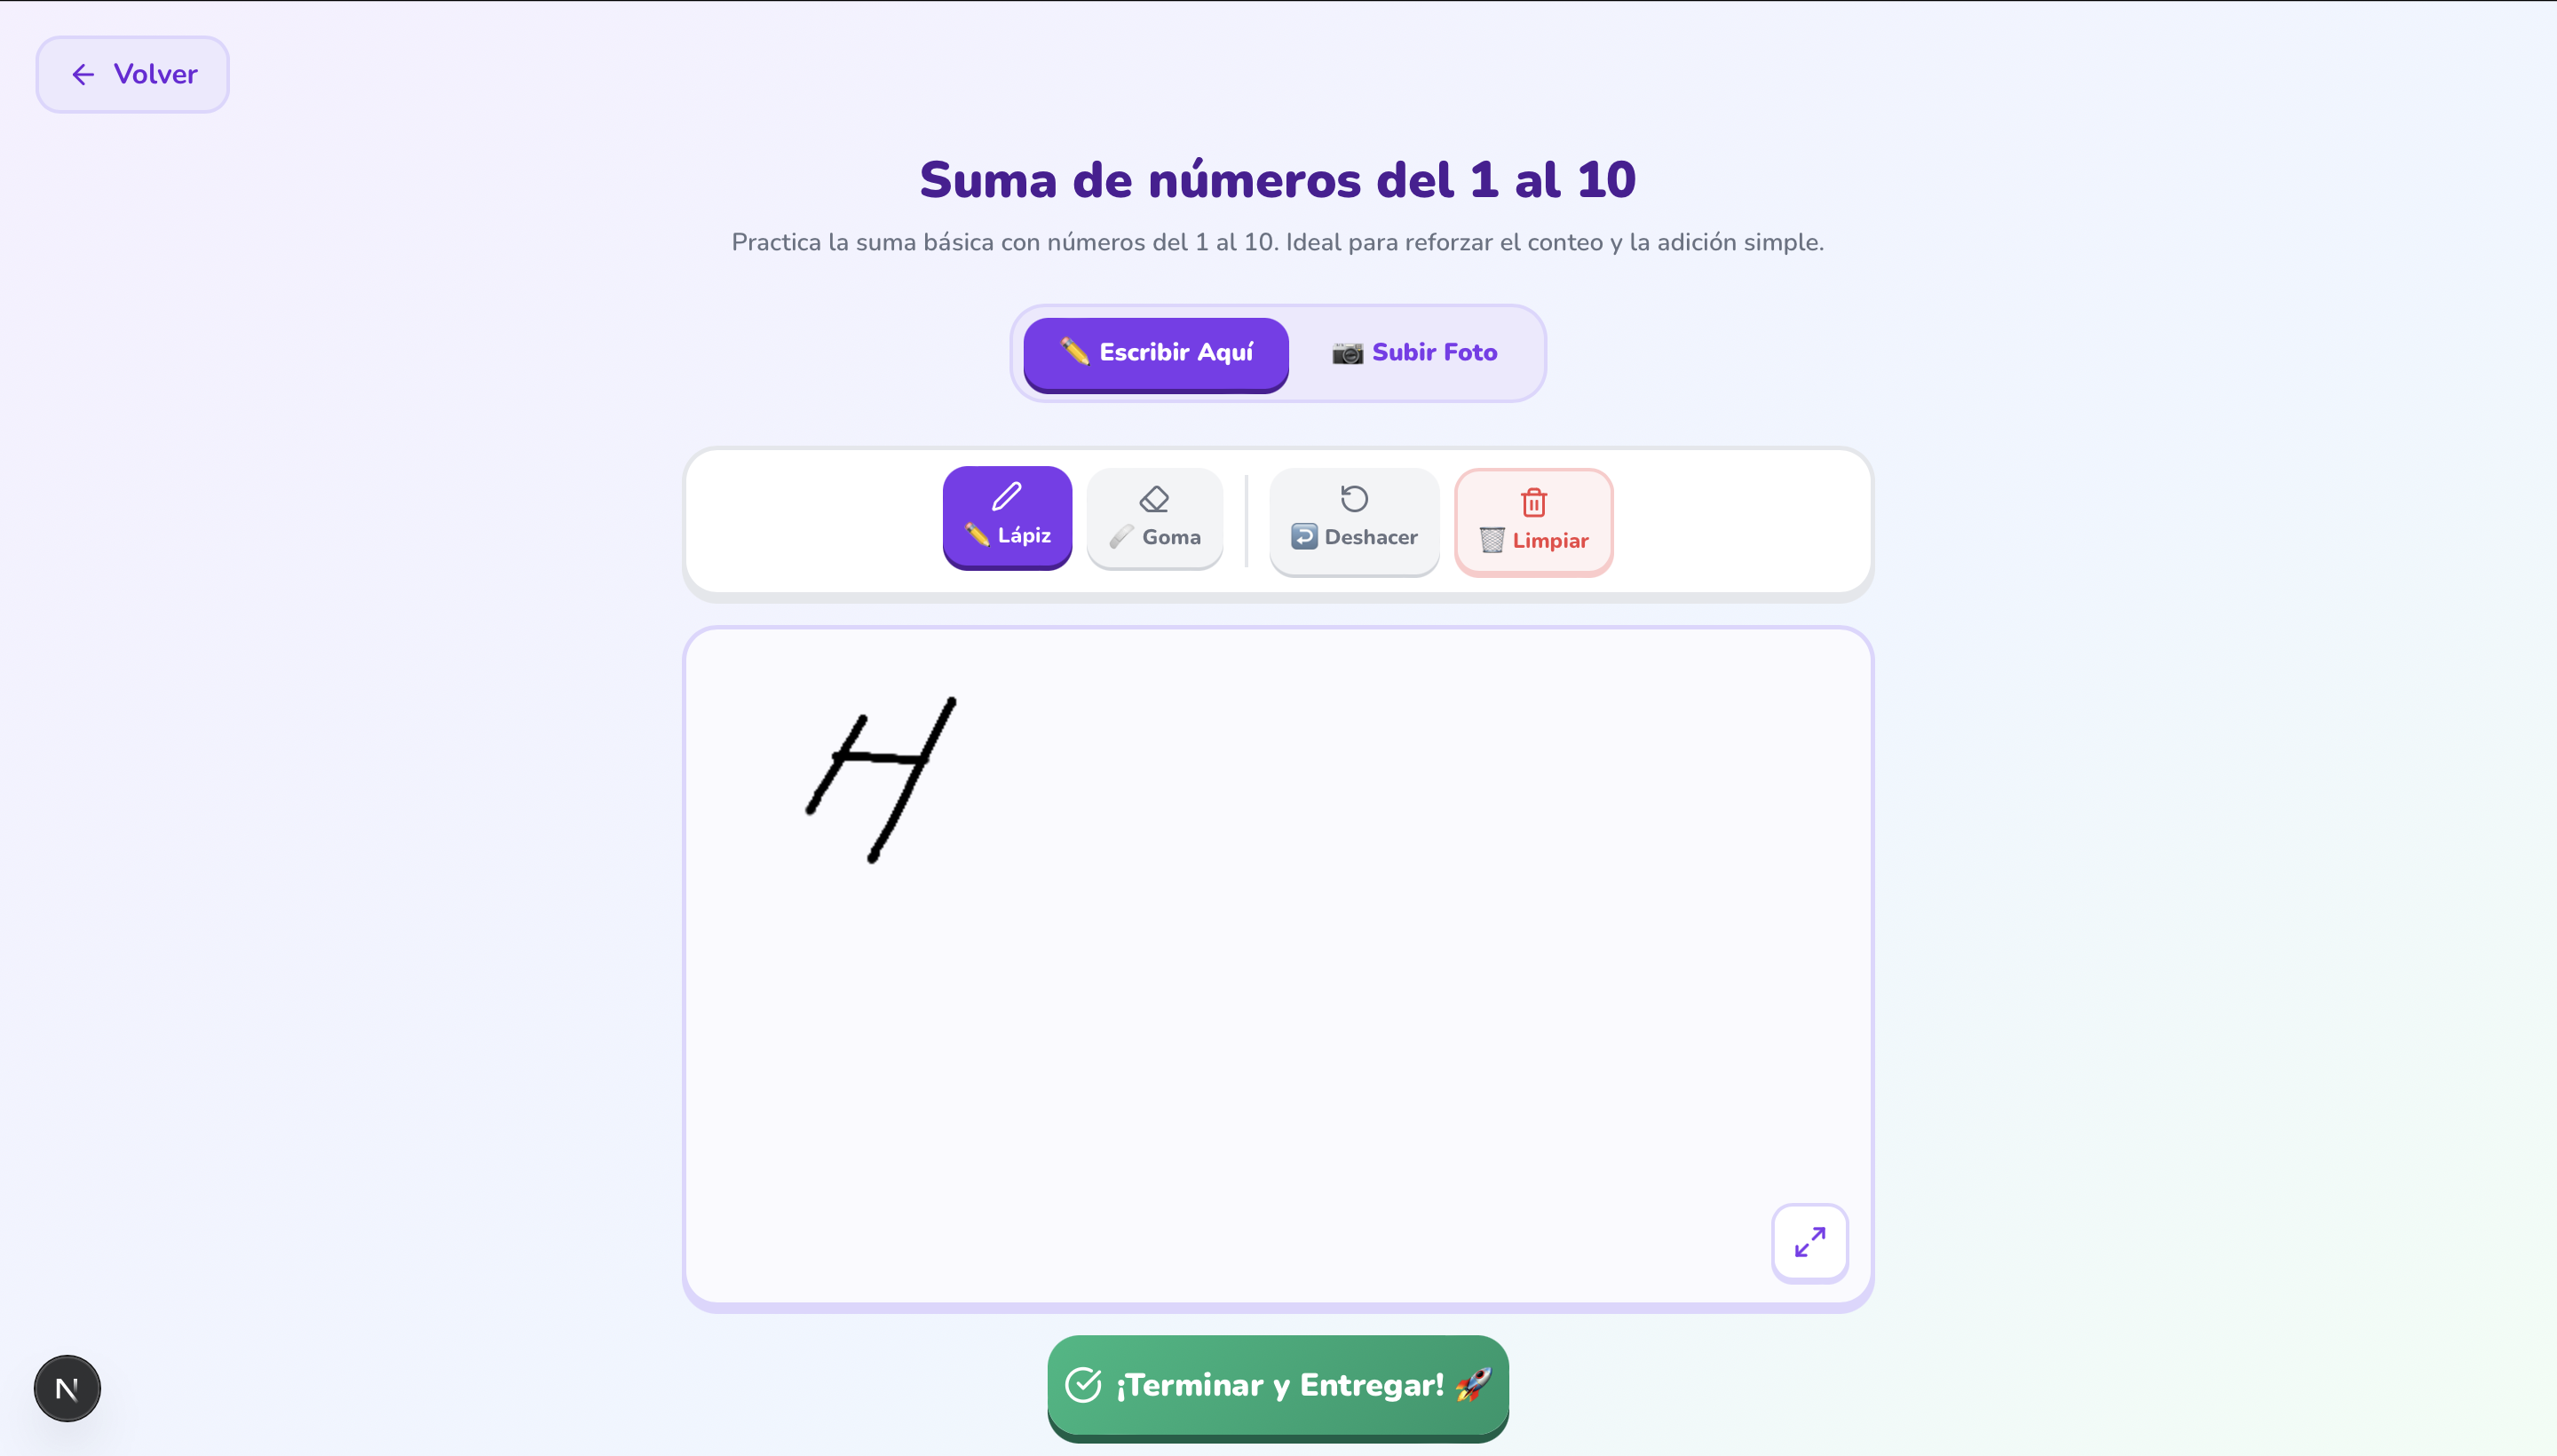
\includegraphics[width=0.7\textwidth]{Imagenes/lienzo.png}
    \caption{Visualización del lienzo digital para realizar ejercicios de escritura}
    \label{fig:lienzo}
\end{figure}


\subsubsection{Vista de captura de escritura}

\begin{figure}[H]
    \centering
    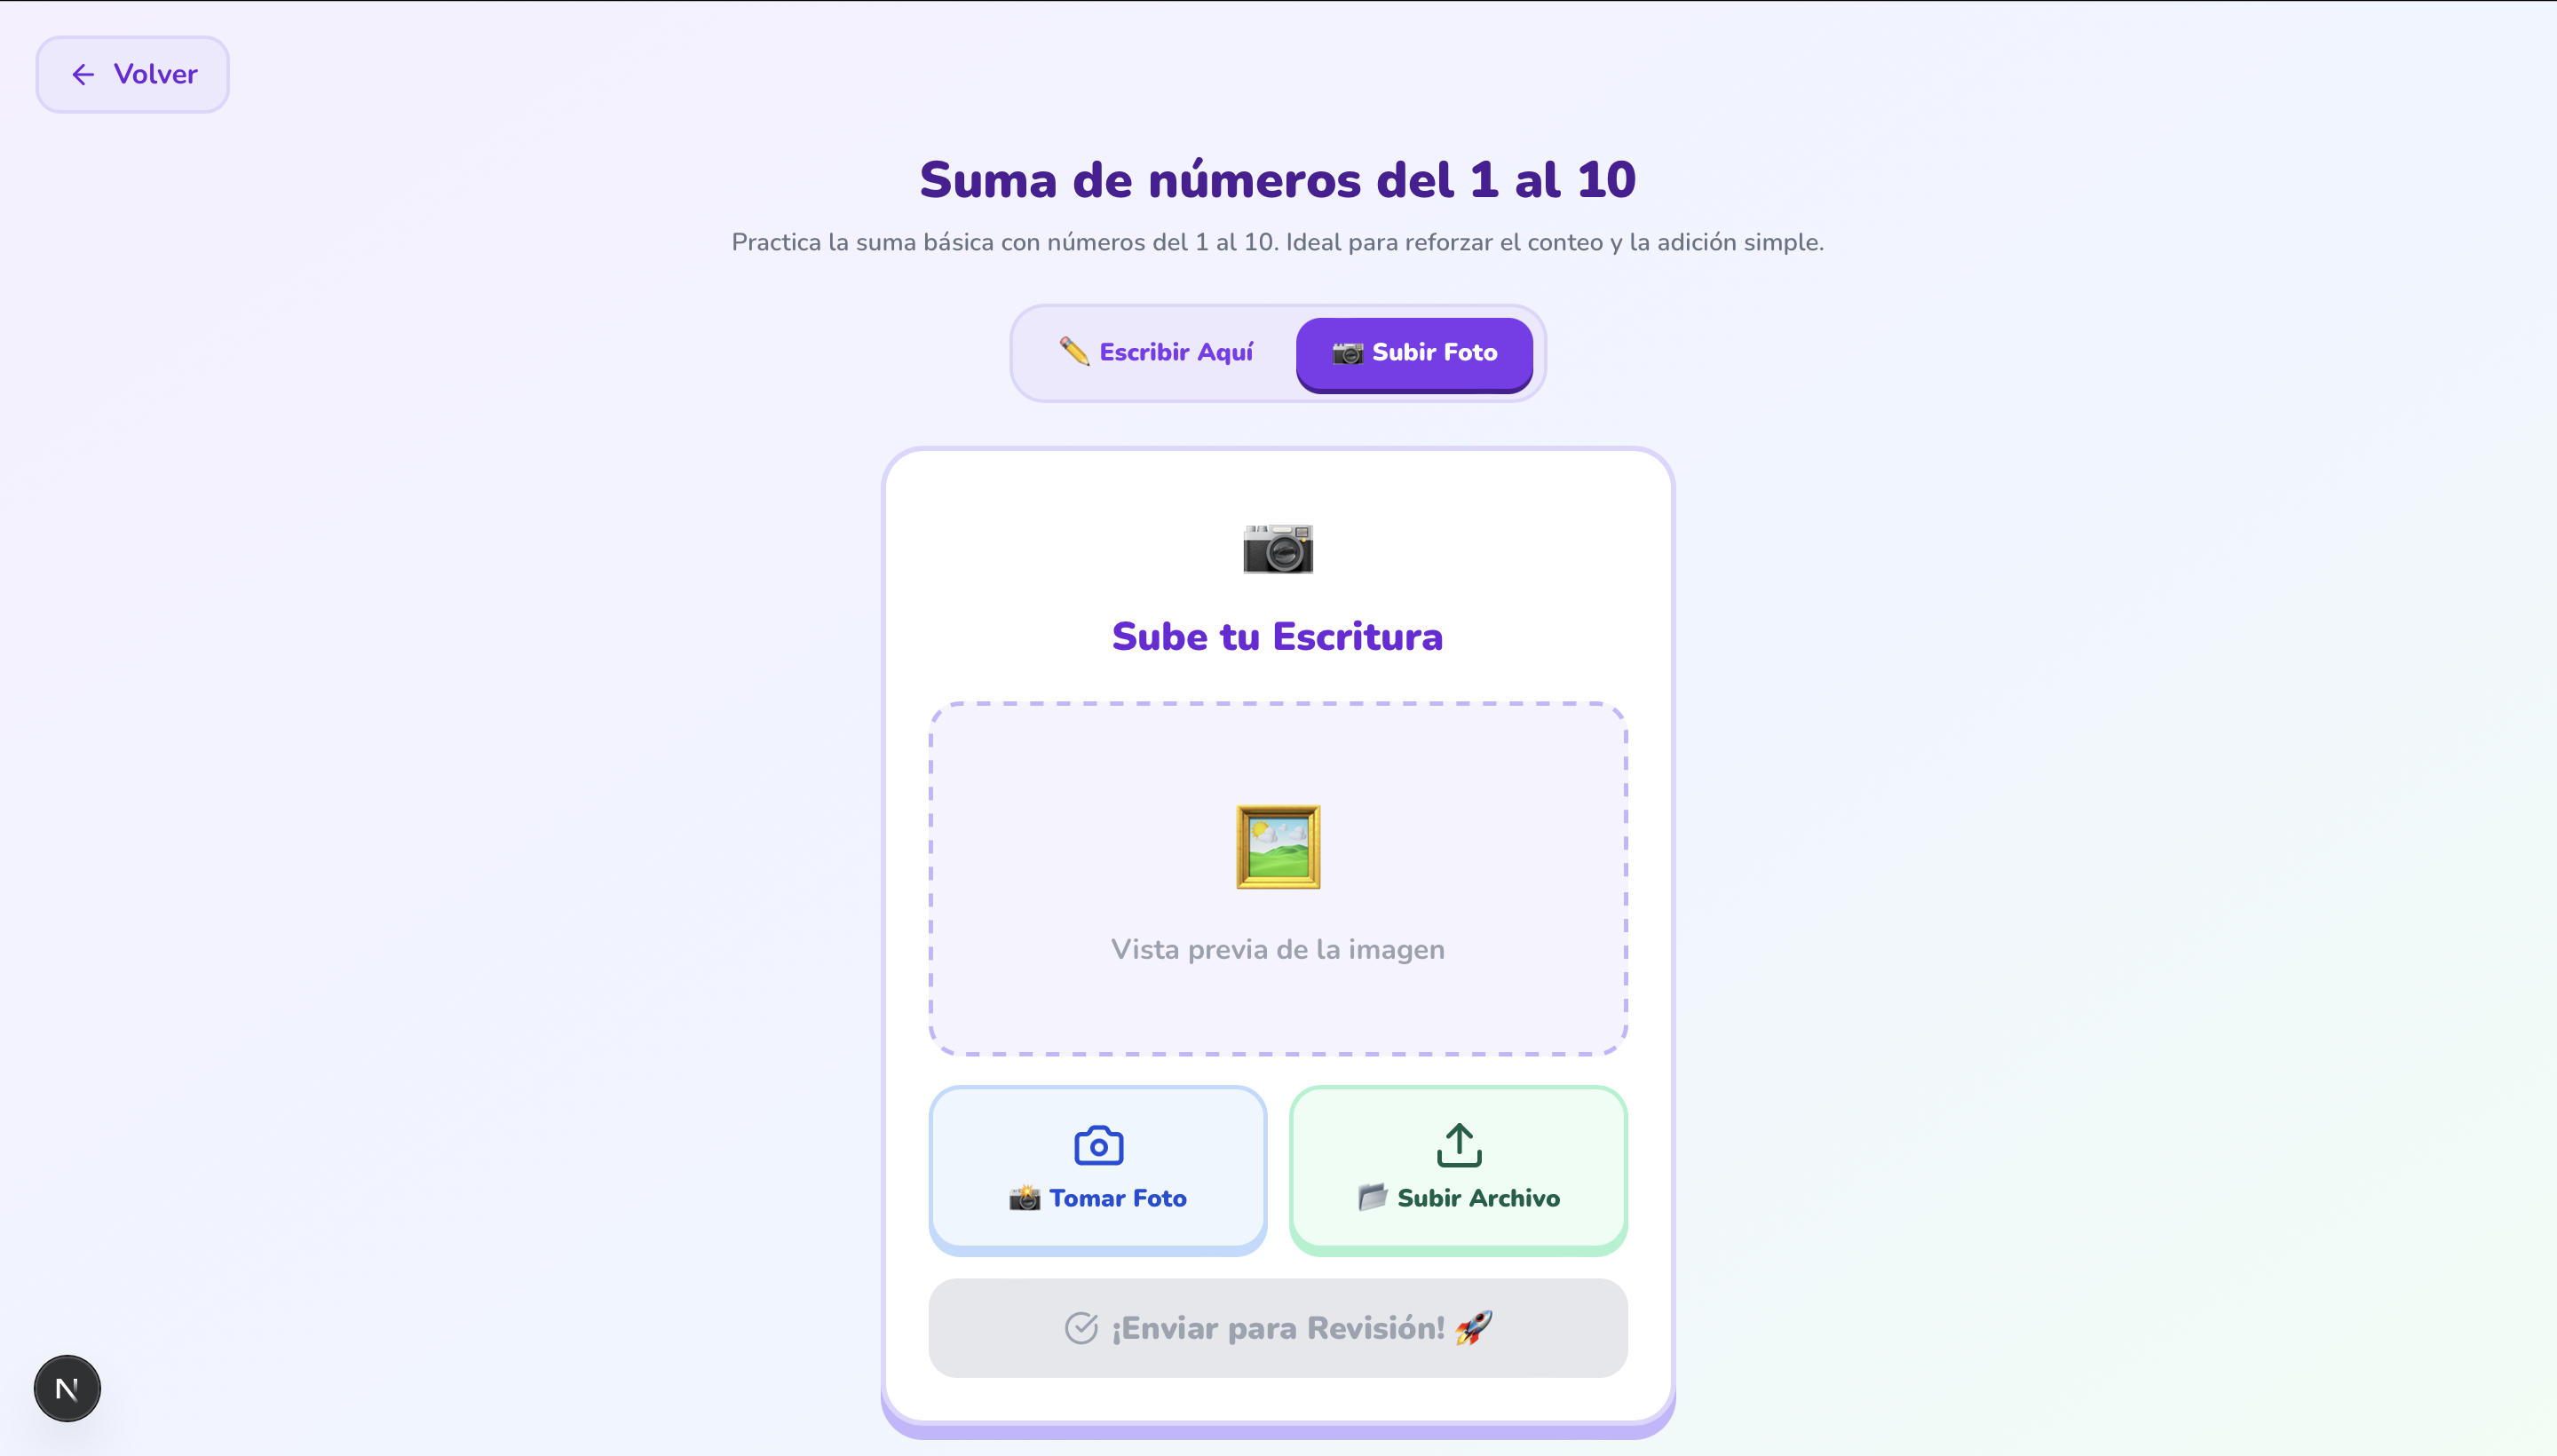
\includegraphics[width=0.7\textwidth]{Imagenes/subirArchivo.png}
    \caption{Visualización de carga de imagen para registrar ejercicios mediante fotografía o archivo}
    \label{fig:subirArchivo}
\end{figure}

\subsubsection{Vista de resultados y retroalimentación}

\begin{figure}[H]
    \centering
    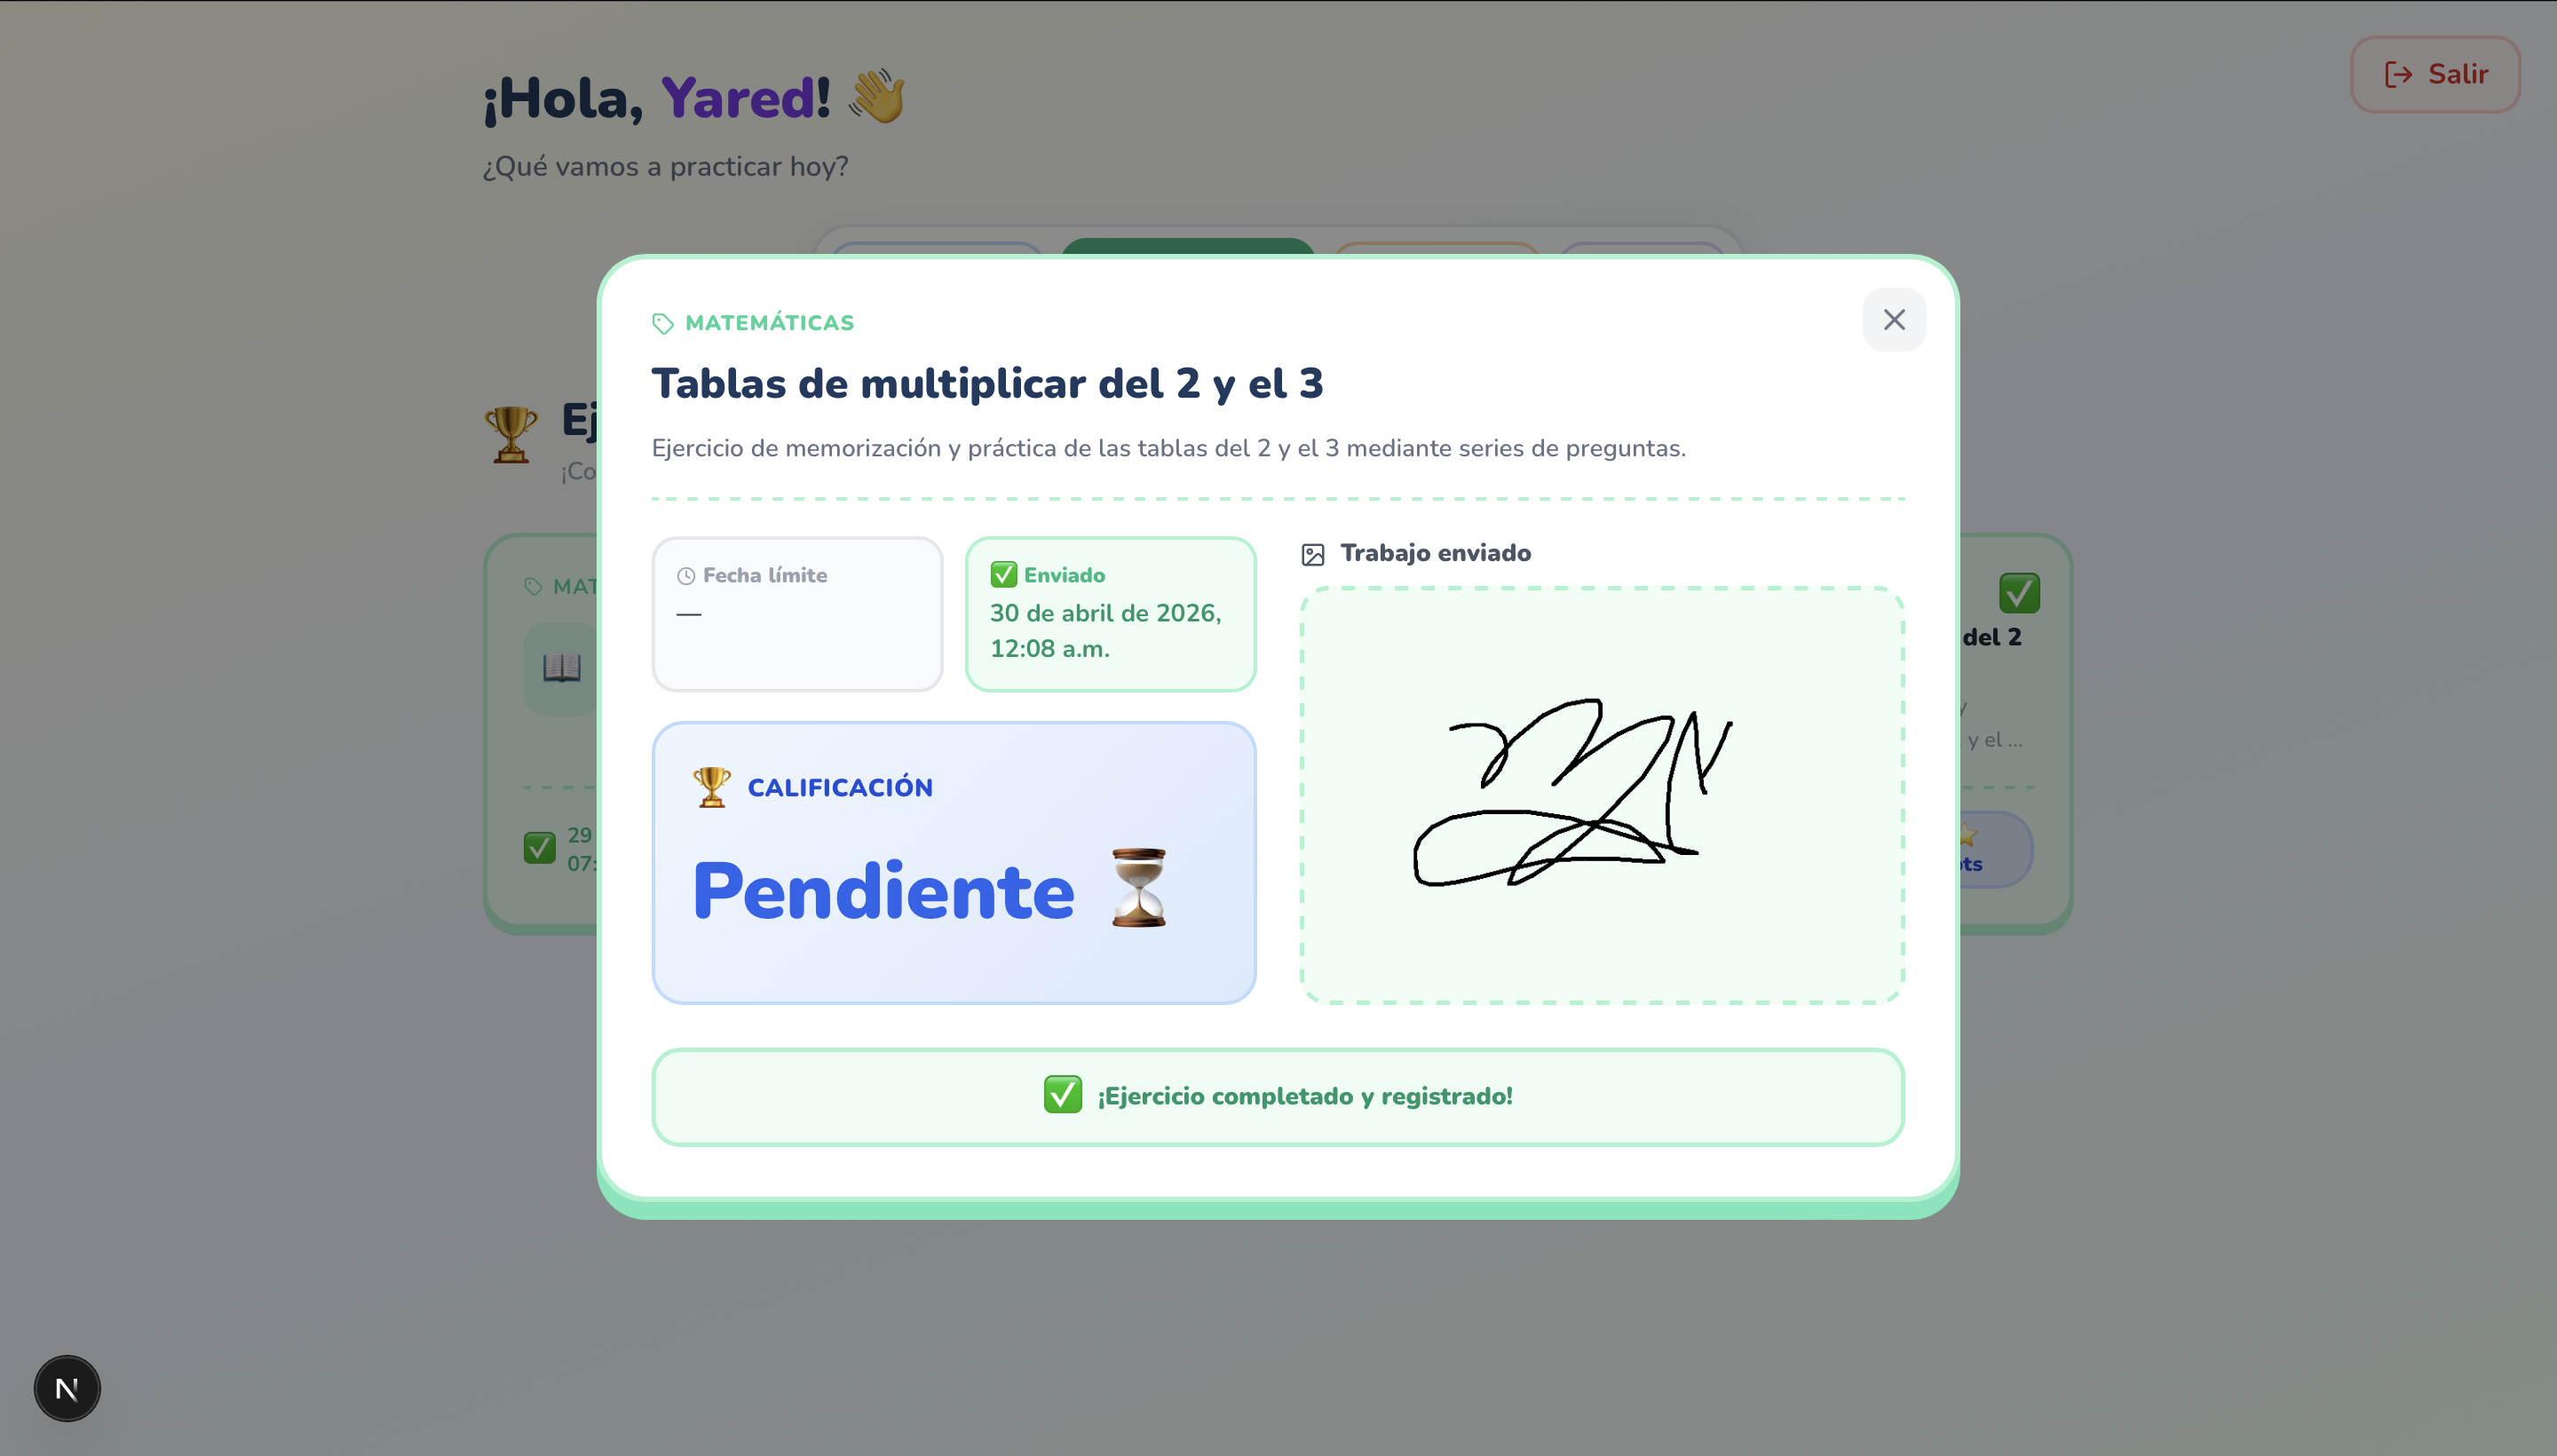
\includegraphics[width=0.7\textwidth]{Imagenes/resultadosEje.png}
    \caption{Visualización de resultados y retroalimentación de ejercicios realizados}
    \label{fig:resultadosEje}
\end{figure}